\chapter{Phase space efficiency}
\label{chap:cpv:phsp}

The definition of the five-dimensional phase space of the \LcTophh\ decays is 
given in \cref{chap:cpv:theory:phsp}.
In this \namecref{chap:cpv:phsp}, the phase space variables in the data will be 
shown, and a description will be given of how a map of the acceptance and 
selection efficiency across those variables is computed.

\section{Distributions in data}
\label{chap:cpv:phsp:data}

\Cref{fig:cpv:phsp:data_1D:pKK,fig:cpv:phsp:data_1D:ppipi} show the 
one-dimensional projections of \msqphm, \msqphp, \msqhh, \thetap, \phip, and 
\phihh\ in the 2012 magnet down datasets, weighted by signal sWeights.
The respective one-dimensional projections from the generator-level \ac{MC}, 
described in \cref{chap:cpv:data:mc:gen}, are overlaid.
\Cref{fig:cpv:phsp:data_2D:pKK,fig:cpv:phsp:data_2D:ppipi} show the 
two-dimensional projections of \msqphp-\msqhh, \msqphm-\msqphp, and 
\msqphp-\msqhh, and illustrate the complex resonant dynamics in the decays.
The child-pair squared mass \msqphp\ is not used as part of the phase space 
parameterisation, but it is shown for completeness.
In all cases, the phase space variables are computed using the momentum vectors 
computed using the \decaytreefitter\ algorithm, where the \phh\ mass is 
constrained to be the nominal \PLambdac\ mass, as described in 
\cref{chap:cpv:data}.

\section{Efficiency modelling}
\label{sec:phsp:eff}

As introduced in \cref{chap:cpv:theory:phsp}, for a meaningful comparison with 
theoretical predictions of \dACP, the measurement must account for any 
sculpting of the \PLambdac\ phase space due to the selection and the \lhcb\ 
acceptance.
This can be done either by providing an efficiency map for theorists to apply 
to their models, or by correcting the measurement with it.
Such a map can be computed by comparing the phase space distributions of the 
signal before and after the selection.
As the signal distributions before the stripping are not available for for 
analysis, the \ac{MC} samples described in \cref{chap:cpv:data:mc} are used.

The phase space efficiency can be considered as a five-dimensional function 
$\eff(\vec{x})$, in the phase space $\vec{x}$, that transforms the original 
distribution $D(\vec{x})$ to the observed one $D'(\vec{x})$
\begin{equation}
  D'(\vec{x}) = \eff(\vec{x})D(\vec{x}).
\end{equation}
If the distributions $D$ and $D'$ were known, the efficiency could be computed 
as the ratio of the two distributions
\begin{equation}
  \eff(\vec{x}) = \frac{D'(\vec{x})}{D(\vec{x})}.
\end{equation}
Taking these distributions from the \ac{MC}, an efficiency \emph{map} could be 
approximated by partitioning the distributions as a five-dimensional histogram 
and taking the ratio between them.
This approach is identical in nature to that defined in the kinematic weighting 
described in \cref{chap:cpv:kinematic_weighting:bdt_method}, as an efficiency 
can be considered as a weighting, and comes with the same drawbacks.
In this particular case, it is hard to reduce the dimensionality of the 
problem, which would make a histogram method more tractable, as it is not clear 
which dimensions would be near-constant in the efficiency, if any.
Indeed, this could be checked by inspecting one-dimensional projections of the 
efficiency, but this neglects correlations between variables which could alter 
the total efficiencies significantly.
To avoid such difficulties, this analysis employs the gradient boosting 
decision tree algorithm, as described in 
\cref{chap:cpv:kinematic_weighting:bdt_method}, in order to estimate the 
efficiency function $\eff(\vec{x})$.

The \ac{BDT} is trained using selected, fully reconstructed truth-matched 
\ac{MC} as the `target', and generator-level \ac{MC} that has not been required 
to be in the \lhcb\ acceptance as the `original' source.
Half the available \ac{MC} is used for training, whilst the other half is used 
for evaluation.
\Cref{fig:cpv:phsp:effs:pKK,fig:cpv:phsp:effs:ppipi} show the one-dimensional 
distributions of the five phase space variables before and after the selection, 
as well as one-dimensional projections of the 5D efficiency function learnt by 
the \ac{BDT}.
For comparison, the ratios between the one-dimensional histograms are also 
shown, with which the function projections show a good agreement.
It can be seen in some cases, such as the \phihh\ projection in both modes, 
that the \ac{BDT} does not capture the visible structure of the histogram 
ratio.
This is likely due to the small sample size used in the training, such that the 
\ac{BDT} does not `see' such structures as statistically significant, modelling 
a comparatively flat efficiency.

To correct the real data for the acceptance and selection efficiencies, they 
are fed through the trained \ac{BDT} and assigned per-decay weights.
These weights are then used in the \chisq\ fit to measure \ARaw.

\begin{figure}
  \centering
  \begin{subfigure}{0.4\textwidth}
    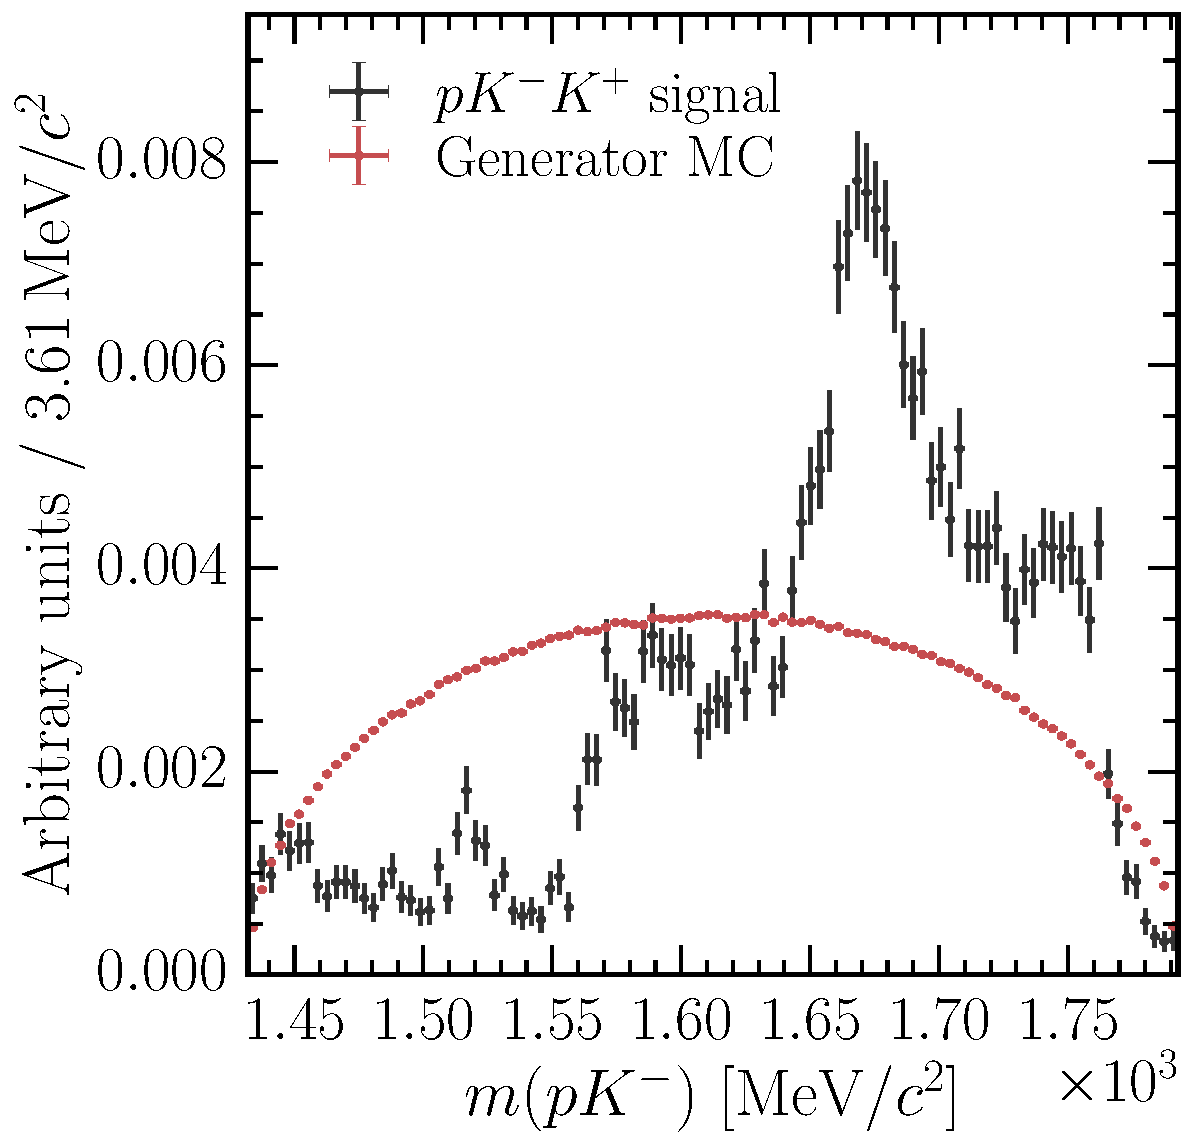
\includegraphics[width=\textwidth]{cpv/phase_space/LcTopKK_2012_MagDown_Lc_p_h1_M}
    \label{fig:cpv:phsp:data:pKK:msqphm}
  \end{subfigure}
  \begin{subfigure}{0.4\textwidth}
    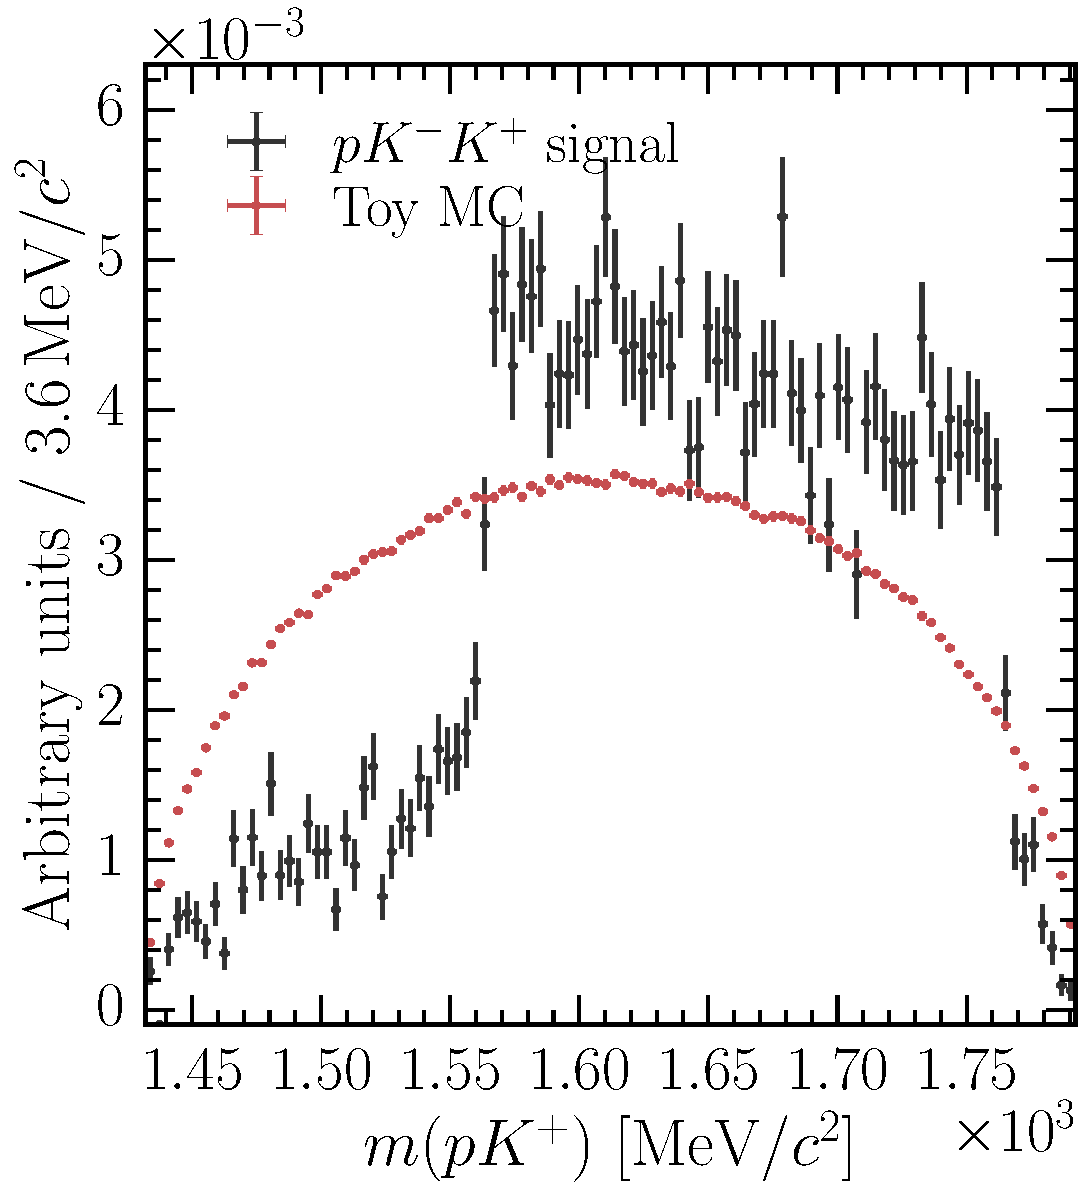
\includegraphics[width=\textwidth]{cpv/phase_space/LcTopKK_2012_MagDown_Lc_p_h2_M}
    \label{fig:cpv:phsp:data:pKK:msqphp}
  \end{subfigure}
  \begin{subfigure}{0.4\textwidth}
    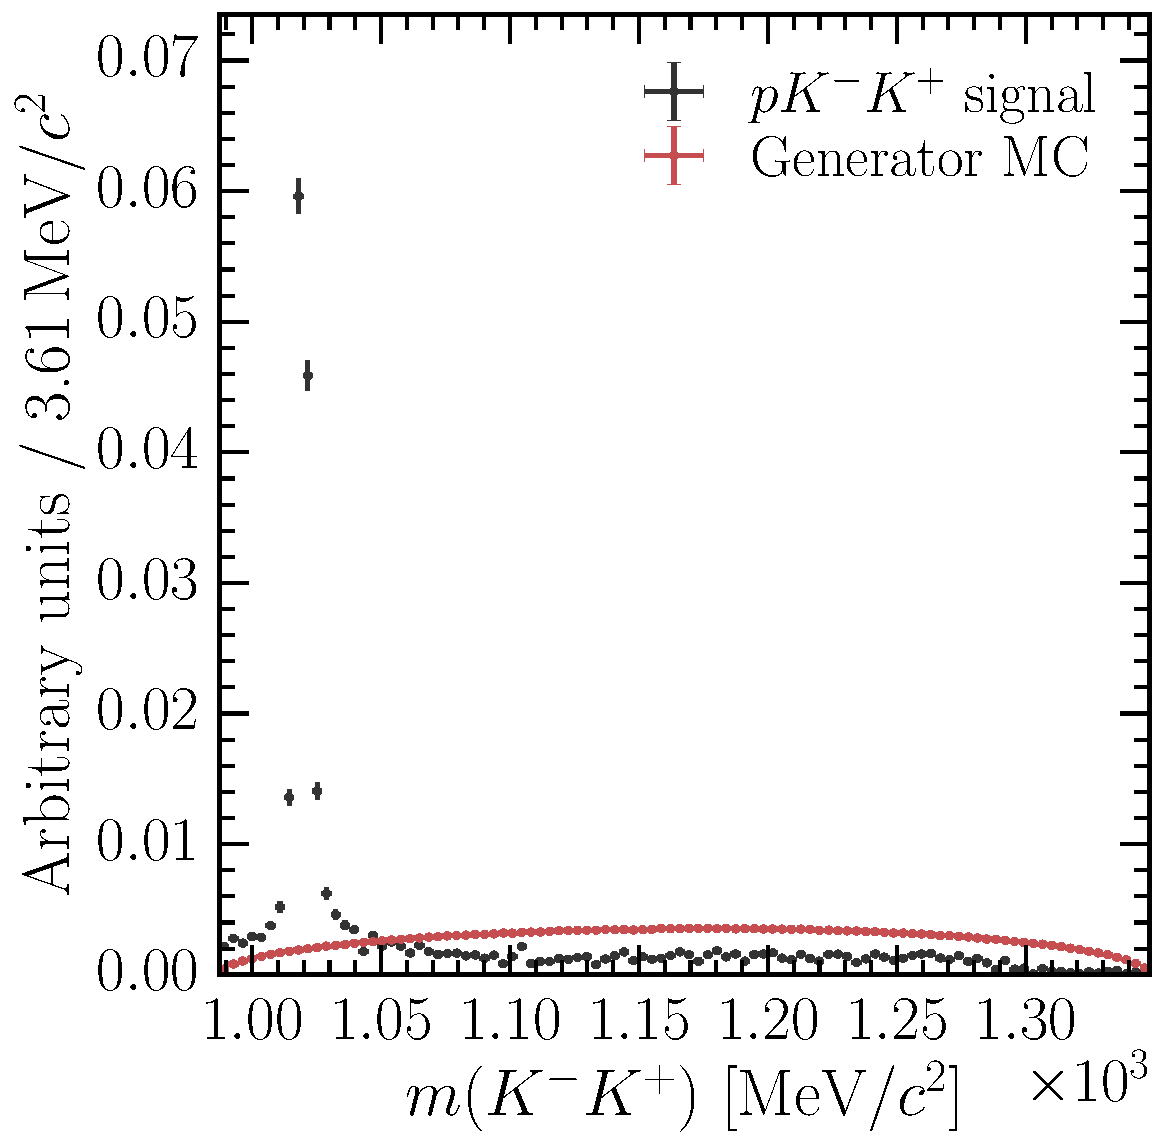
\includegraphics[width=\textwidth]{cpv/phase_space/LcTopKK_2012_MagDown_Lc_h1_h2_M}
    \label{fig:cpv:phsp:data:pKK:msqhh}
  \end{subfigure}
  \begin{subfigure}{0.4\textwidth}
    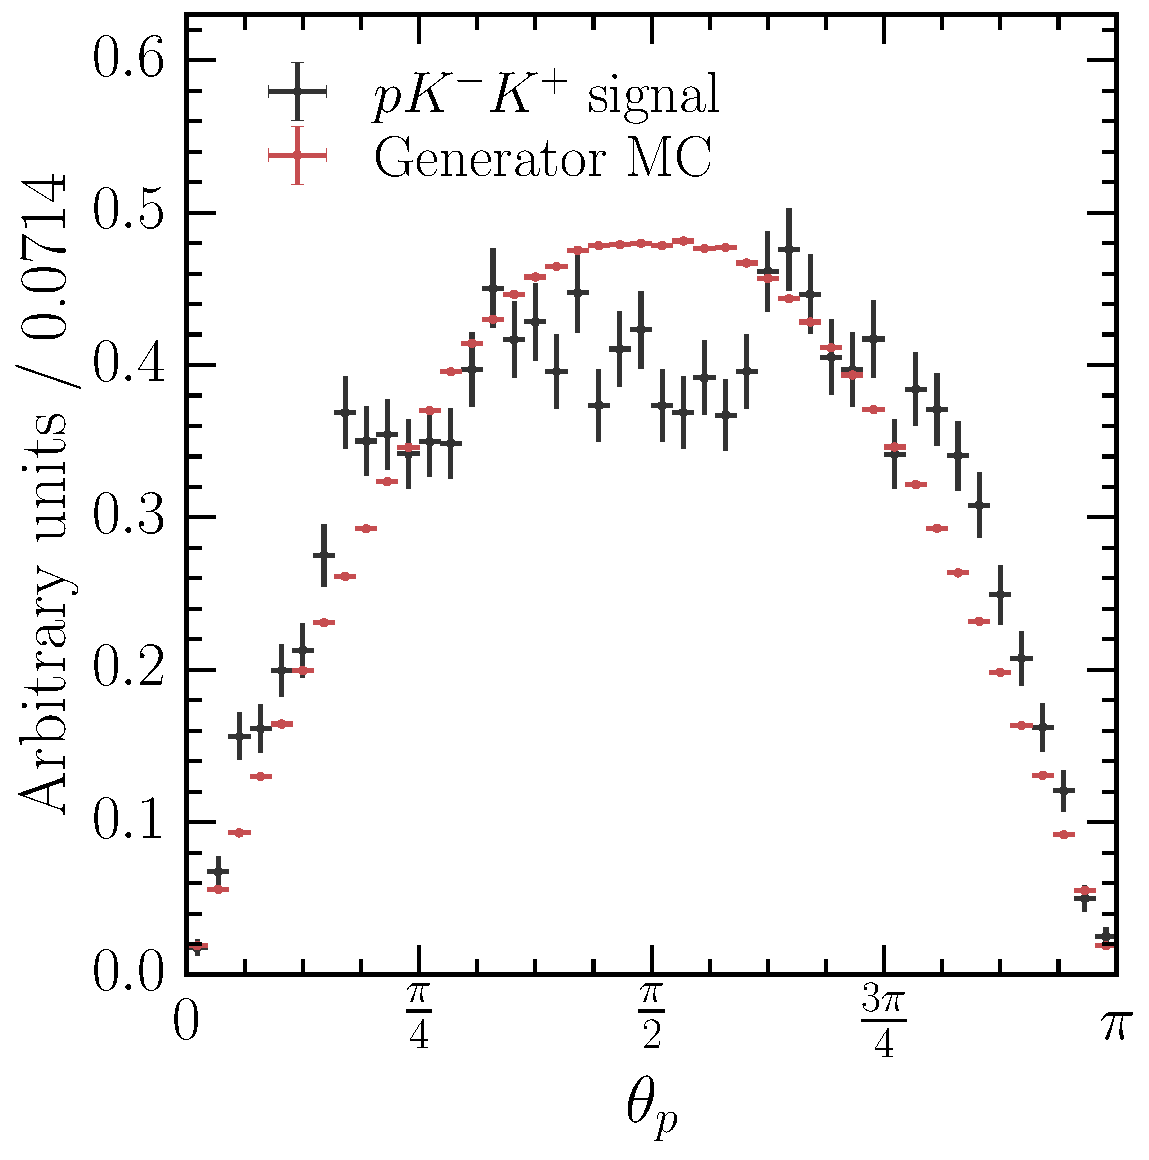
\includegraphics[width=\textwidth]{cpv/phase_space/LcTopKK_2012_MagDown_Lc_phsp_p_theta}
    \label{fig:cpv:phsp:data:pKK:proton_theta}
  \end{subfigure}
  \begin{subfigure}{0.4\textwidth}
    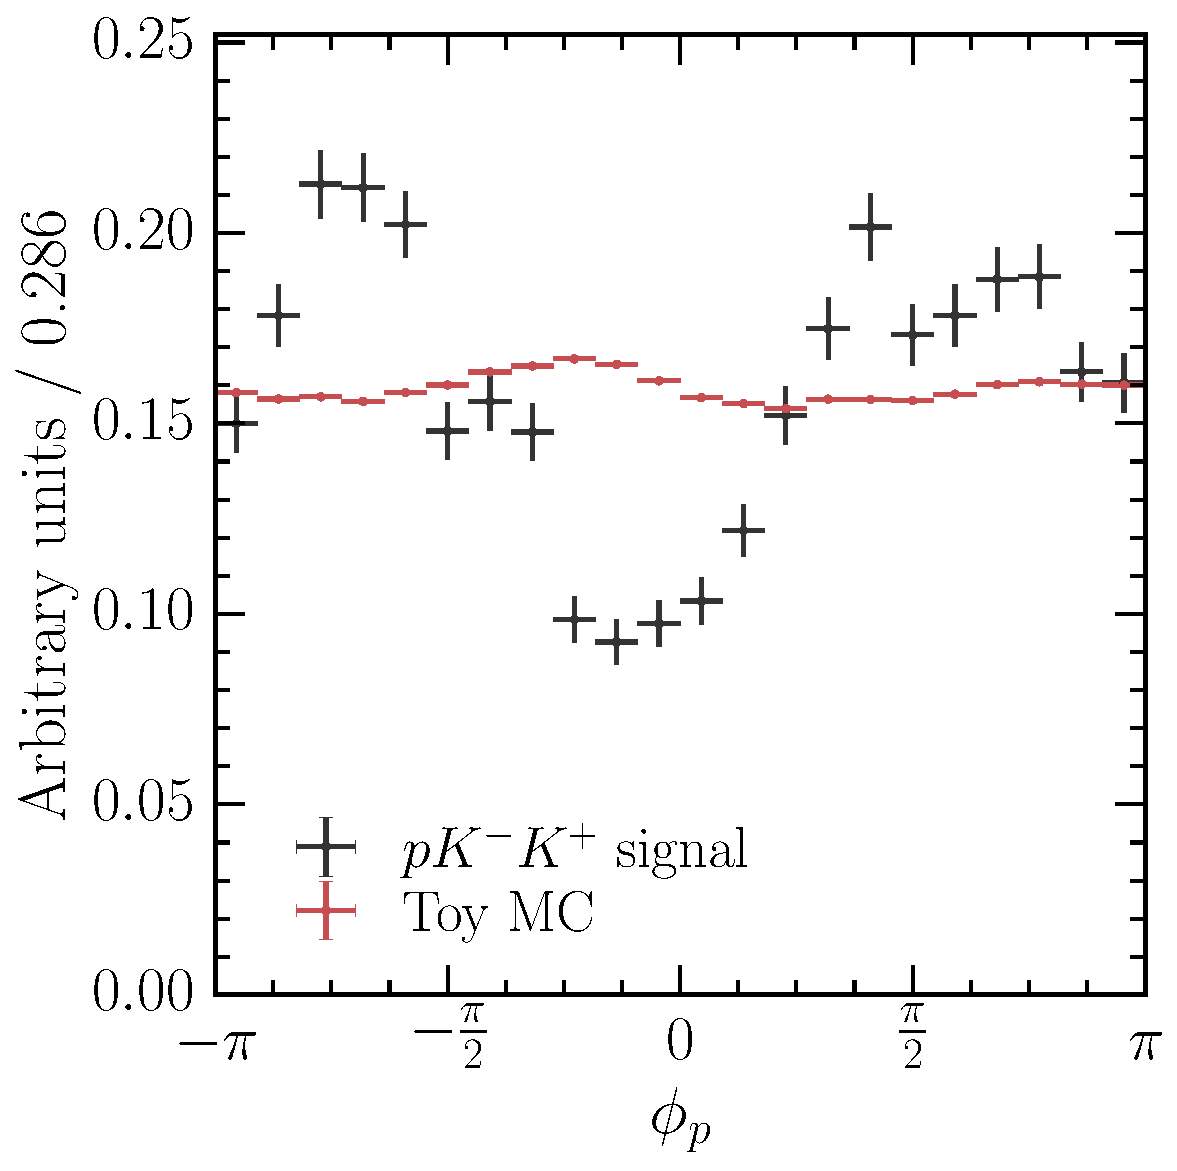
\includegraphics[width=\textwidth]{cpv/phase_space/LcTopKK_2012_MagDown_Lc_phsp_p_phi}
    \label{fig:cpv:phsp:data:pKK:proton_phi}
  \end{subfigure}
  \begin{subfigure}{0.4\textwidth}
    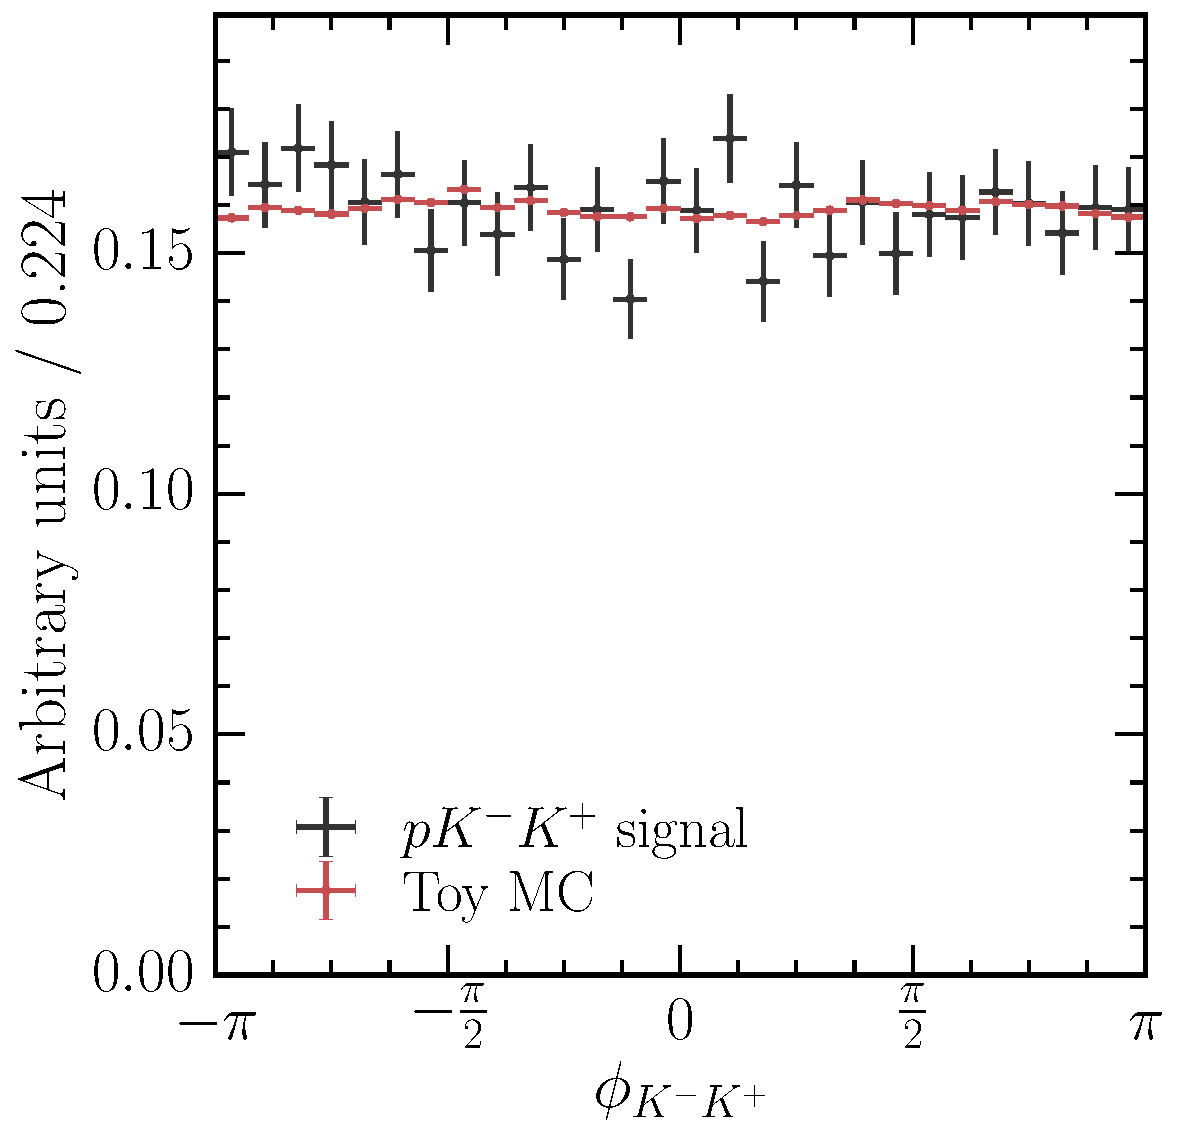
\includegraphics[width=\textwidth]{cpv/phase_space/LcTopKK_2012_MagDown_Lc_phsp_h1_h2_phi}
    \label{fig:cpv:phsp:data:pKK:h1_h2_phi}
  \end{subfigure}
  \caption{%
    % TODO update these plots to those using the LHCb generator-level MC
    One dimensional projections of the \LcTopKK\ phase space in the fully 
    selected 2012 magnet down data, weighted by signal sWeights, along with the 
    respective one-dimensional projections from the generator-level \ac{MC}, 
    described in \cref{chap:cpv:data:mc:gen}.
  }
  \label{fig:cpv:phsp:data_1D:pKK}
\end{figure}

\begin{figure}
  \begin{subfigure}{0.5\textwidth}
    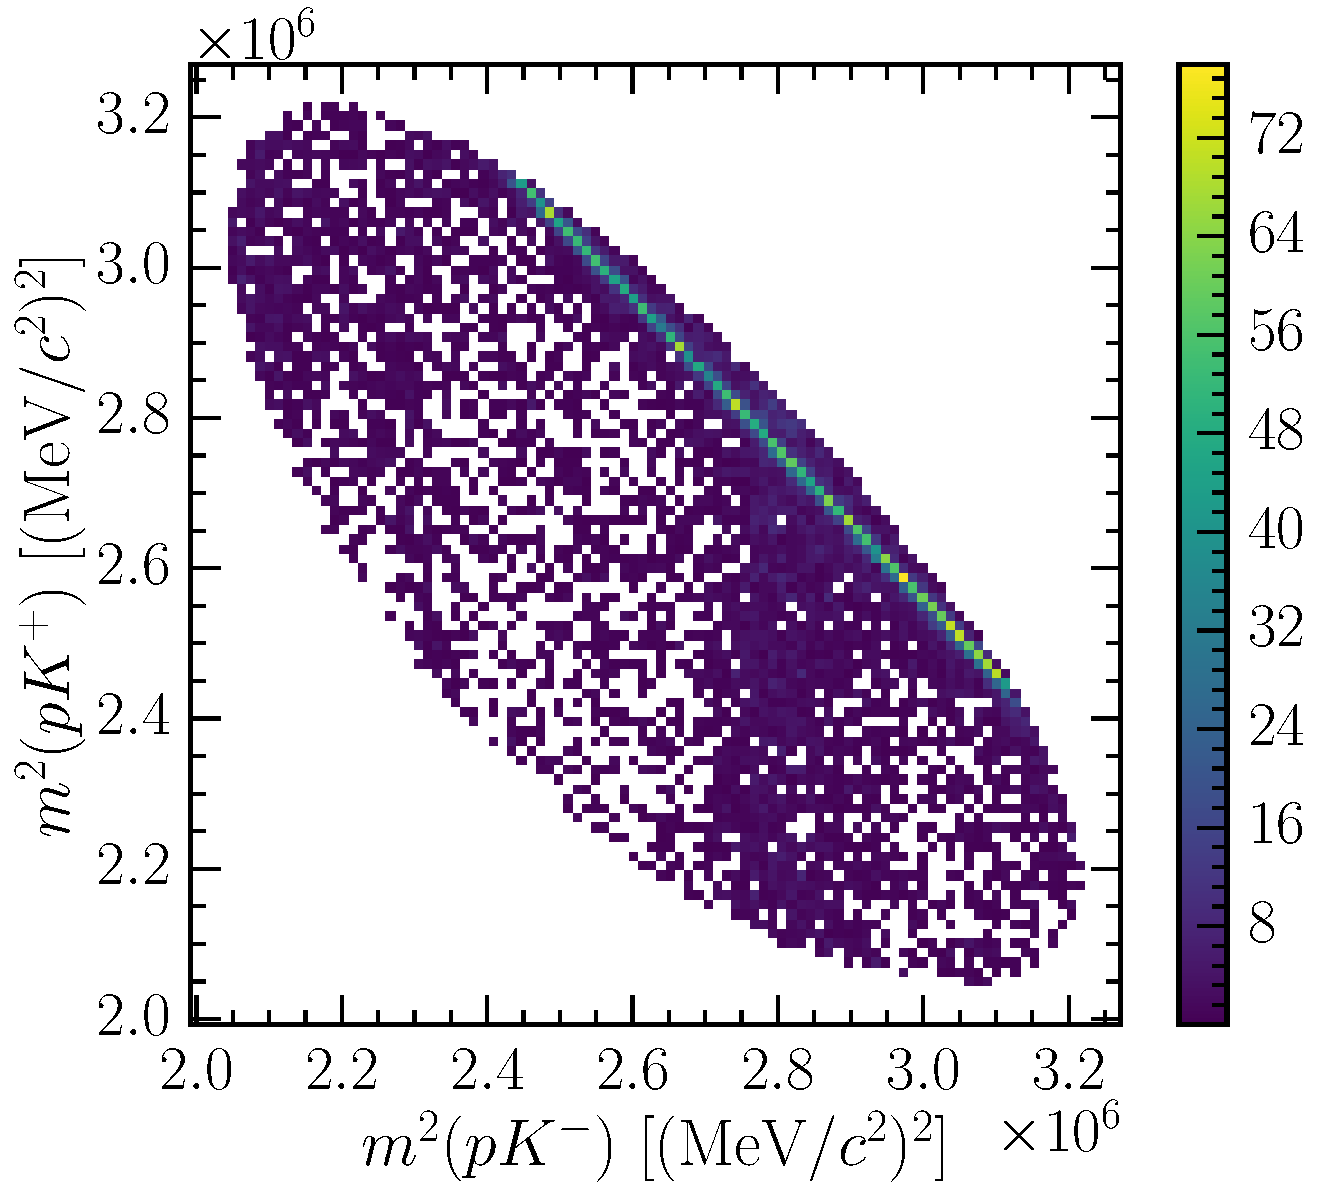
\includegraphics[width=\textwidth]{cpv/phase_space/LcTopKK_2012_MagDown_Lc_p_h1_M-Lc_p_h2_M}
    \label{fig:cpv:phsp:data:pKK:msqphm_msqphp}
  \end{subfigure}
  \begin{subfigure}{0.5\textwidth}
    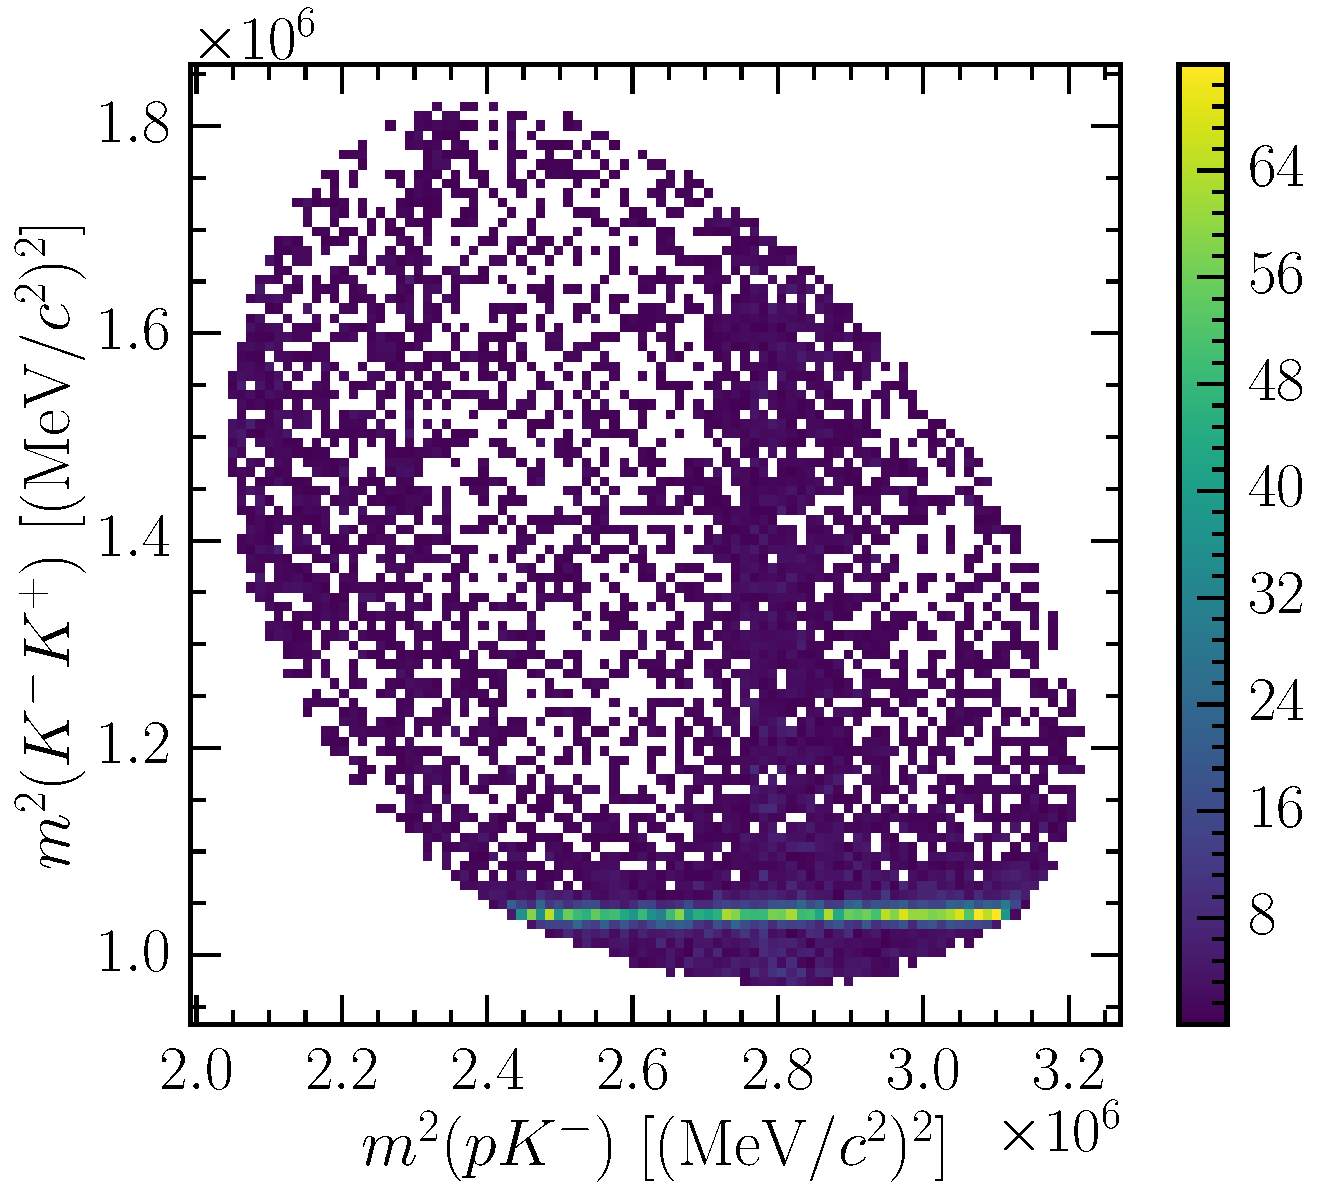
\includegraphics[width=\textwidth]{cpv/phase_space/LcTopKK_2012_MagDown_Lc_p_h1_M-Lc_h1_h2_M}
    \label{fig:cpv:phsp:data:pKK:msqphp_msqhh}
  \end{subfigure}
  \begin{subfigure}{0.5\textwidth}
    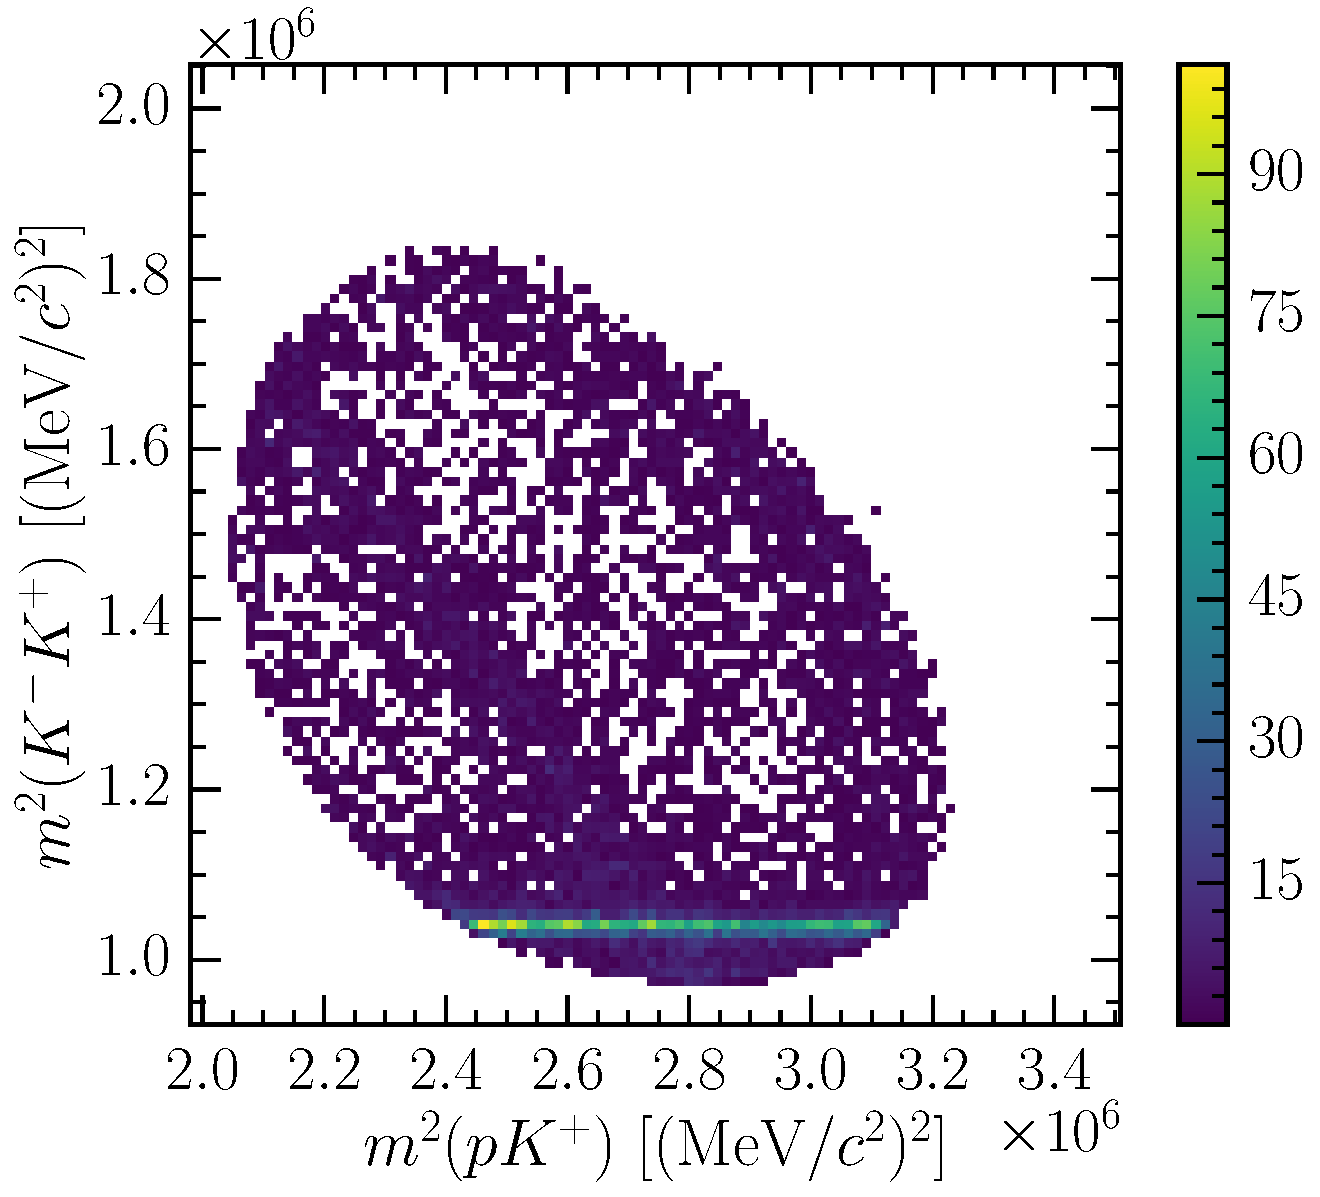
\includegraphics[width=\textwidth]{cpv/phase_space/LcTopKK_2012_MagDown_Lc_p_h2_M-Lc_h1_h2_M}
    \label{fig:cpv:phsp:data:pKK:msqpp_msqhh}
  \end{subfigure}
  \caption{%
    Two dimensional projections of the \LcTopKK\ phase space in the fully 
    selected 2012 magnet down data, weighted by signal sWeights.
    The contents of bins where the sum of signal sWeights is negative are 
    forced to be zero.
  }
  \label{fig:cpv:phsp:data_2D:pKK}
\end{figure}

\begin{figure}
  \centering
  \begin{subfigure}{0.4\textwidth}
    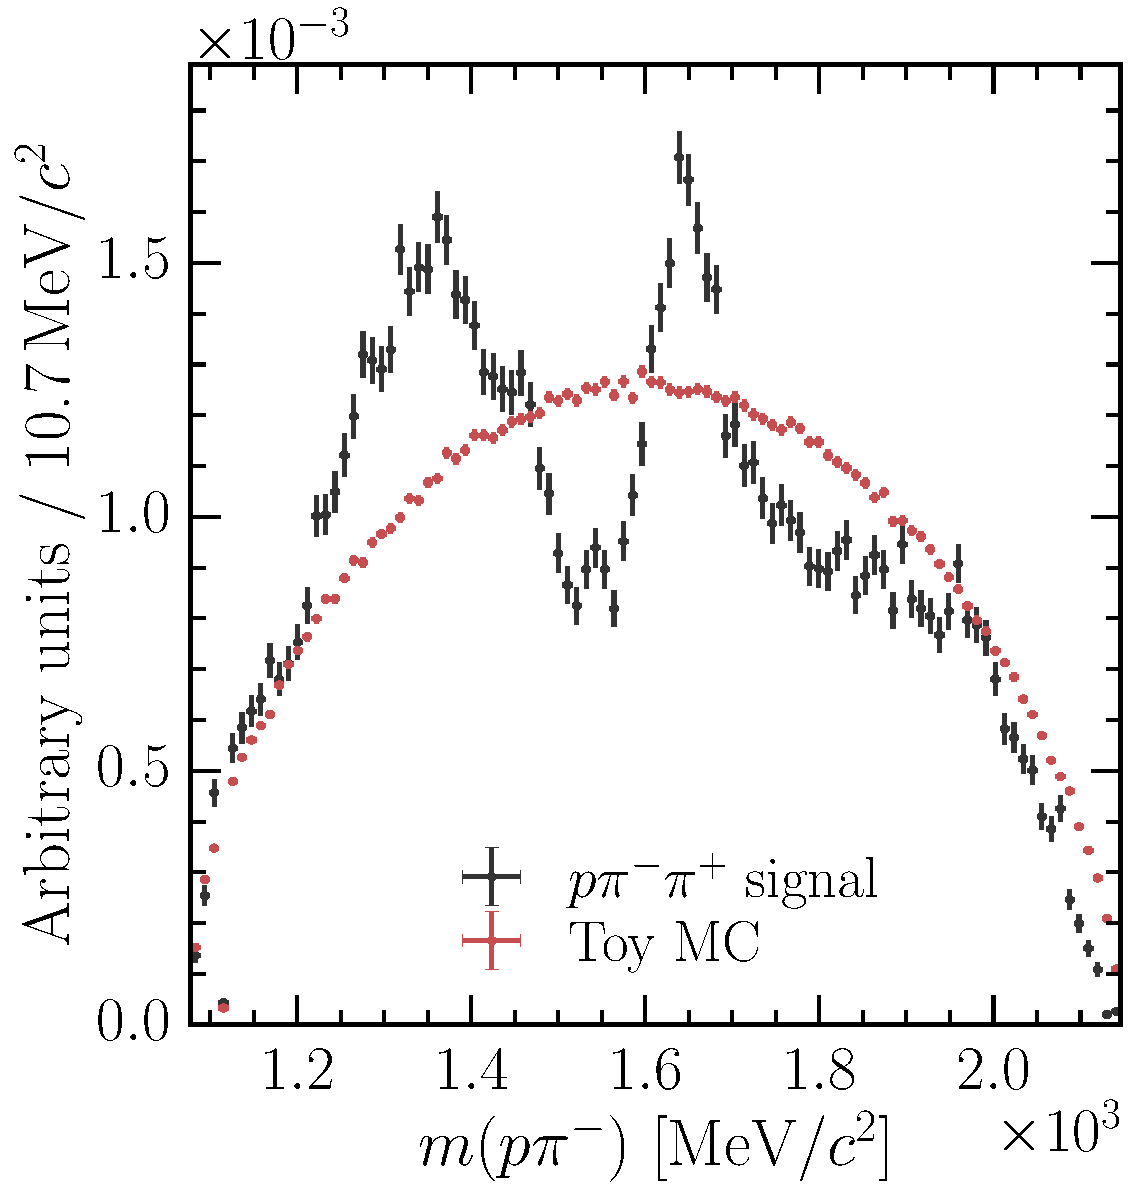
\includegraphics[width=\textwidth]{cpv/phase_space/LcToppipi_2012_MagDown_Lc_p_h1_M}
    \label{fig:cpv:phsp:data:ppipi:msqphm}
  \end{subfigure}
  \begin{subfigure}{0.4\textwidth}
    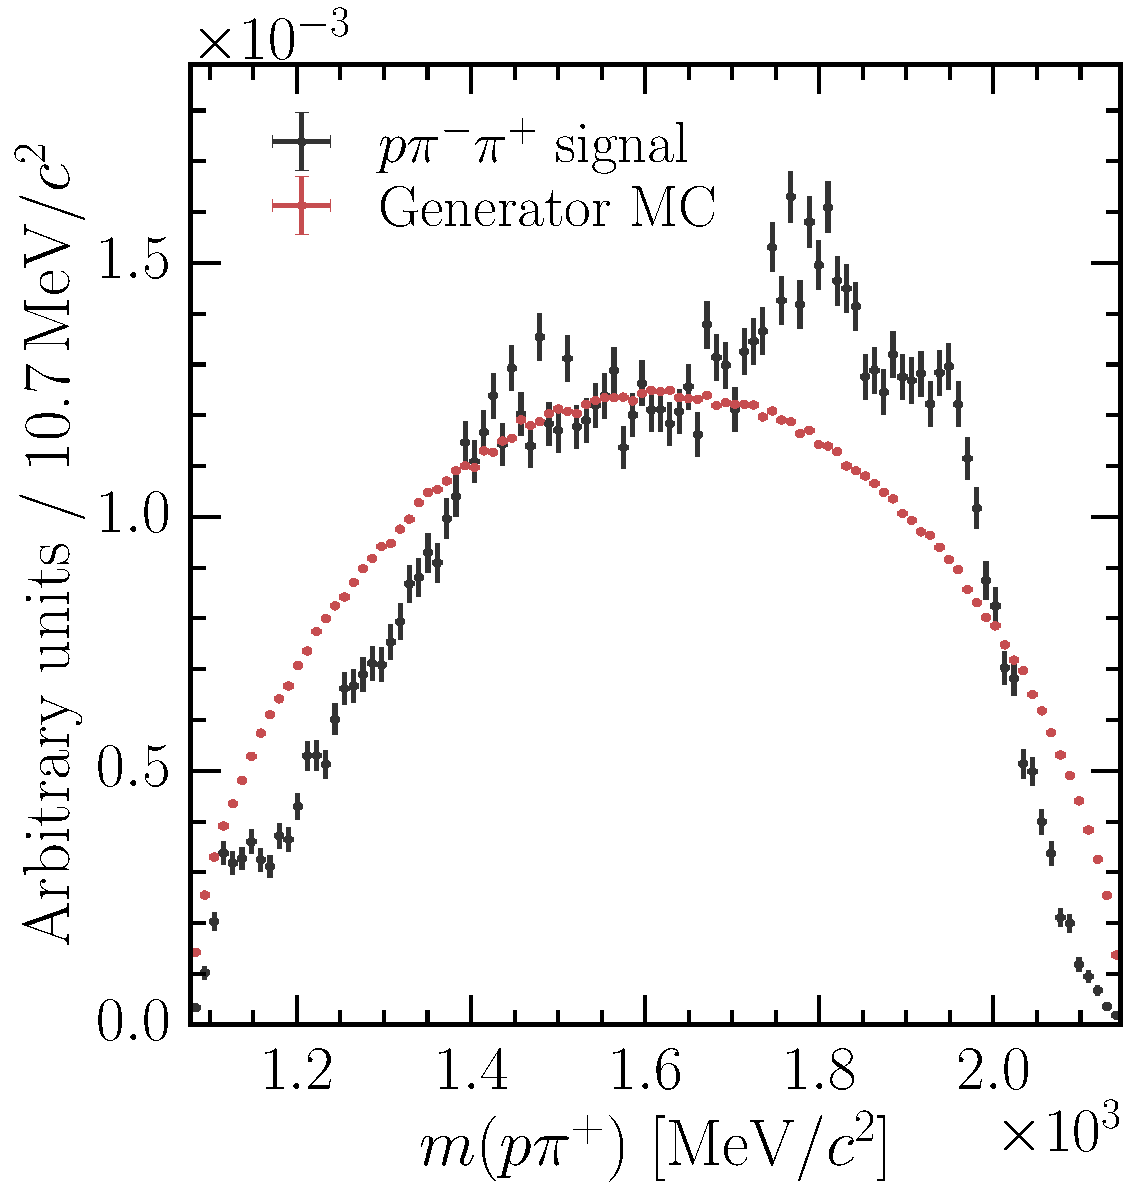
\includegraphics[width=\textwidth]{cpv/phase_space/LcToppipi_2012_MagDown_Lc_p_h2_M}
    \label{fig:cpv:phsp:data:ppipi:msqphp}
  \end{subfigure}
  \begin{subfigure}{0.4\textwidth}
    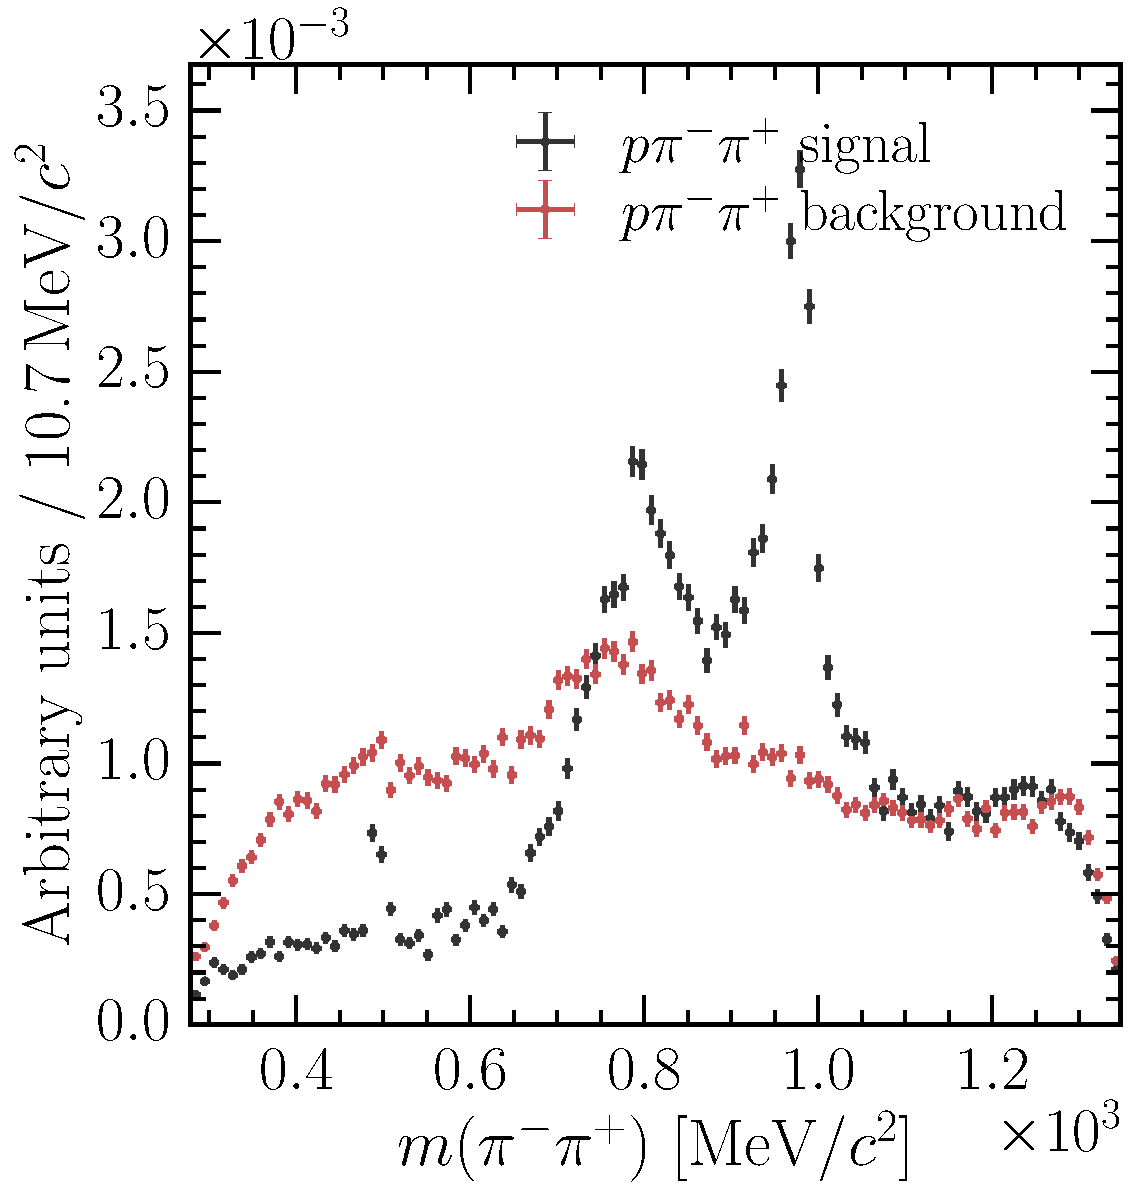
\includegraphics[width=\textwidth]{cpv/phase_space/LcToppipi_2012_MagDown_Lc_h1_h2_M}
    \label{fig:cpv:phsp:data:ppipi:msqhh}
  \end{subfigure}
  \begin{subfigure}{0.4\textwidth}
    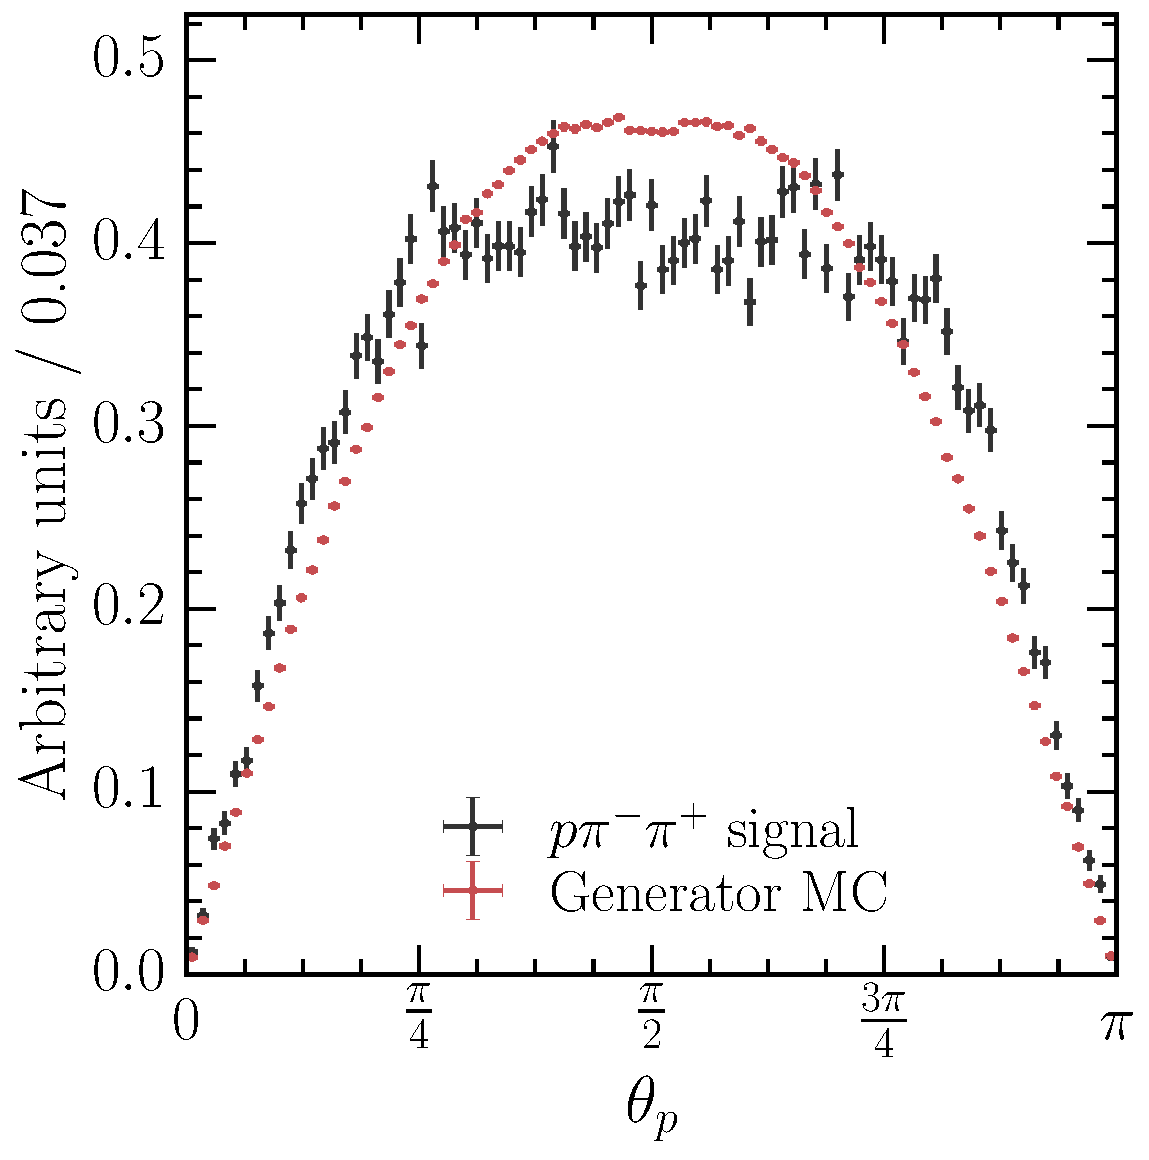
\includegraphics[width=\textwidth]{cpv/phase_space/LcToppipi_2012_MagDown_Lc_phsp_p_theta}
    \label{fig:cpv:phsp:data:ppipi:proton_theta}
  \end{subfigure}
  \begin{subfigure}{0.4\textwidth}
    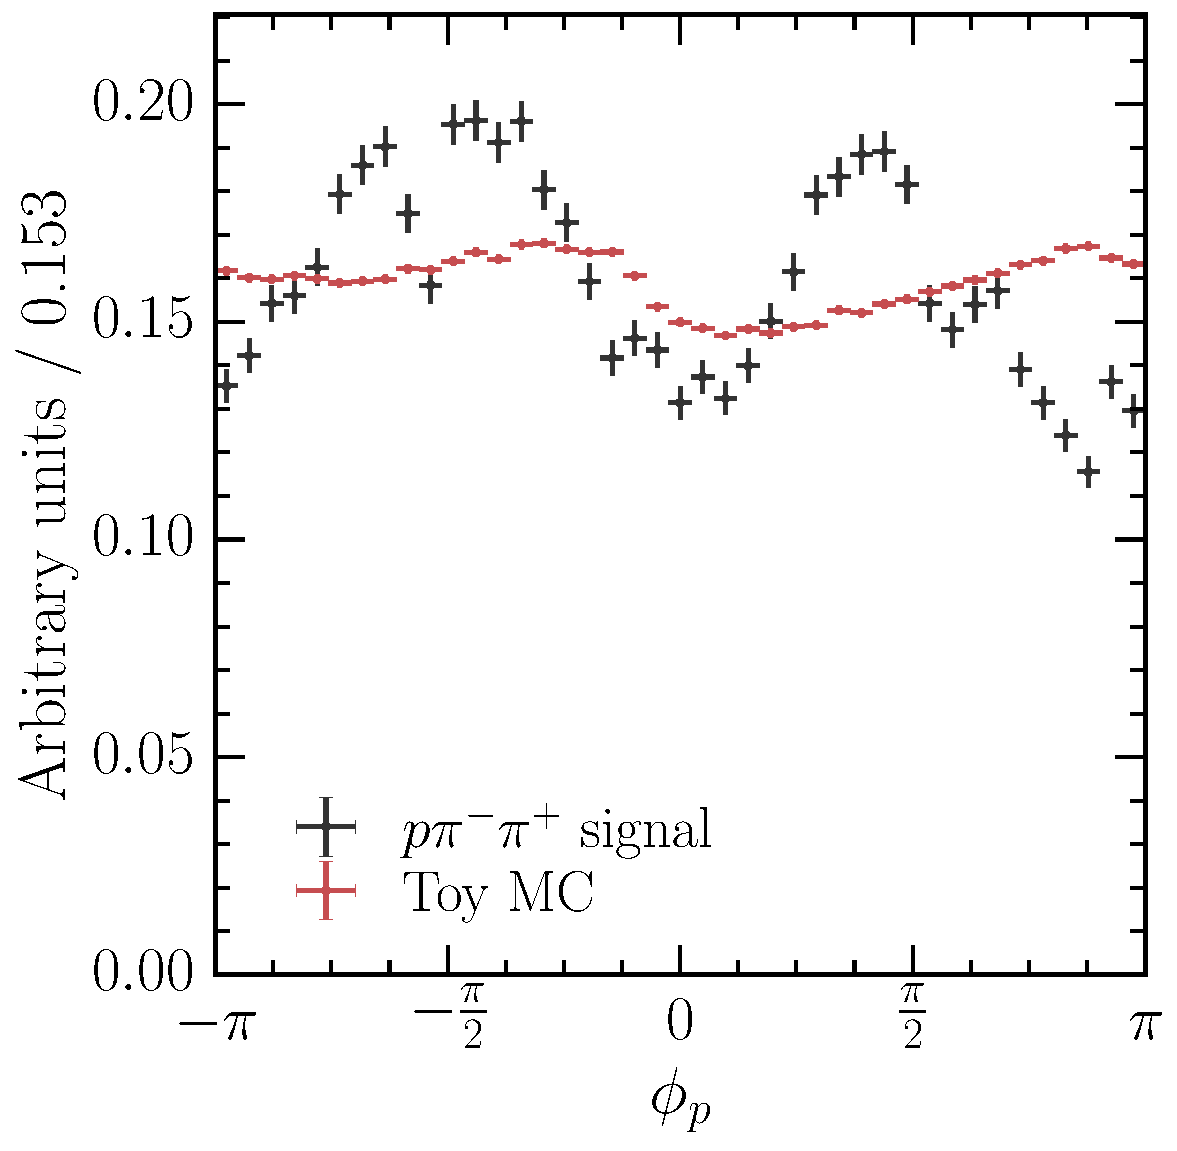
\includegraphics[width=\textwidth]{cpv/phase_space/LcToppipi_2012_MagDown_Lc_phsp_p_phi}
    \label{fig:cpv:phsp:data:ppipi:proton_phi}
  \end{subfigure}
  \begin{subfigure}{0.4\textwidth}
    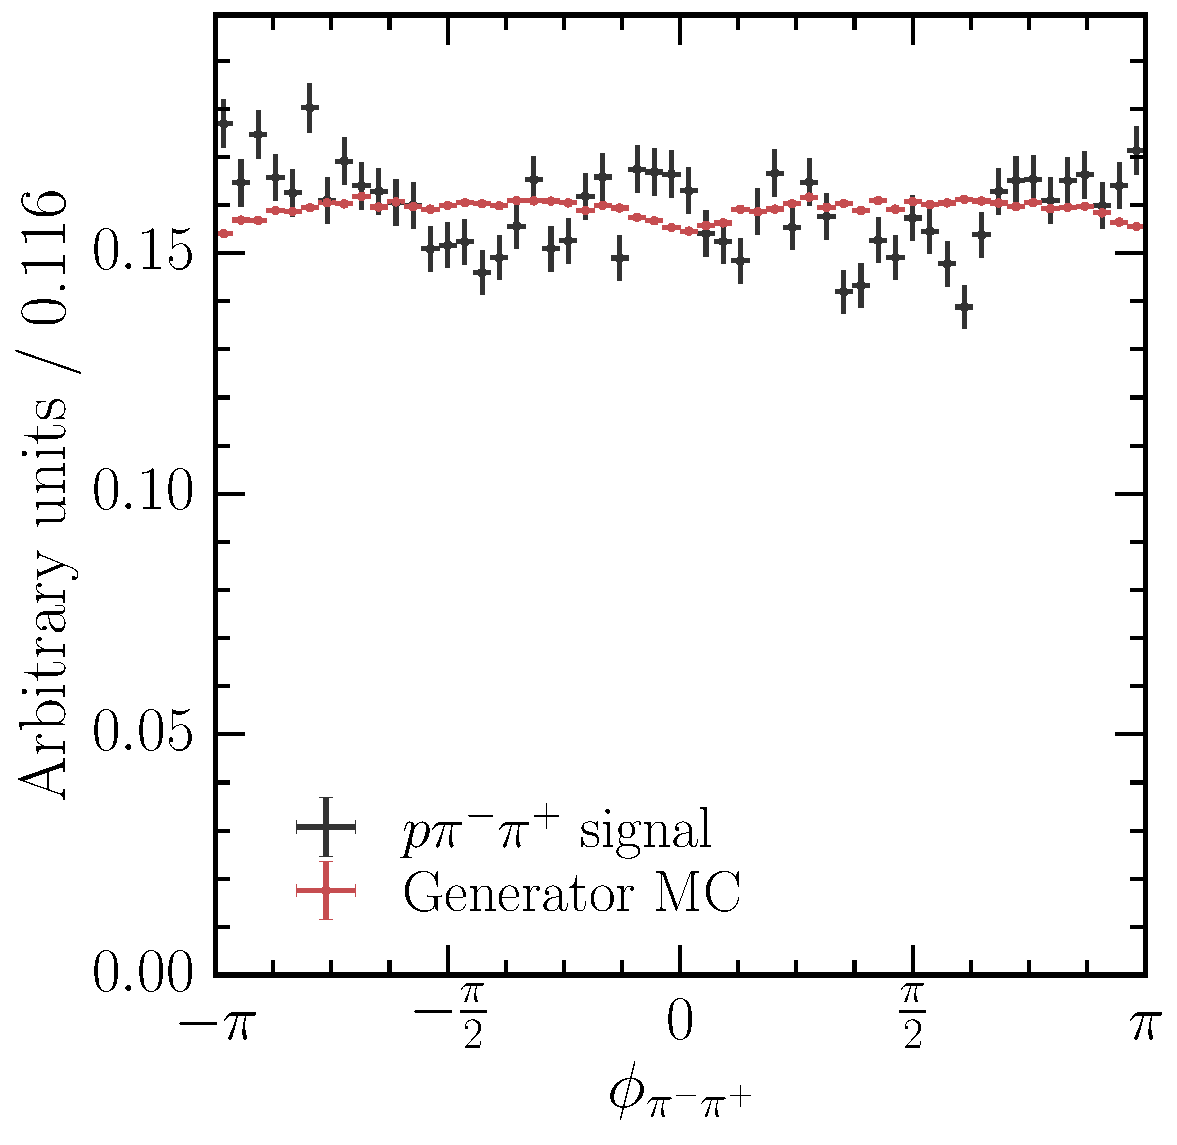
\includegraphics[width=\textwidth]{cpv/phase_space/LcToppipi_2012_MagDown_Lc_phsp_h1_h2_phi}
    \label{fig:cpv:phsp:data:ppipi:h1_h2_phi}
  \end{subfigure}
  \caption{%
    % TODO update these plots to those using the LHCb generator-level MC
    One dimensional projections of the \LcToppipi\ phase space in the fully 
    selected 2012 magnet down data, weighted by signal sWeights, along with the 
    respective one-dimensional projections from the generator-level \ac{MC}, 
    described in \cref{chap:cpv:data:mc:gen}.
  }
  \label{fig:cpv:phsp:data_1D:ppipi}
\end{figure}

\begin{figure}
  \begin{subfigure}{0.5\textwidth}
    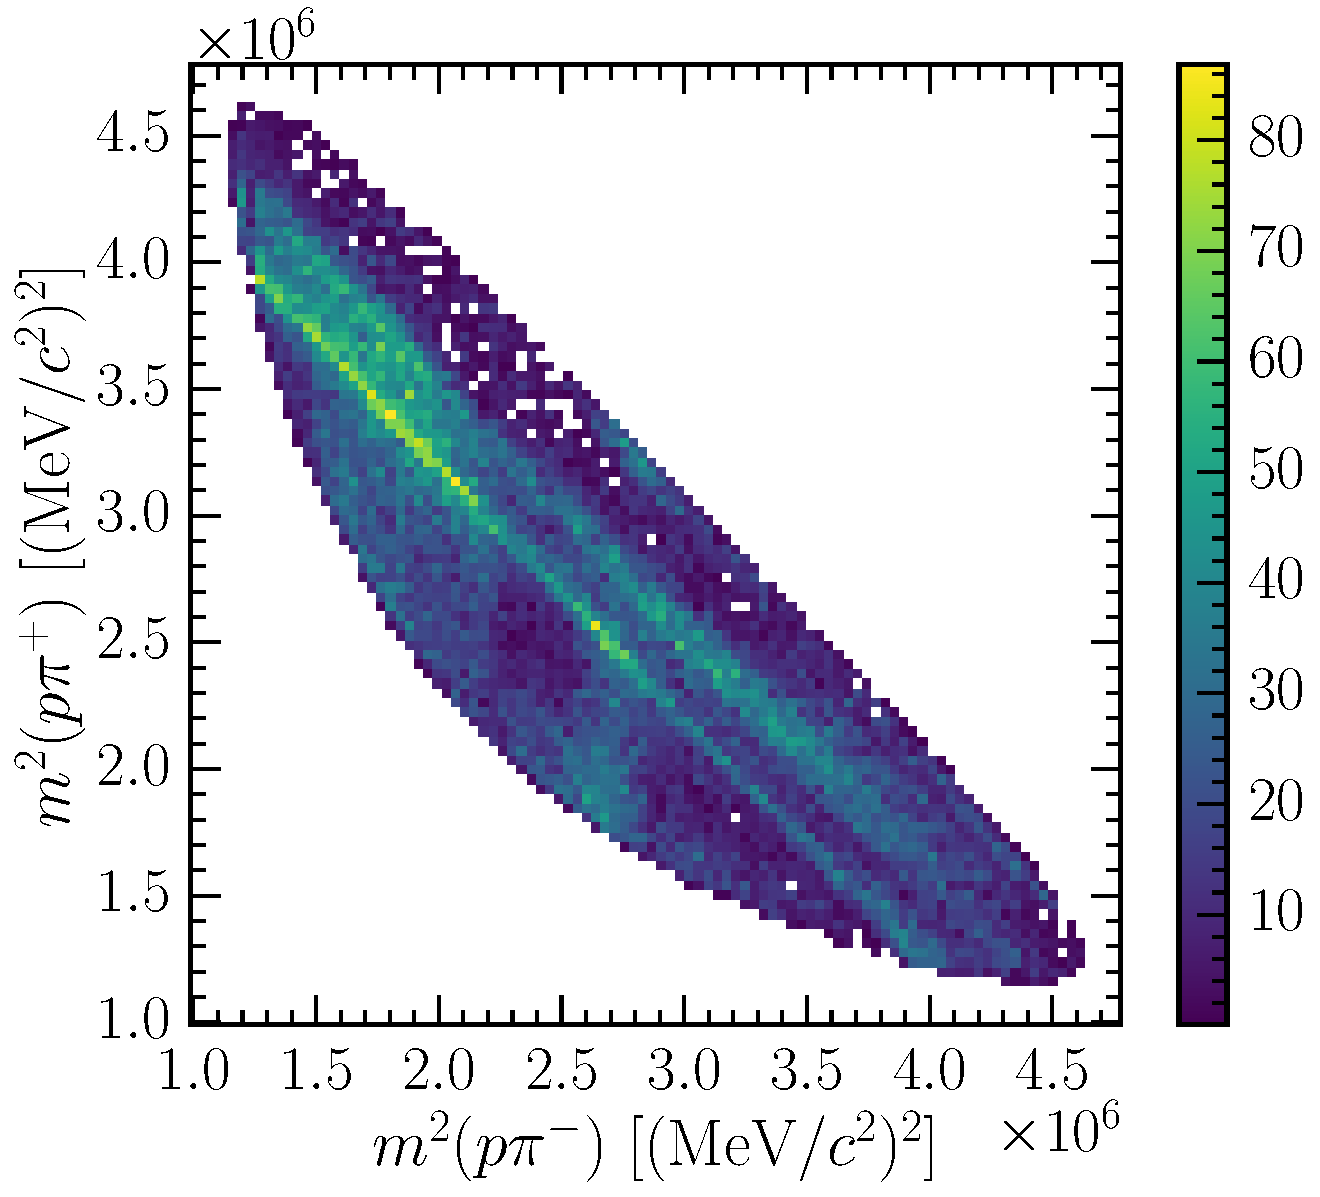
\includegraphics[width=\textwidth]{cpv/phase_space/LcToppipi_2012_MagDown_Lc_p_h1_M-Lc_p_h2_M}
    \label{fig:cpv:phsp:data:ppipi:msqphm_msqphp}
    \caption{\msqphm-\msqphp}
  \end{subfigure}
  \begin{subfigure}{0.5\textwidth}
    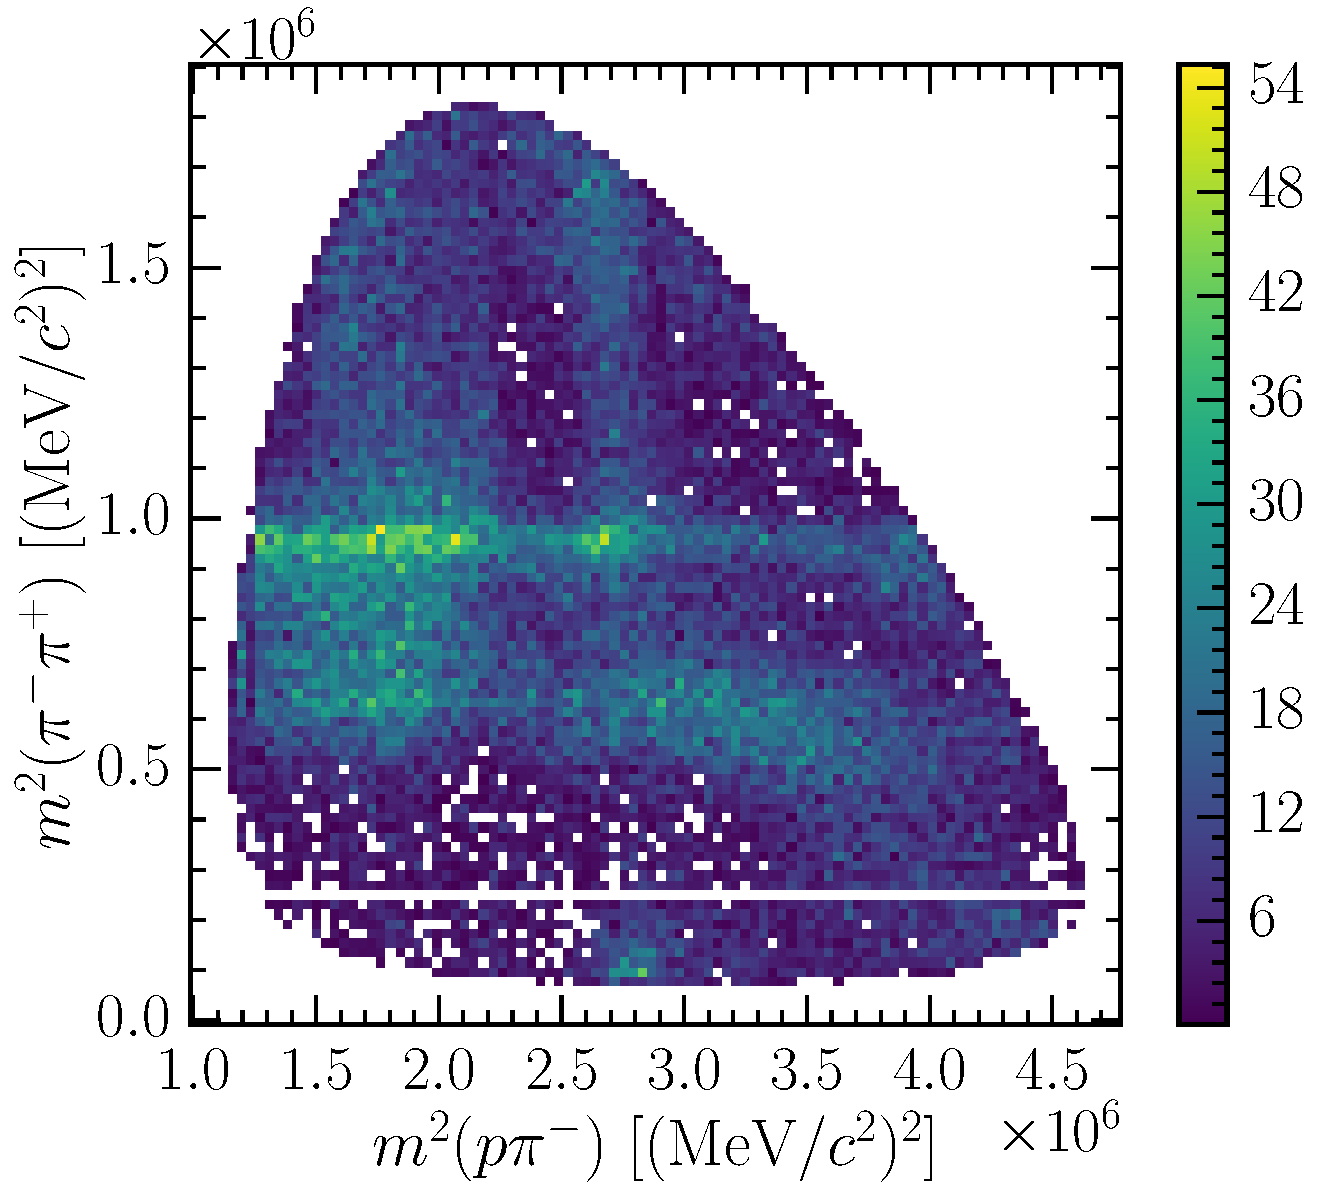
\includegraphics[width=\textwidth]{cpv/phase_space/LcToppipi_2012_MagDown_Lc_p_h1_M-Lc_h1_h2_M}
    \label{fig:cpv:phsp:data:ppipi:msqphp_msqhh}
    \caption{\msqphm-\msqhh}
  \end{subfigure}
  \begin{subfigure}{0.5\textwidth}
    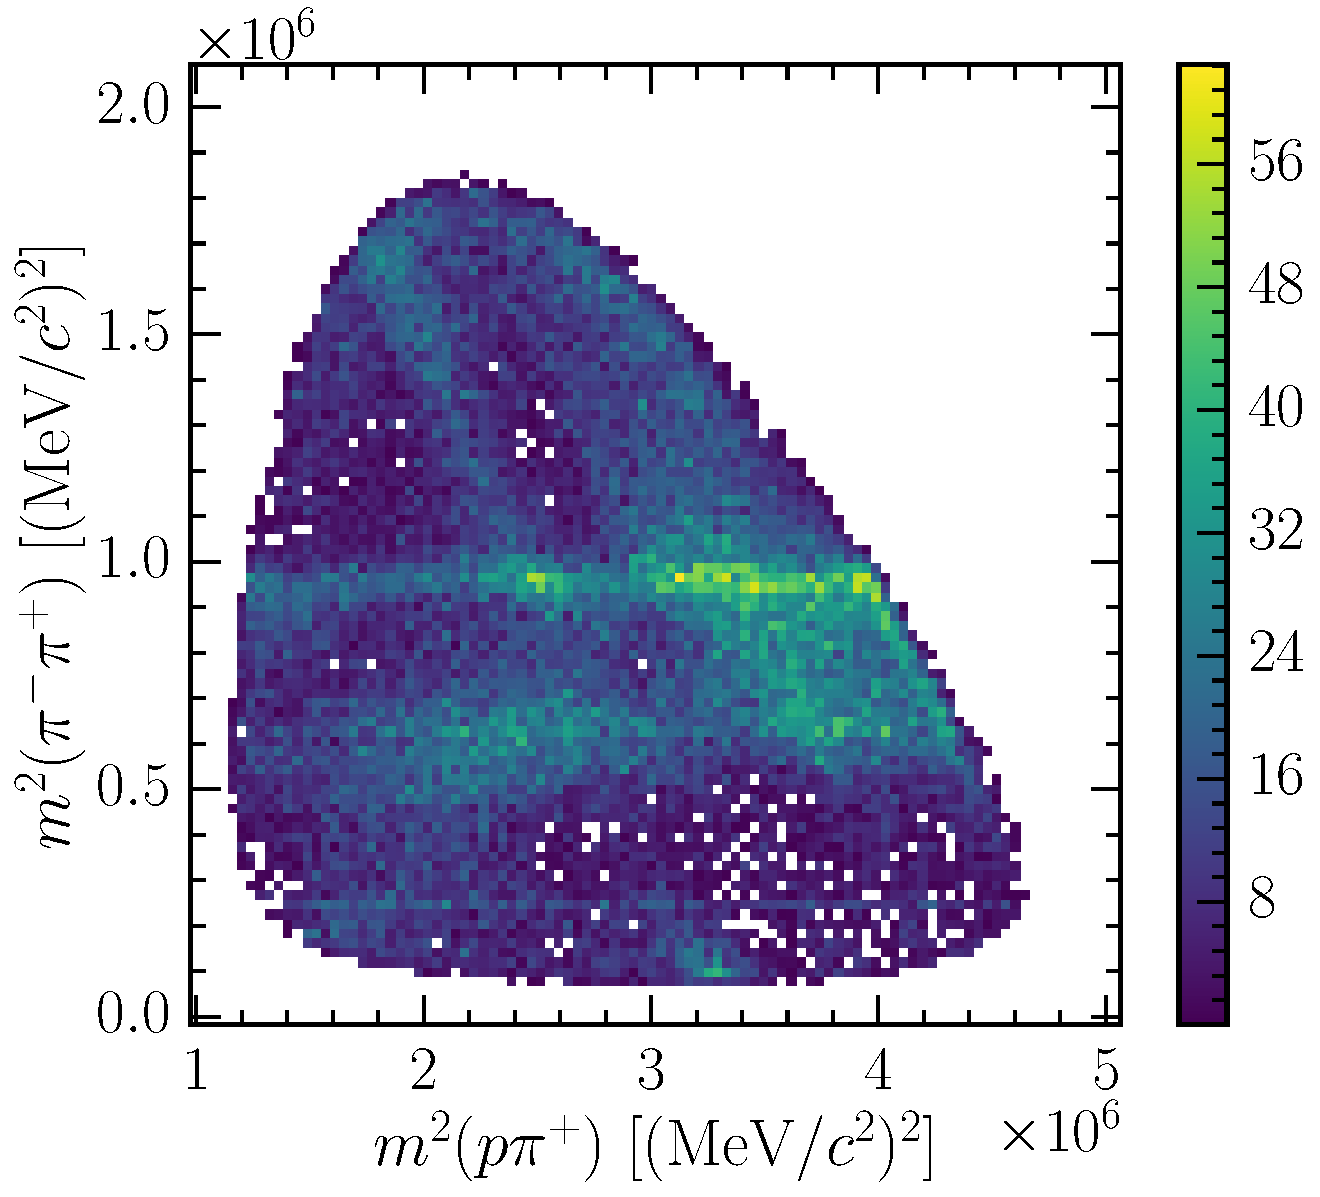
\includegraphics[width=\textwidth]{cpv/phase_space/LcToppipi_2012_MagDown_Lc_p_h2_M-Lc_h1_h2_M}
    \label{fig:cpv:phsp:data:ppipi:msqpp_msqhh}
    \caption{\msqphp-\msqhh}
  \end{subfigure}
  \caption{%
    Two dimensional projections of the \LcToppipi\ phase space in the fully 
    selected 2012 magnet down data, weighted by signal sWeights.
    The contents of bins where the sum of signal sWeights is negative are 
    forced to be zero.
  }
  \label{fig:cpv:phsp:data_2D:ppipi}
\end{figure}

\begin{figure}
  \centering

  \begin{subfigure}{0.25\textwidth}
    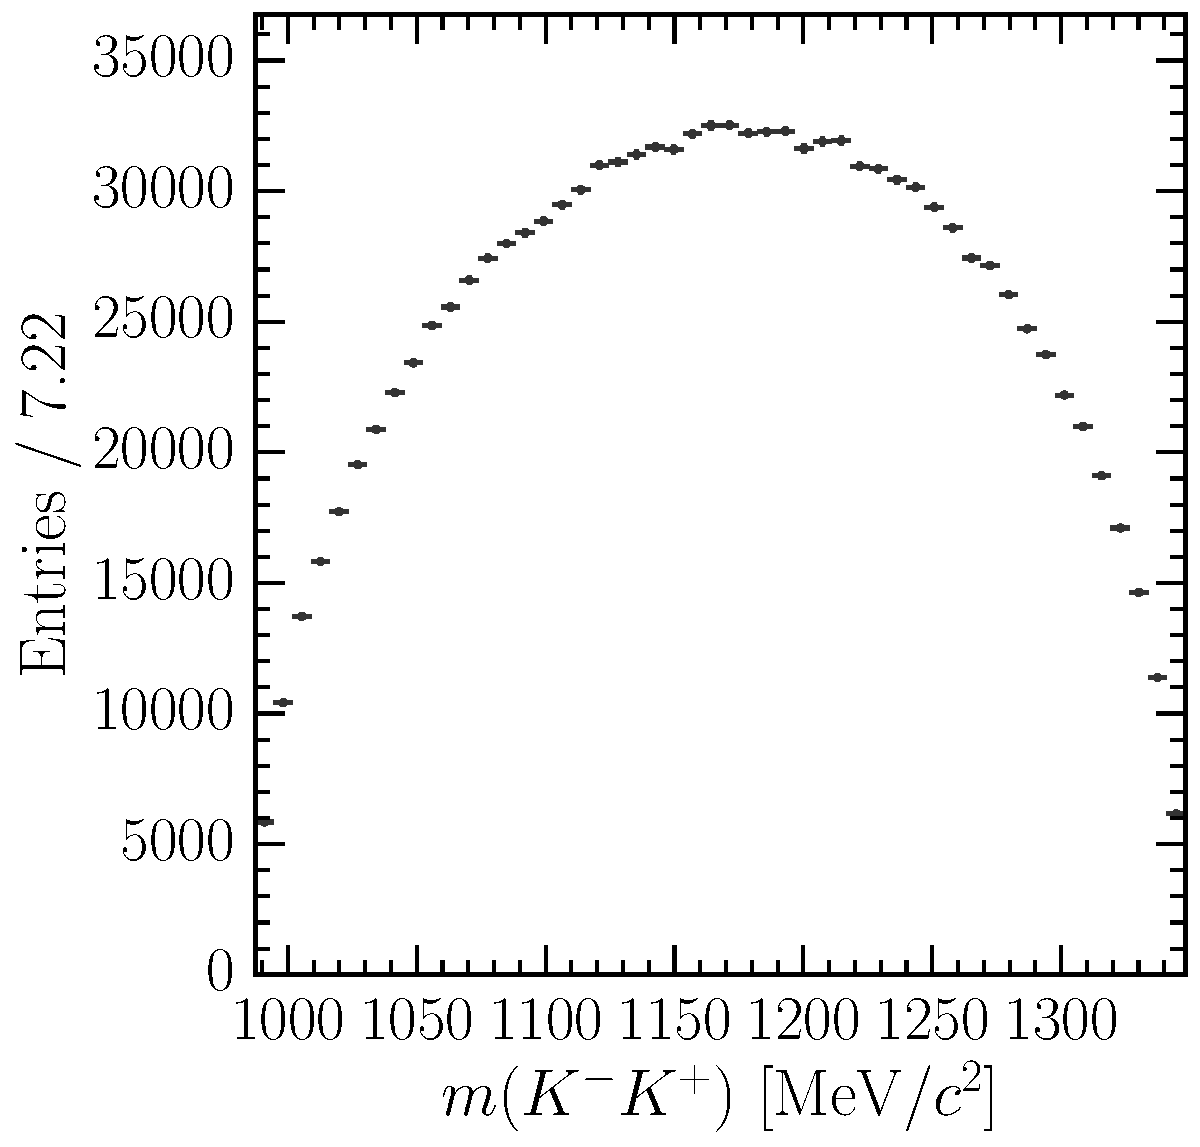
\includegraphics[width=\textwidth]{cpv/phase_space/LcTopKK_2012_MagDown_Lc_h1_h2_M_before_selection}
    \label{fig:cpv:phsp:effs:pKK:Lc_h1_h2_M:before}
  \end{subfigure}
  \begin{subfigure}{0.25\textwidth}
    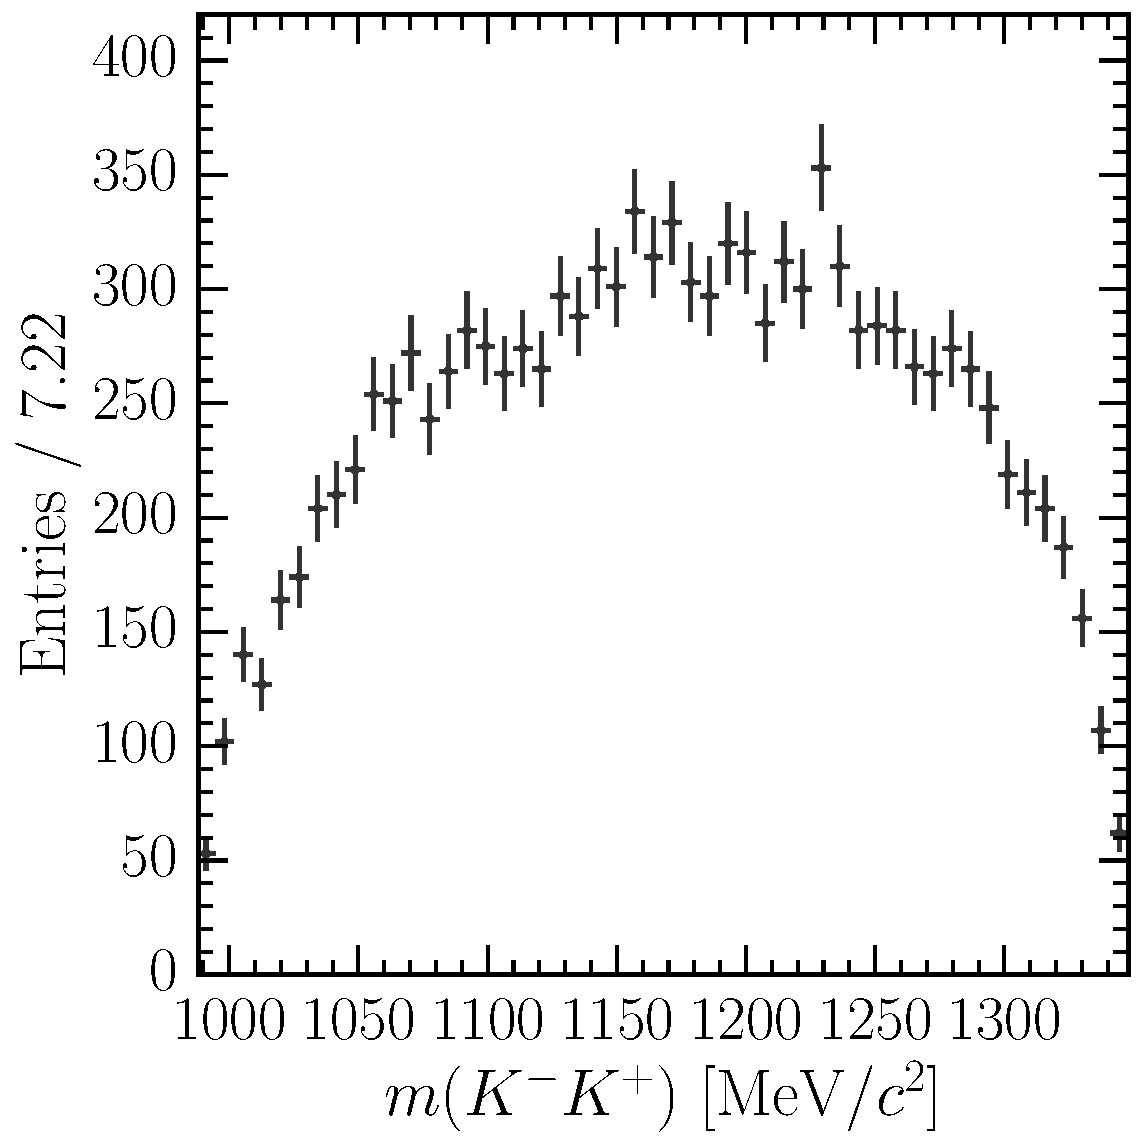
\includegraphics[width=\textwidth]{cpv/phase_space/LcTopKK_2012_MagDown_Lc_h1_h2_M_after_selection}
    \label{fig:cpv:phsp:effs:pKK:Lc_h1_h2_M:after}
  \end{subfigure}
  \begin{subfigure}{0.25\textwidth}
    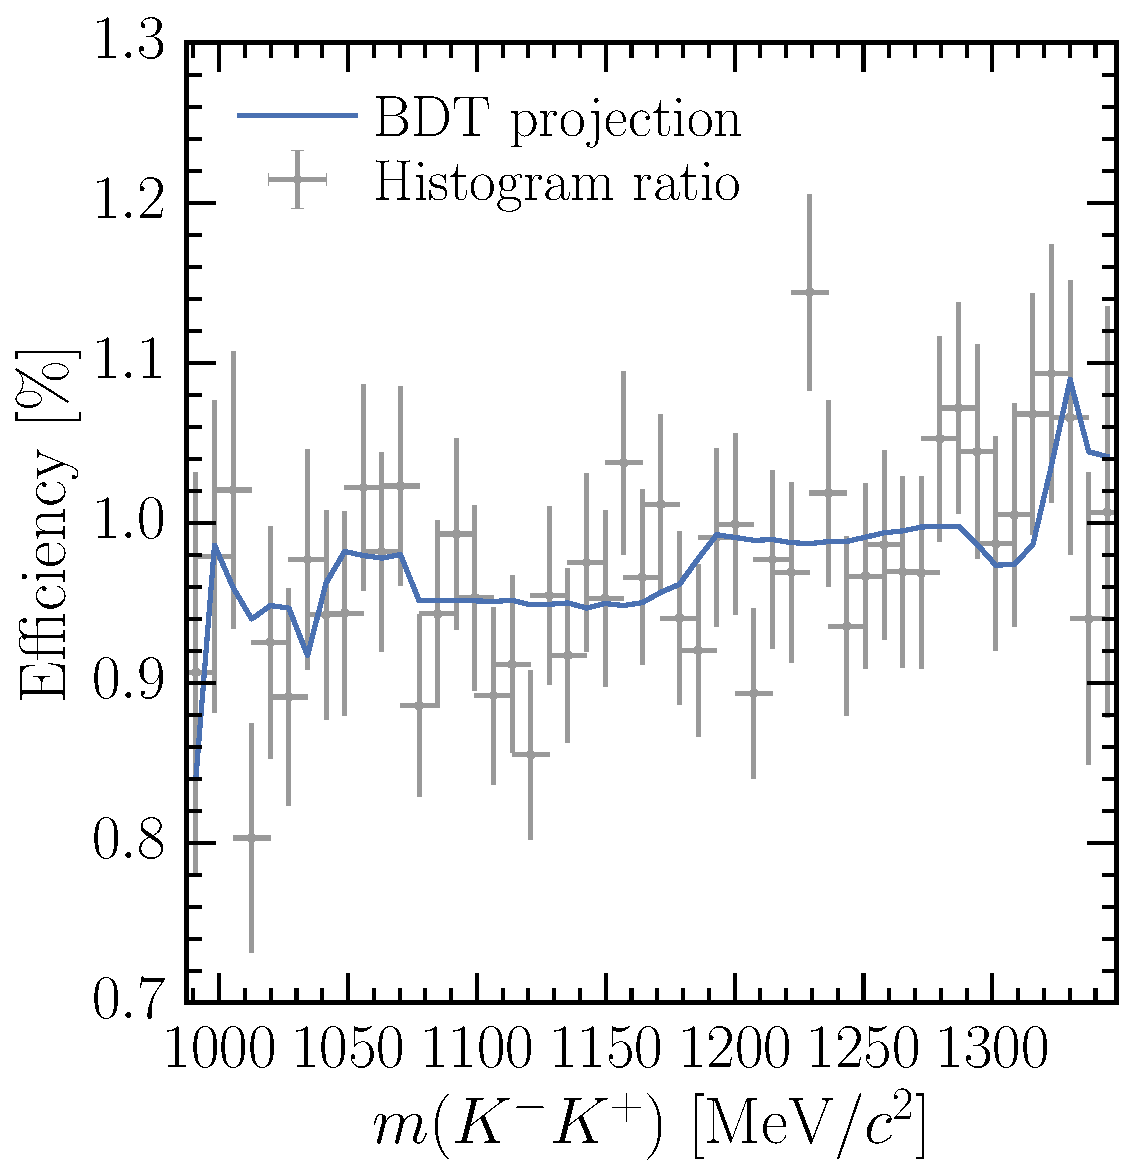
\includegraphics[width=\textwidth]{cpv/phase_space/LcTopKK_2012_MagDown_Lc_h1_h2_M_efficiency}
    \label{fig:cpv:phsp:effs:pKK:Lc_h1_h2_M:eff}
  \end{subfigure}

  \begin{subfigure}{0.25\textwidth}
    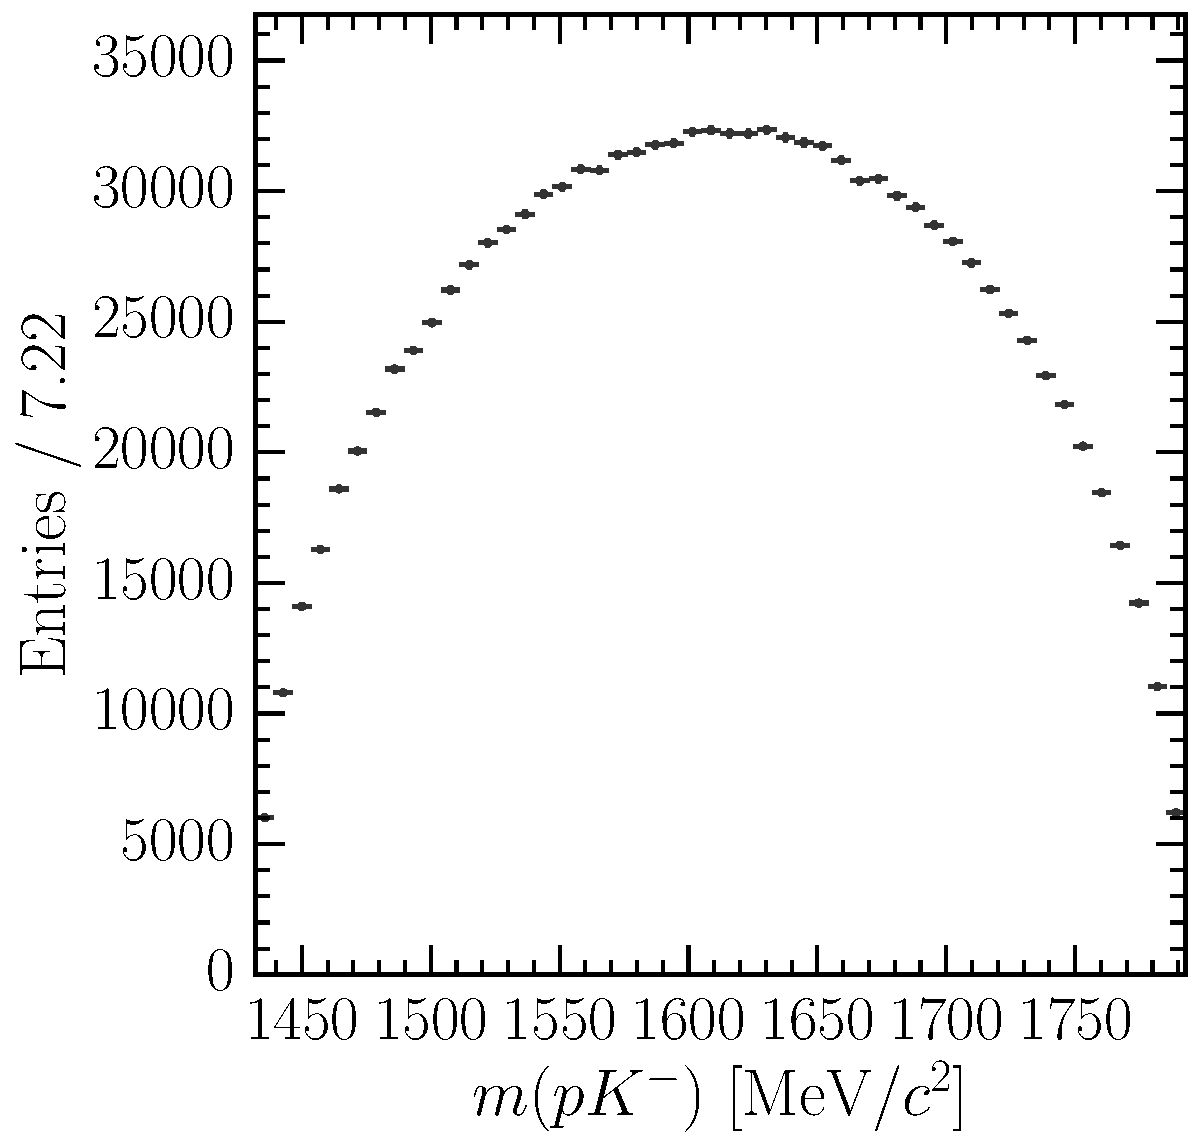
\includegraphics[width=\textwidth]{cpv/phase_space/LcTopKK_2012_MagDown_Lc_p_h1_M_before_selection}
    \label{fig:cpv:phsp:effs:pKK:Lc_p_h1_M:before}
  \end{subfigure}
  \begin{subfigure}{0.25\textwidth}
    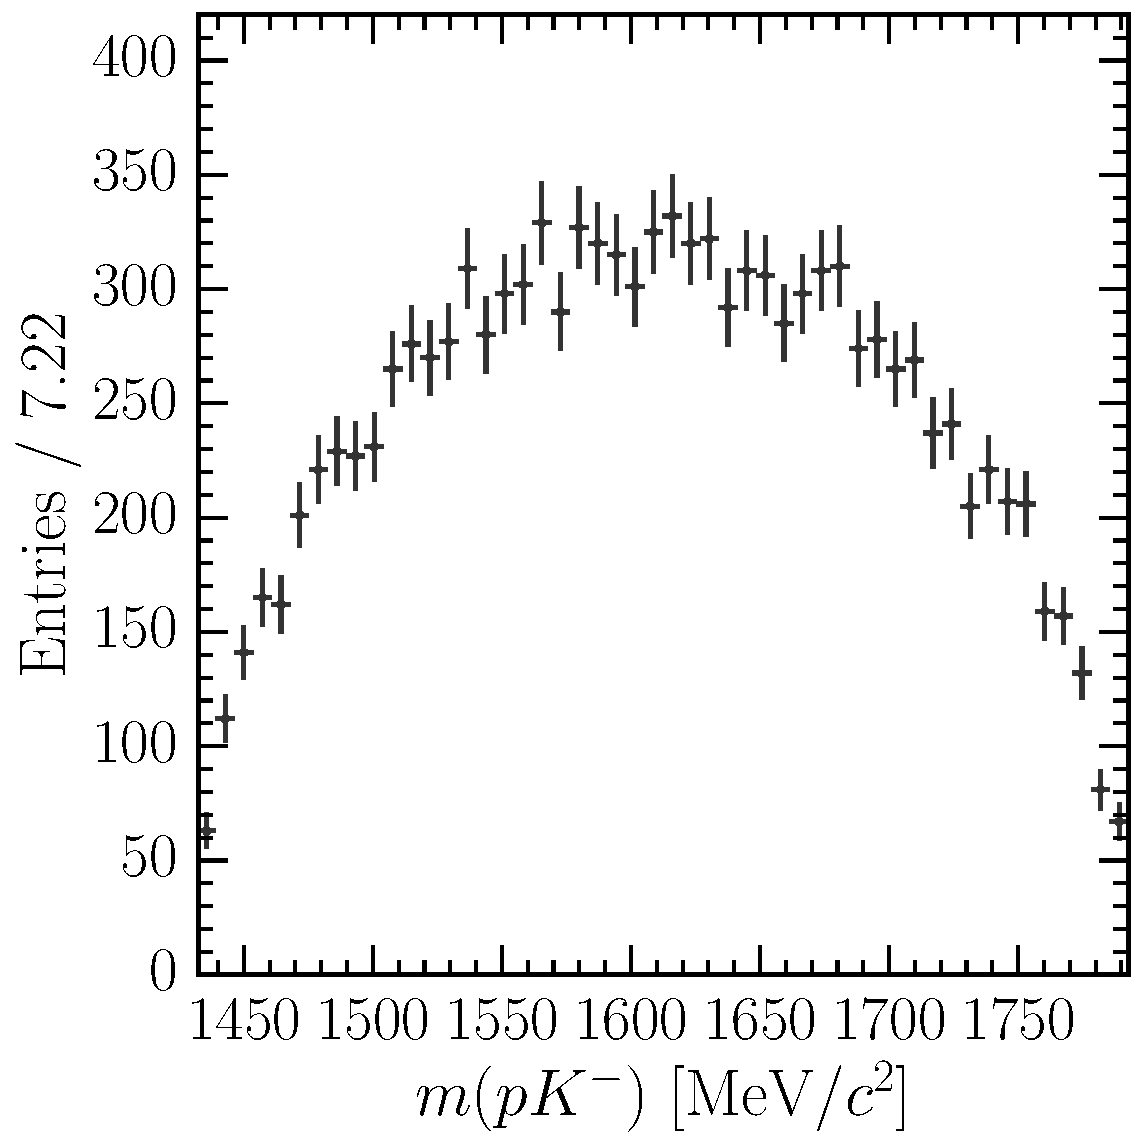
\includegraphics[width=\textwidth]{cpv/phase_space/LcTopKK_2012_MagDown_Lc_p_h1_M_after_selection}
    \label{fig:cpv:phsp:effs:pKK:Lc_p_h1_M:after}
  \end{subfigure}
  \begin{subfigure}{0.25\textwidth}
    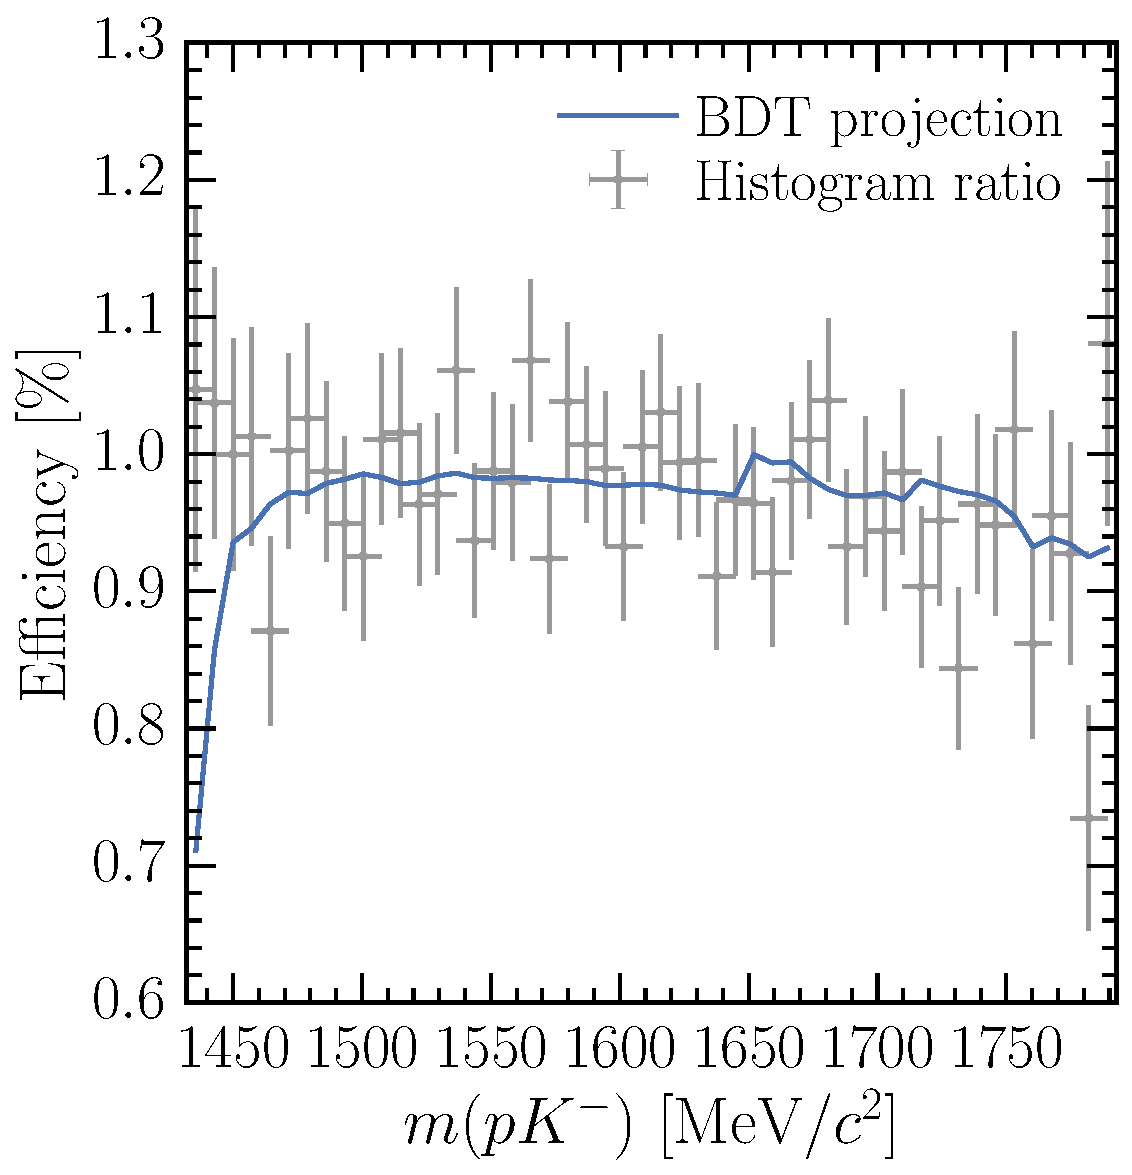
\includegraphics[width=\textwidth]{cpv/phase_space/LcTopKK_2012_MagDown_Lc_p_h1_M_efficiency}
    \label{fig:cpv:phsp:effs:pKK:Lc_p_h1_M:eff}
  \end{subfigure}

  \begin{subfigure}{0.25\textwidth}
    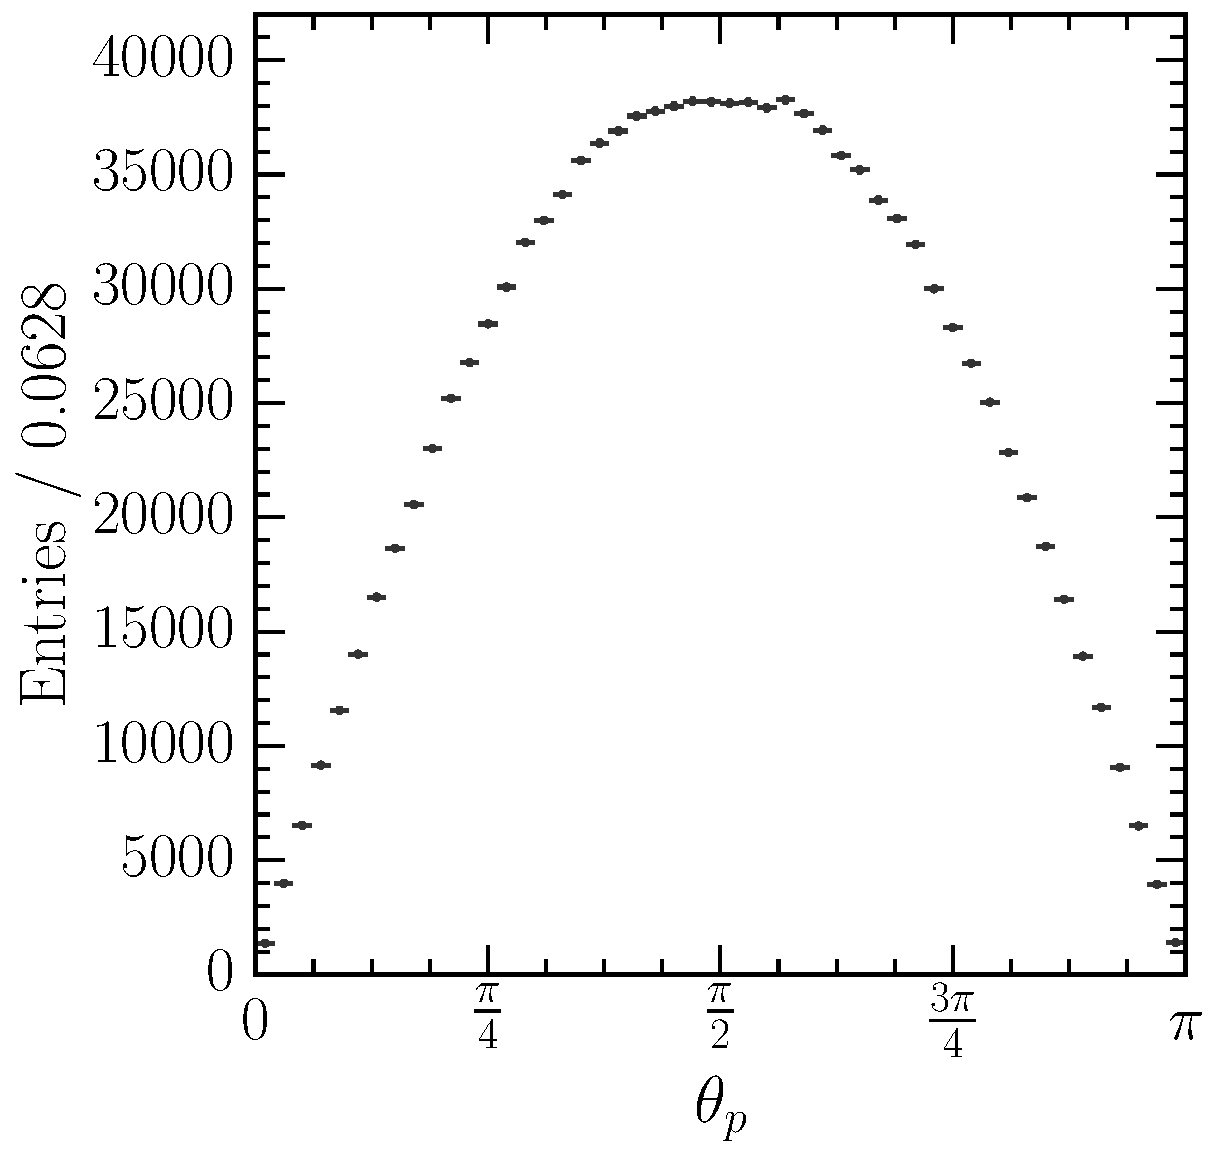
\includegraphics[width=\textwidth]{cpv/phase_space/LcTopKK_2012_MagDown_Lc_phsp_p_theta_before_selection}
    \label{fig:cpv:phsp:effs:pKK:Lc_phsp_p_theta:before}
  \end{subfigure}
  \begin{subfigure}{0.25\textwidth}
    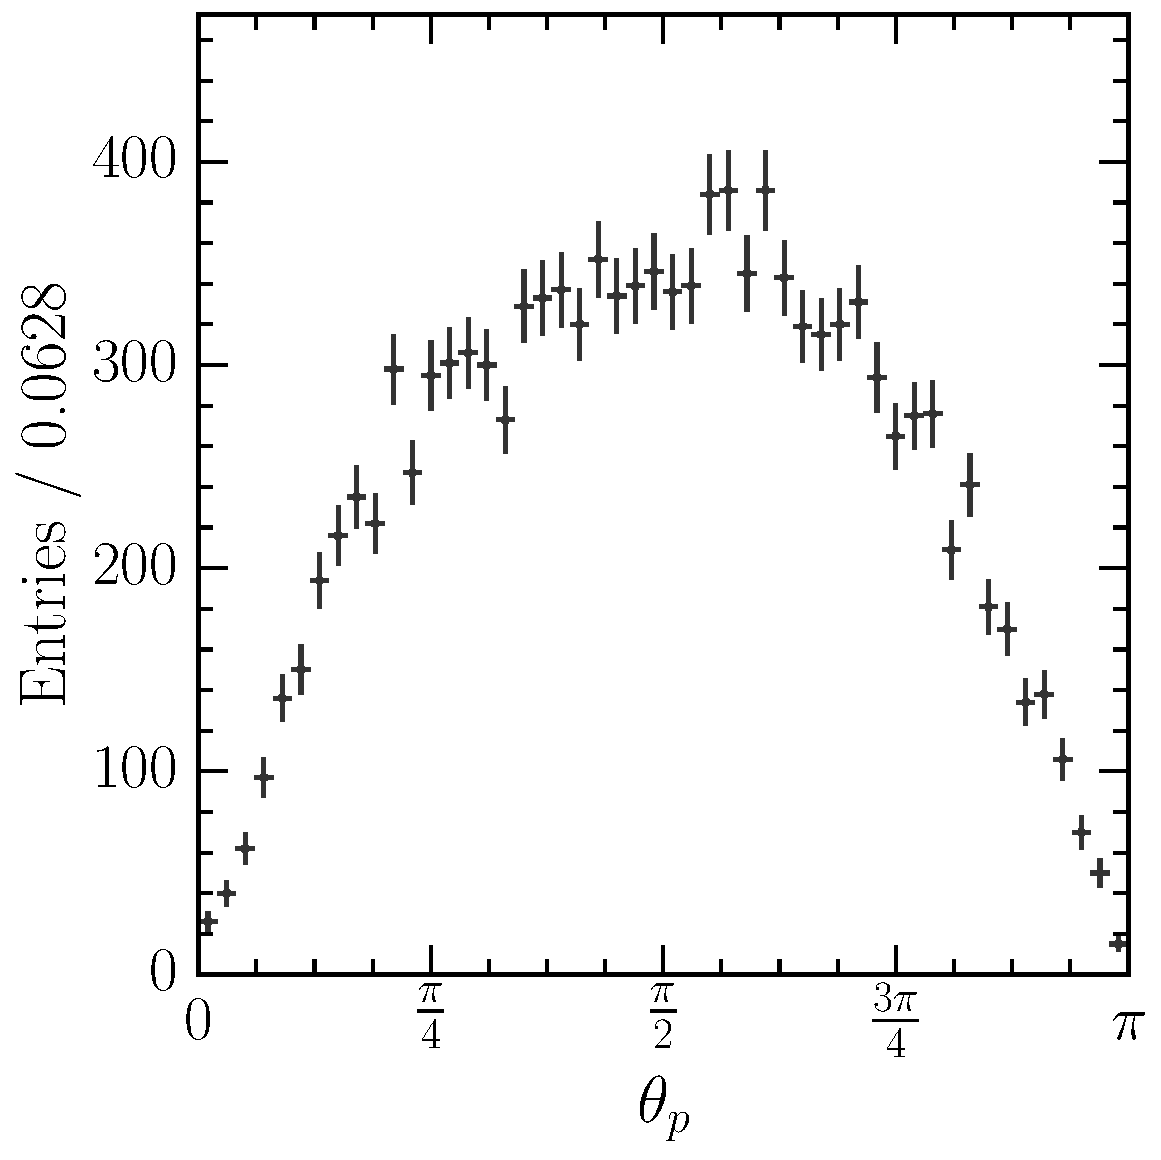
\includegraphics[width=\textwidth]{cpv/phase_space/LcTopKK_2012_MagDown_Lc_phsp_p_theta_after_selection}
    \label{fig:cpv:phsp:effs:pKK:Lc_phsp_p_theta:after}
  \end{subfigure}
  \begin{subfigure}{0.25\textwidth}
    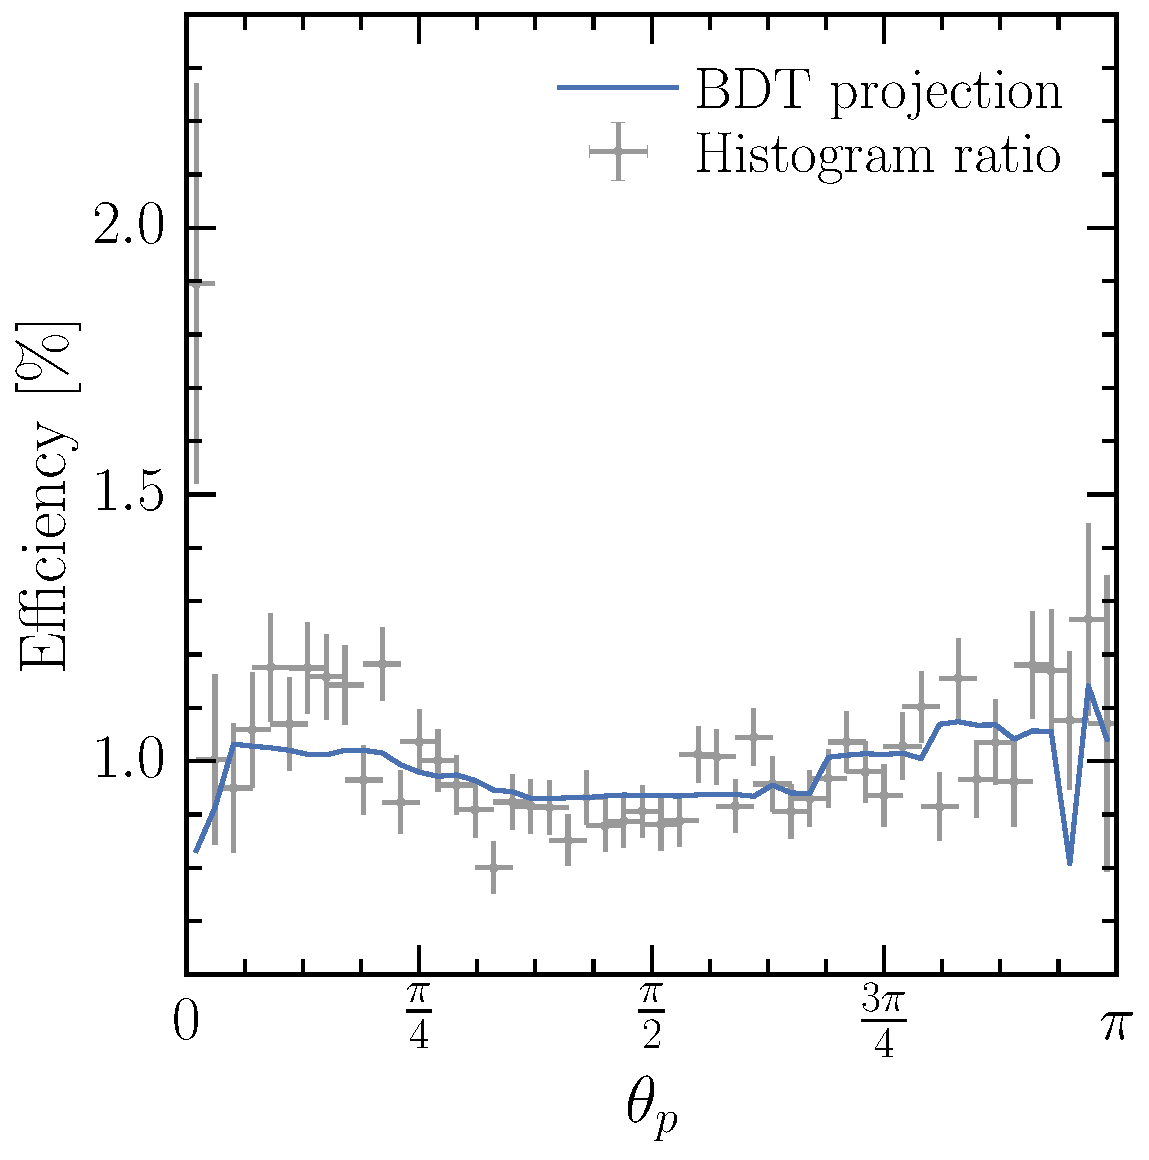
\includegraphics[width=\textwidth]{cpv/phase_space/LcTopKK_2012_MagDown_Lc_phsp_p_theta_efficiency}
    \label{fig:cpv:phsp:effs:pKK:Lc_phsp_p_theta:eff}
  \end{subfigure}

  \begin{subfigure}{0.25\textwidth}
    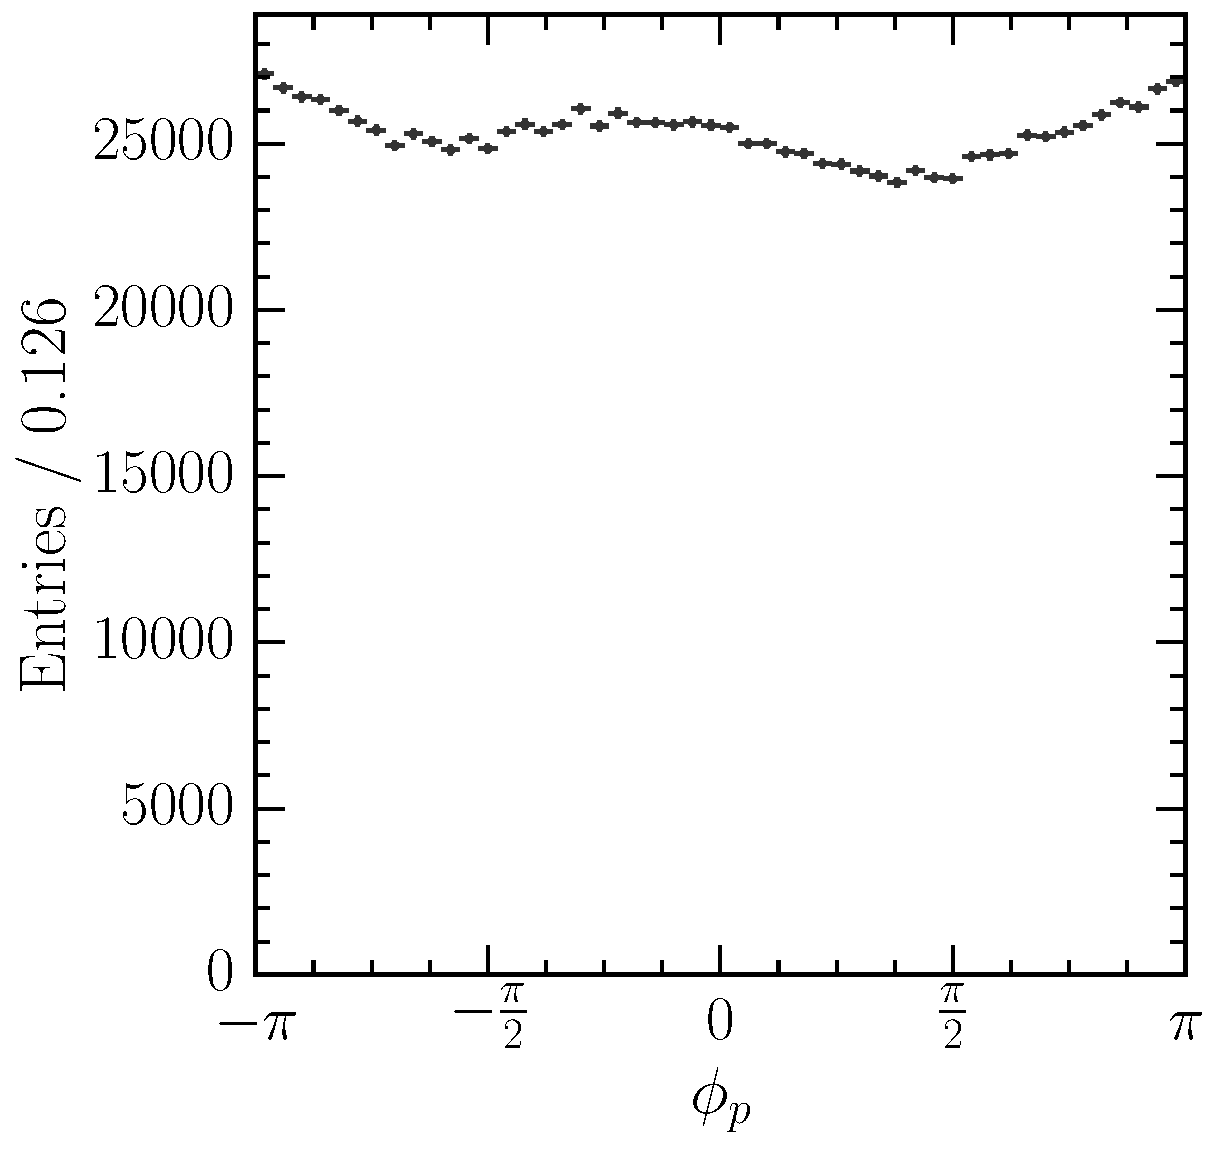
\includegraphics[width=\textwidth]{cpv/phase_space/LcTopKK_2012_MagDown_Lc_phsp_p_phi_before_selection}
    \label{fig:cpv:phsp:effs:pKK:Lc_phsp_p_phi:before}
  \end{subfigure}
  \begin{subfigure}{0.25\textwidth}
    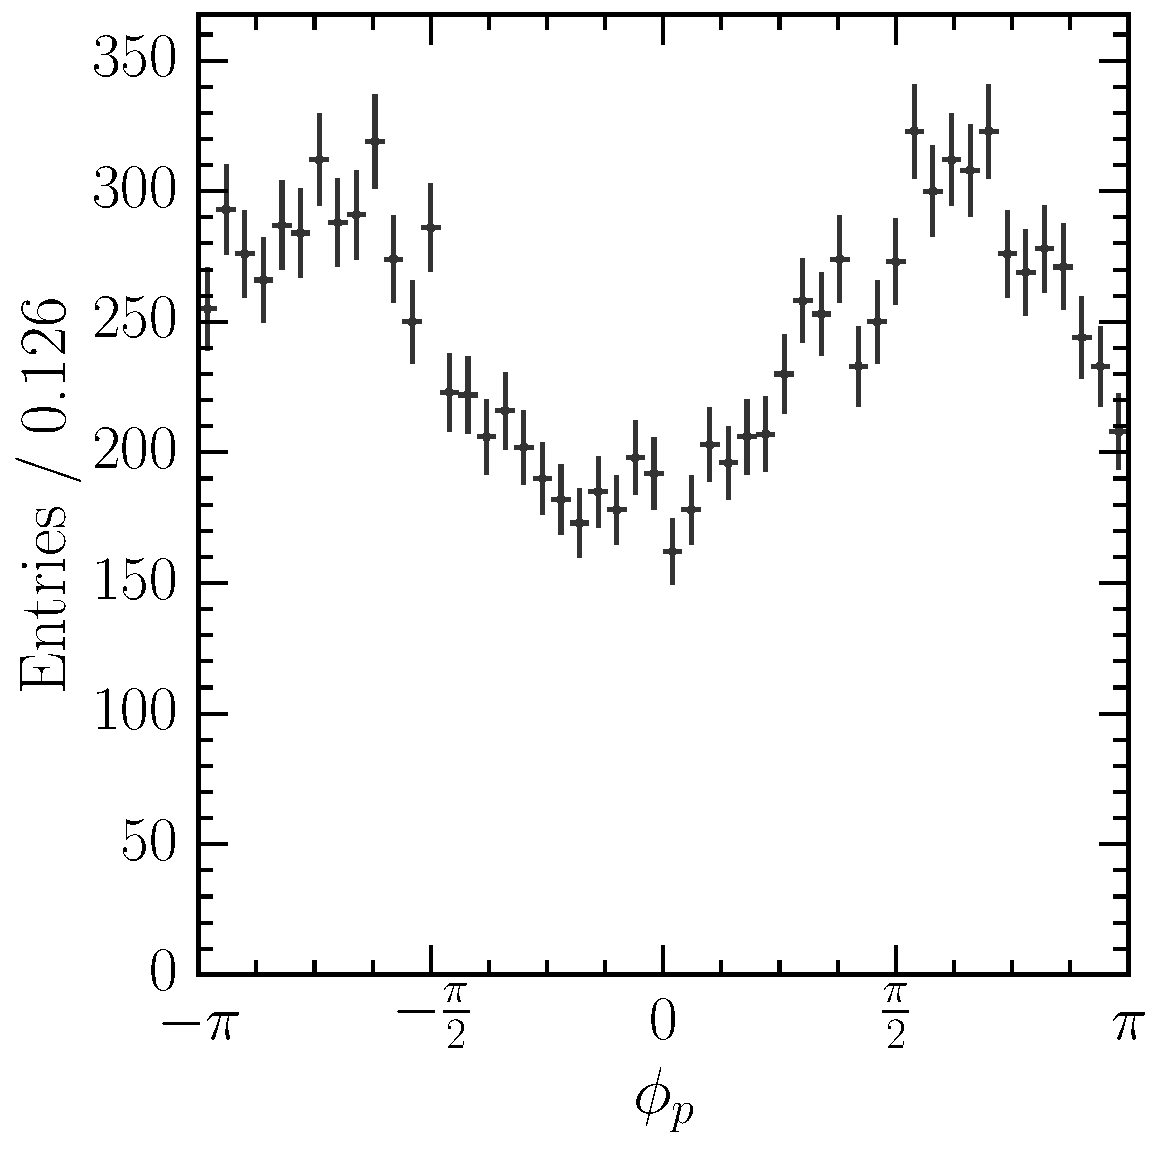
\includegraphics[width=\textwidth]{cpv/phase_space/LcTopKK_2012_MagDown_Lc_phsp_p_phi_after_selection}
    \label{fig:cpv:phsp:effs:pKK:Lc_phsp_p_phi:after}
  \end{subfigure}
  \begin{subfigure}{0.25\textwidth}
    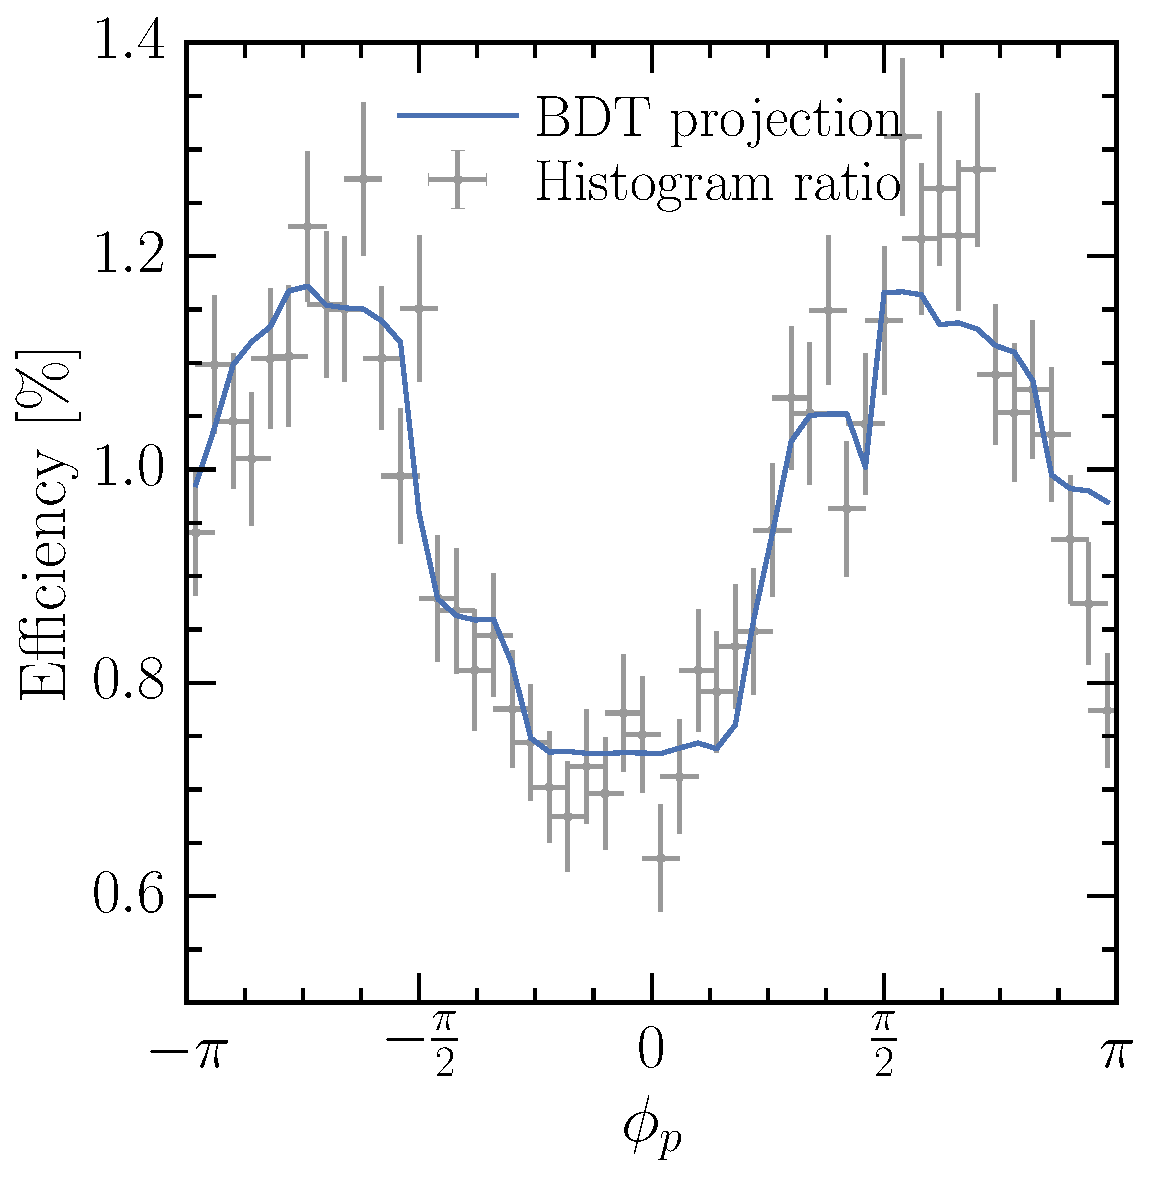
\includegraphics[width=\textwidth]{cpv/phase_space/LcTopKK_2012_MagDown_Lc_phsp_p_phi_efficiency}
    \label{fig:cpv:phsp:effs:pKK:Lc_phsp_p_phi:eff}
  \end{subfigure}

  \begin{subfigure}{0.25\textwidth}
    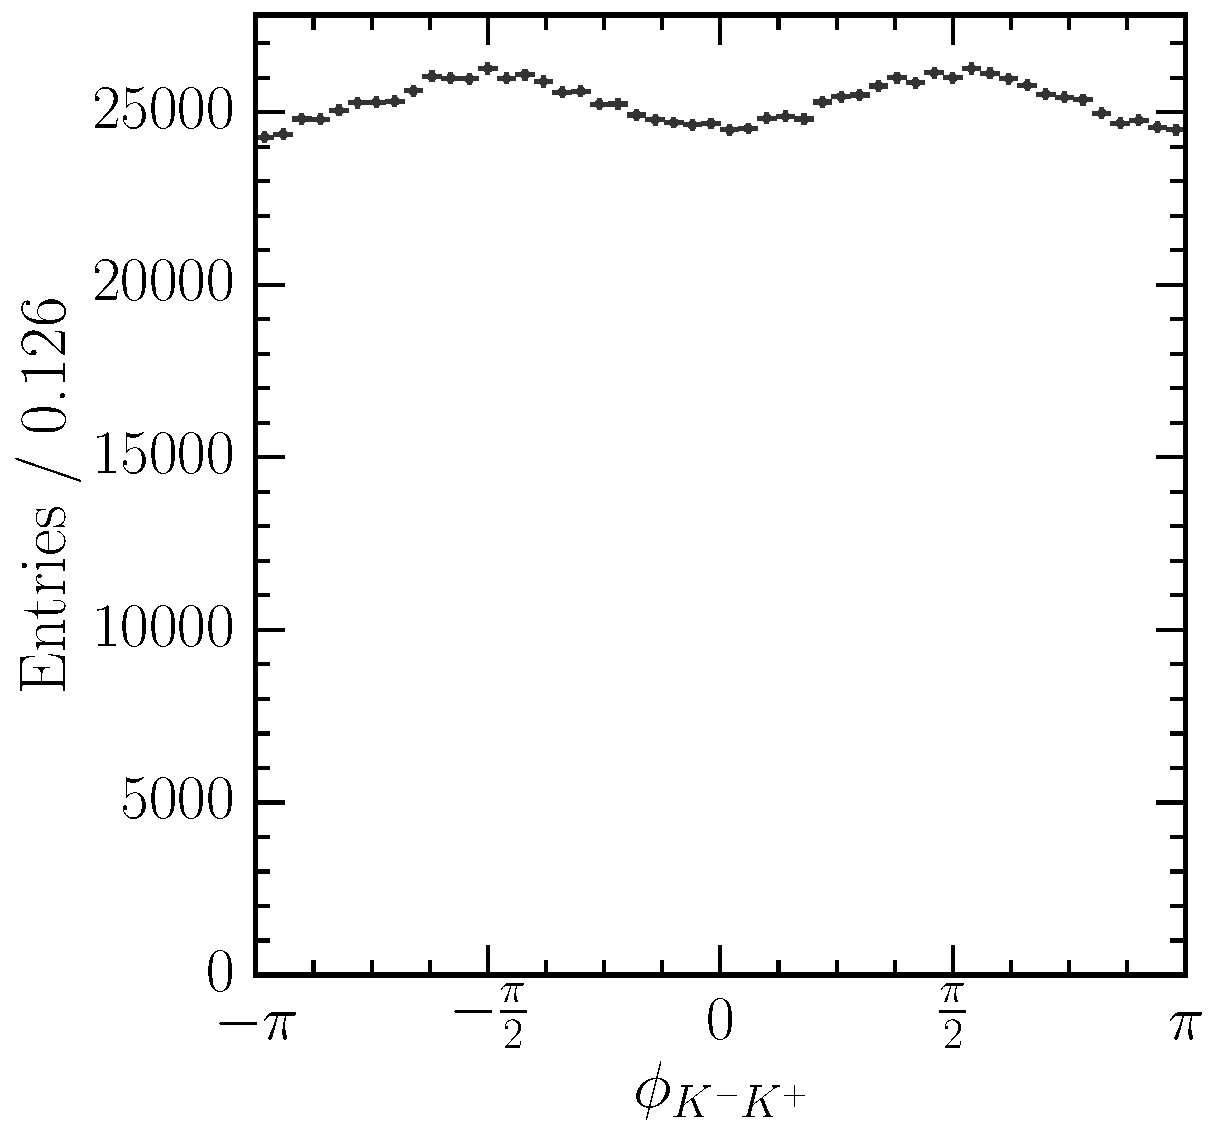
\includegraphics[width=\textwidth]{cpv/phase_space/LcTopKK_2012_MagDown_Lc_phsp_h1_h2_phi_before_selection}
    \label{fig:cpv:phsp:effs:pKK:Lc_phsp_h1_h2_phi:before}
  \end{subfigure}
  \begin{subfigure}{0.25\textwidth}
    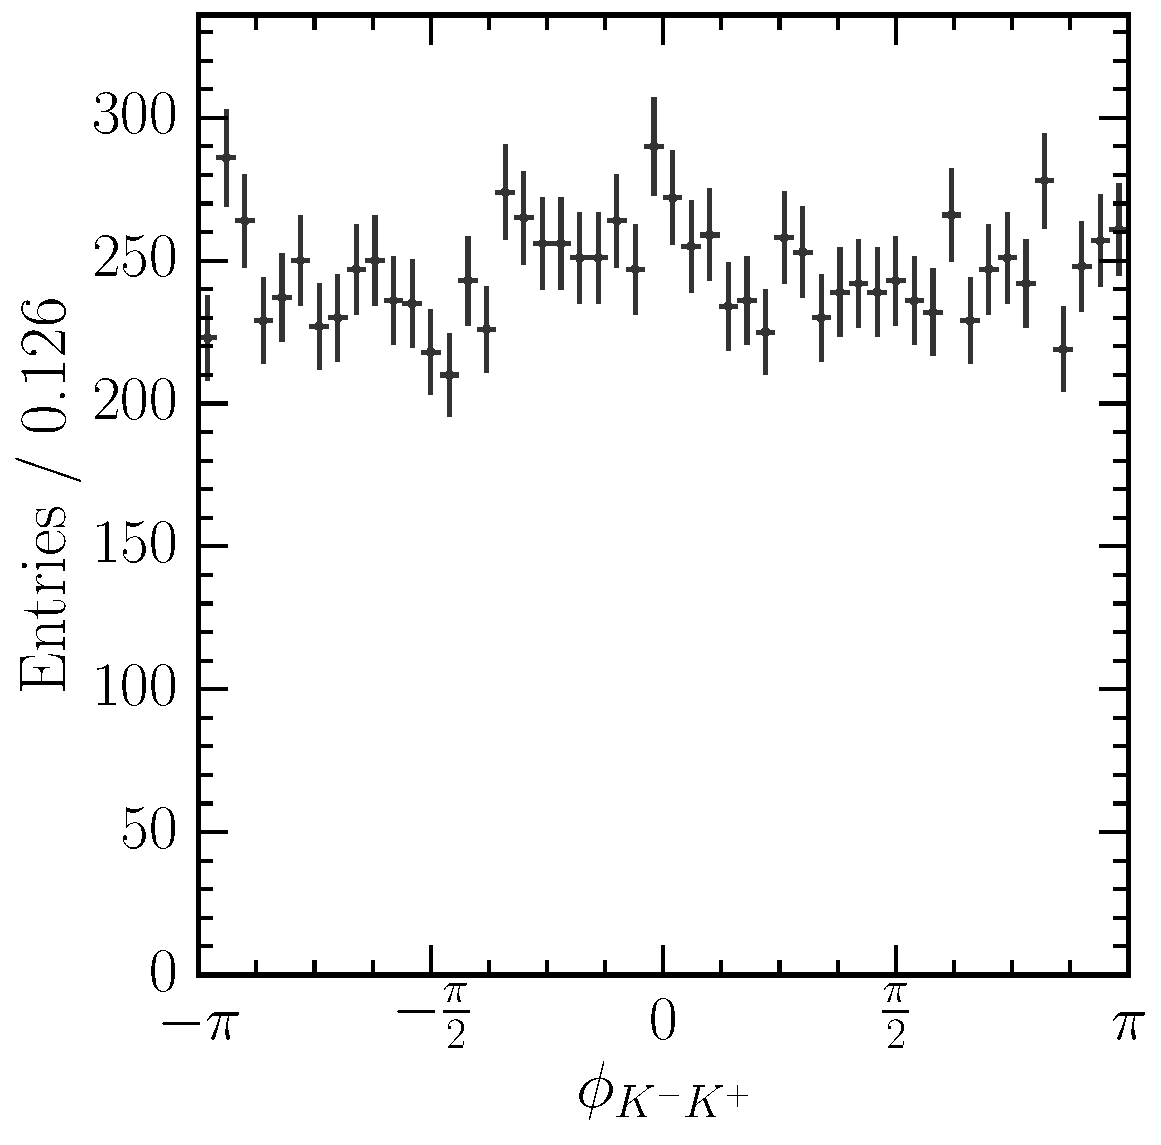
\includegraphics[width=\textwidth]{cpv/phase_space/LcTopKK_2012_MagDown_Lc_phsp_h1_h2_phi_after_selection}
    \label{fig:cpv:phsp:effs:pKK:Lc_phsp_h1_h2_phi:after}
  \end{subfigure}
  \begin{subfigure}{0.25\textwidth}
    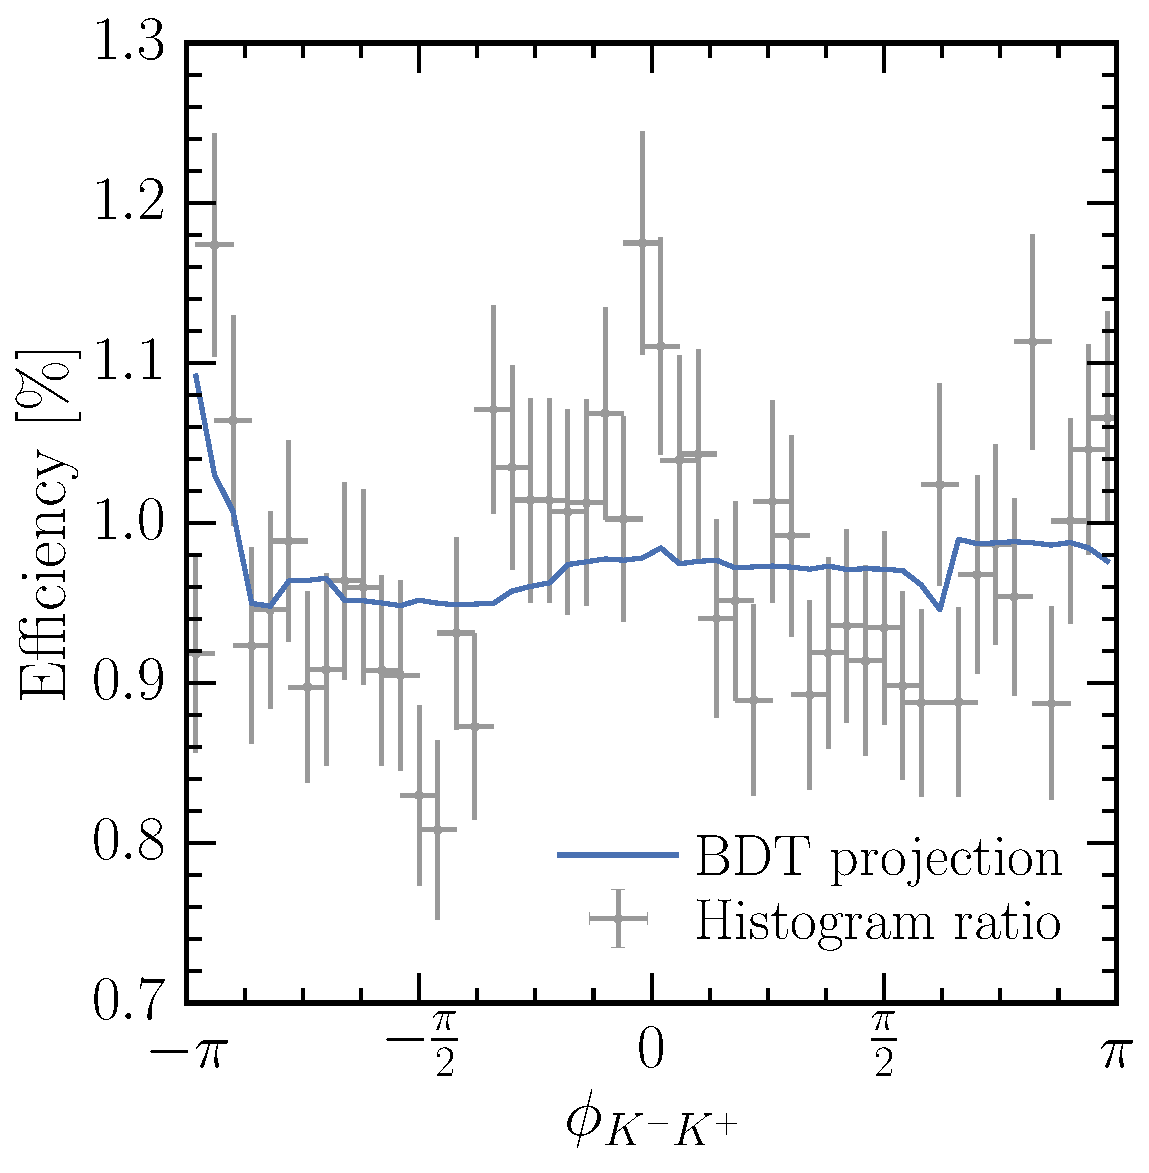
\includegraphics[width=\textwidth]{cpv/phase_space/LcTopKK_2012_MagDown_Lc_phsp_h1_h2_phi_efficiency}
    \label{fig:cpv:phsp:effs:pKK:Lc_phsp_h1_h2_phi:eff}
  \end{subfigure}

  \caption{%
    One dimensional projections of the \LcTopKK\ phase space in the 
    generator-level \ac{MC} (left column) and in the reconstructed and selected 
    \ac{MC} (centre column), for the 2012 magnet down simulation.
    The right column shows a one-dimensional projection efficiency curve learnt 
    by a \ac{BDT} trained to weight the generator-level \ac{MC} to look like 
    the reconstructed and selected \ac{MC}.
    For comparison, a ratio of the histograms is also shown with the curve.
  }
  \label{fig:cpv:phsp:effs:pKK}
\end{figure}

\begin{figure}
  \centering

  \begin{subfigure}{0.25\textwidth}
    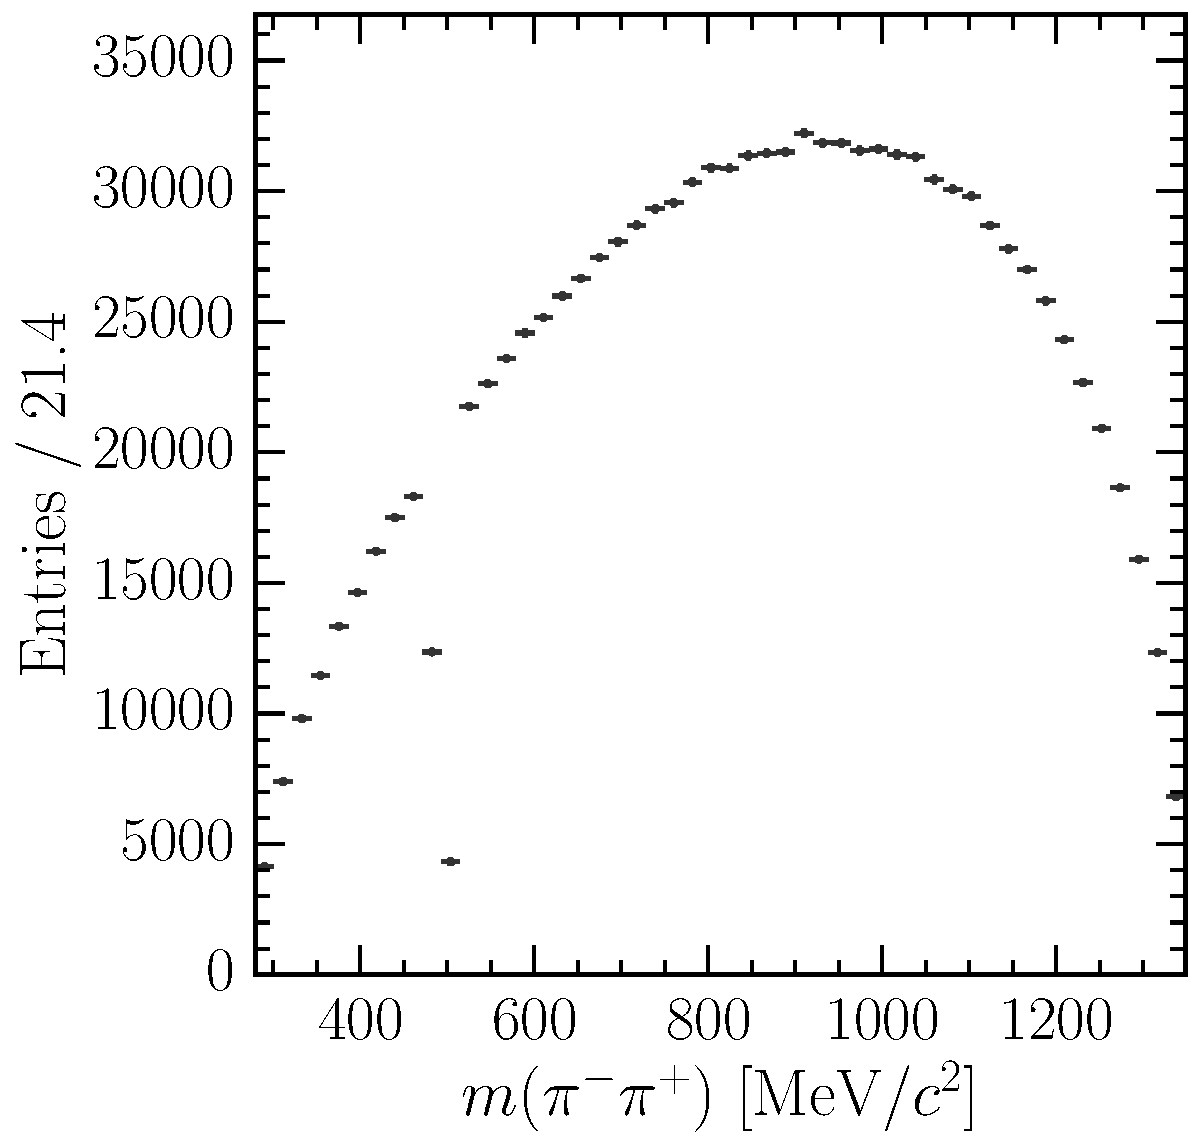
\includegraphics[width=\textwidth]{cpv/phase_space/LcToppipi_2012_MagDown_Lc_h1_h2_M_before_selection}
    \label{fig:cpv:phsp:effs:ppipi:Lc_h1_h2_M:before}
  \end{subfigure}
  \begin{subfigure}{0.25\textwidth}
    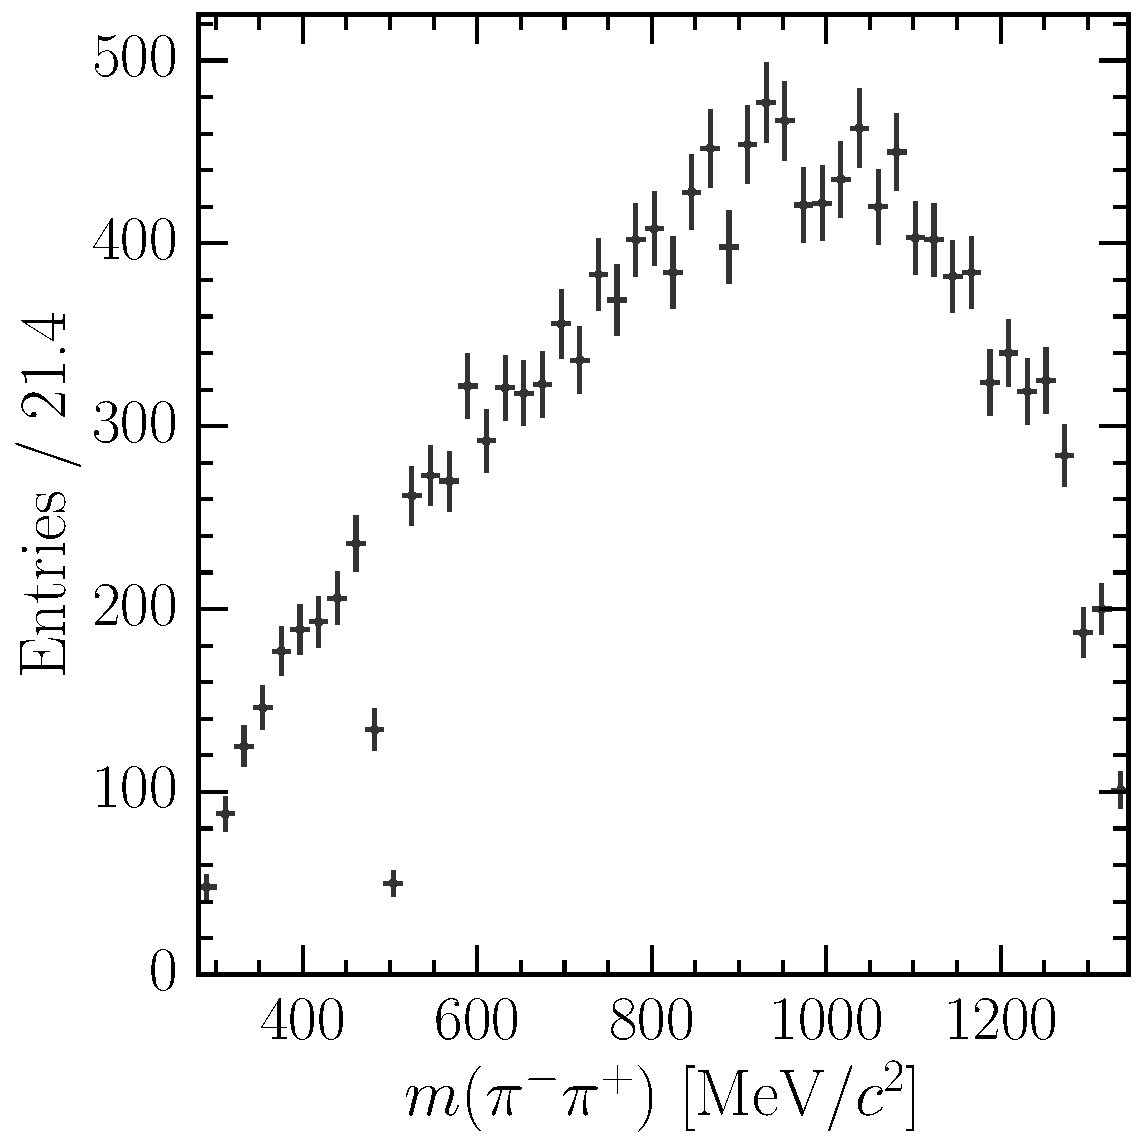
\includegraphics[width=\textwidth]{cpv/phase_space/LcToppipi_2012_MagDown_Lc_h1_h2_M_after_selection}
    \label{fig:cpv:phsp:effs:ppipi:Lc_h1_h2_M:after}
  \end{subfigure}
  \begin{subfigure}{0.25\textwidth}
    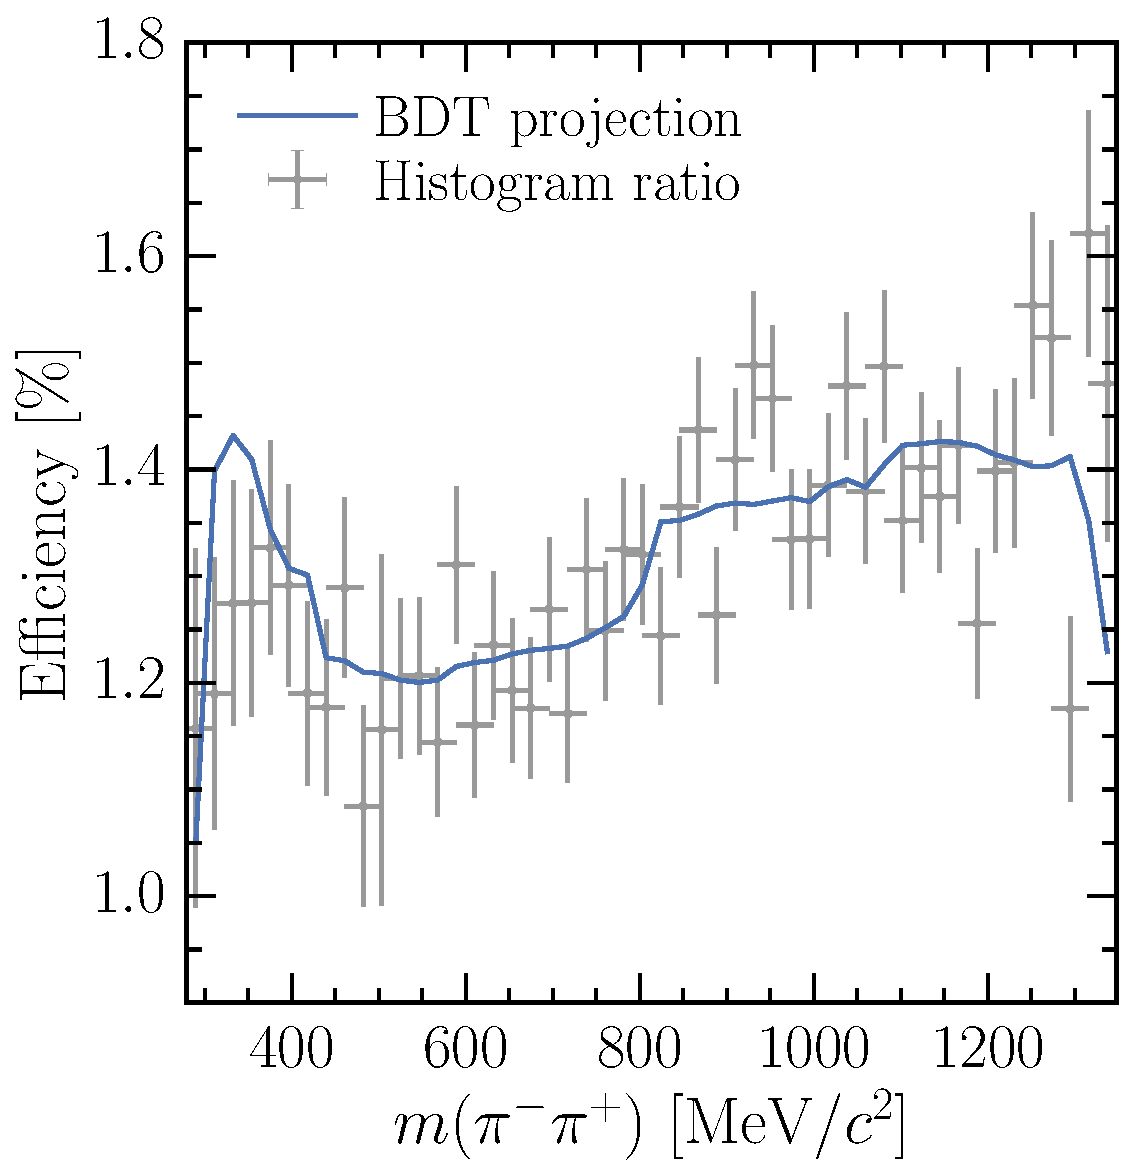
\includegraphics[width=\textwidth]{cpv/phase_space/LcToppipi_2012_MagDown_Lc_h1_h2_M_efficiency}
    \label{fig:cpv:phsp:effs:ppipi:Lc_h1_h2_M:eff}
  \end{subfigure}

  \begin{subfigure}{0.25\textwidth}
    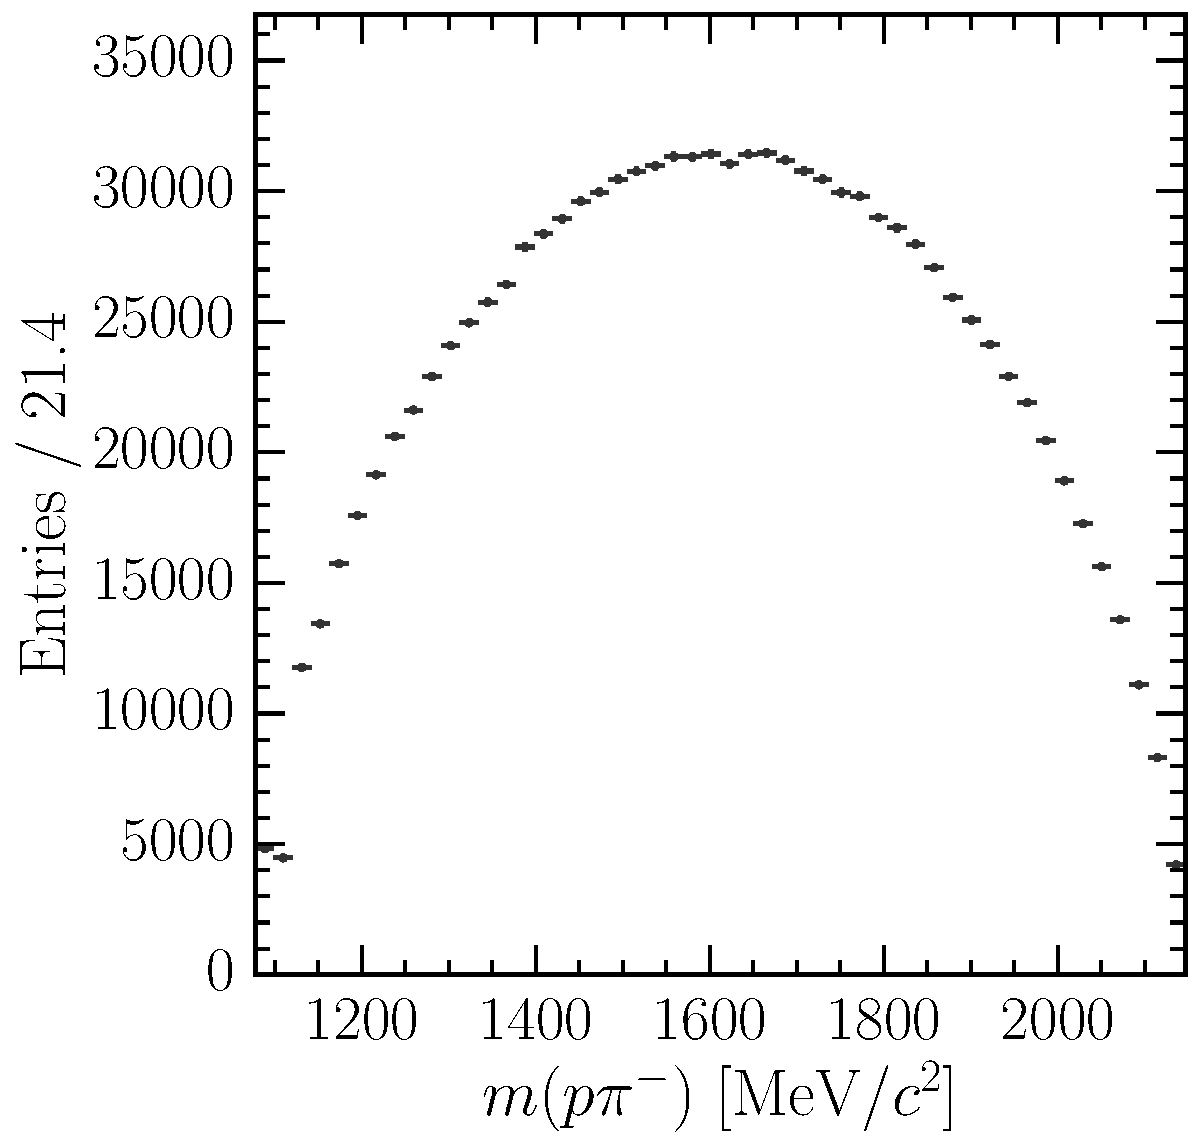
\includegraphics[width=\textwidth]{cpv/phase_space/LcToppipi_2012_MagDown_Lc_p_h1_M_before_selection}
    \label{fig:cpv:phsp:effs:ppipi:Lc_p_h1_M:before}
  \end{subfigure}
  \begin{subfigure}{0.25\textwidth}
    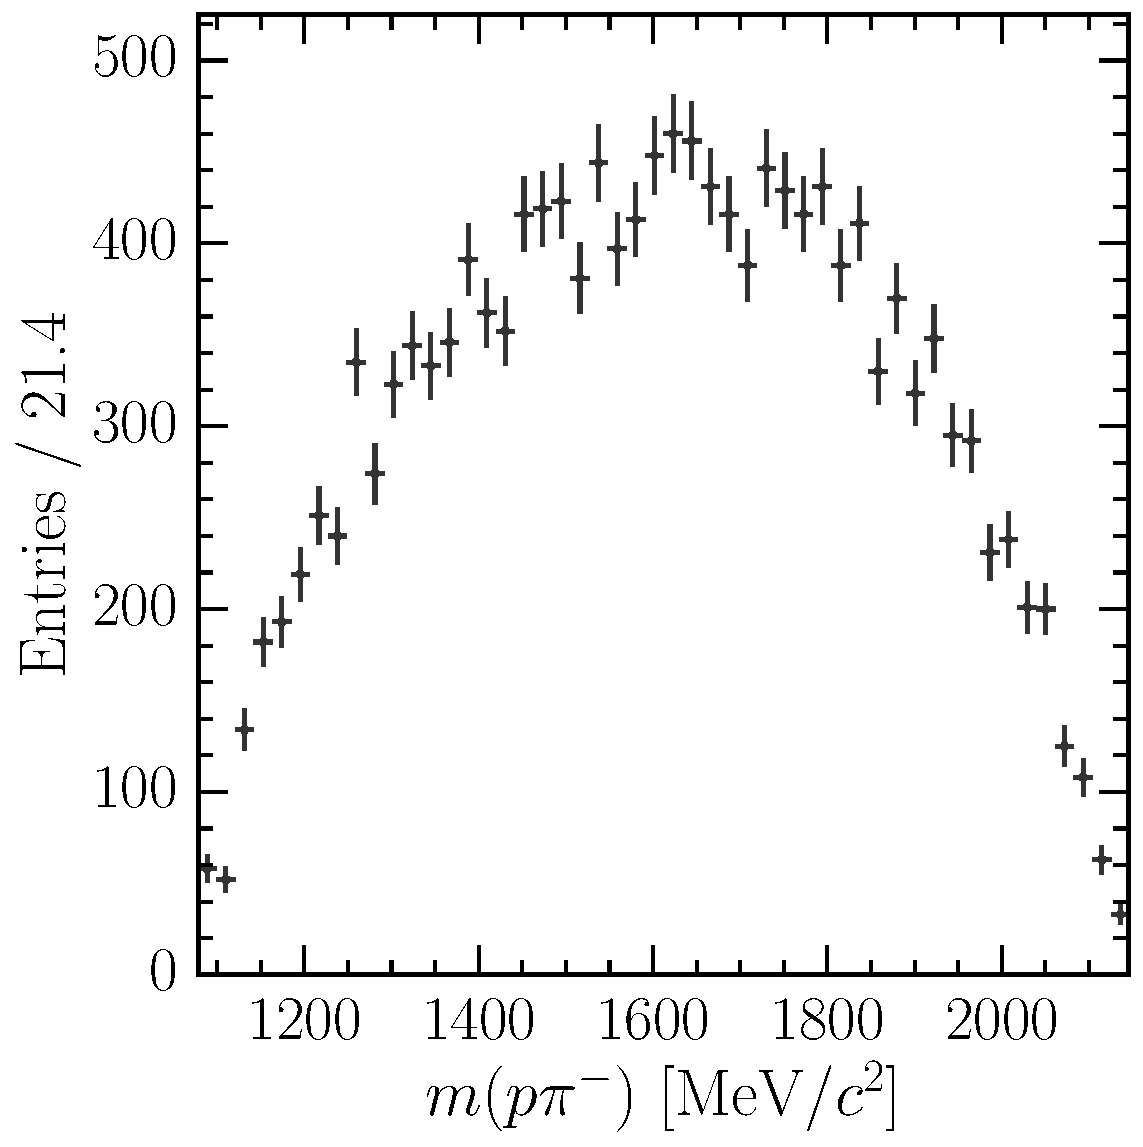
\includegraphics[width=\textwidth]{cpv/phase_space/LcToppipi_2012_MagDown_Lc_p_h1_M_after_selection}
    \label{fig:cpv:phsp:effs:ppipi:Lc_p_h1_M:after}
  \end{subfigure}
  \begin{subfigure}{0.25\textwidth}
    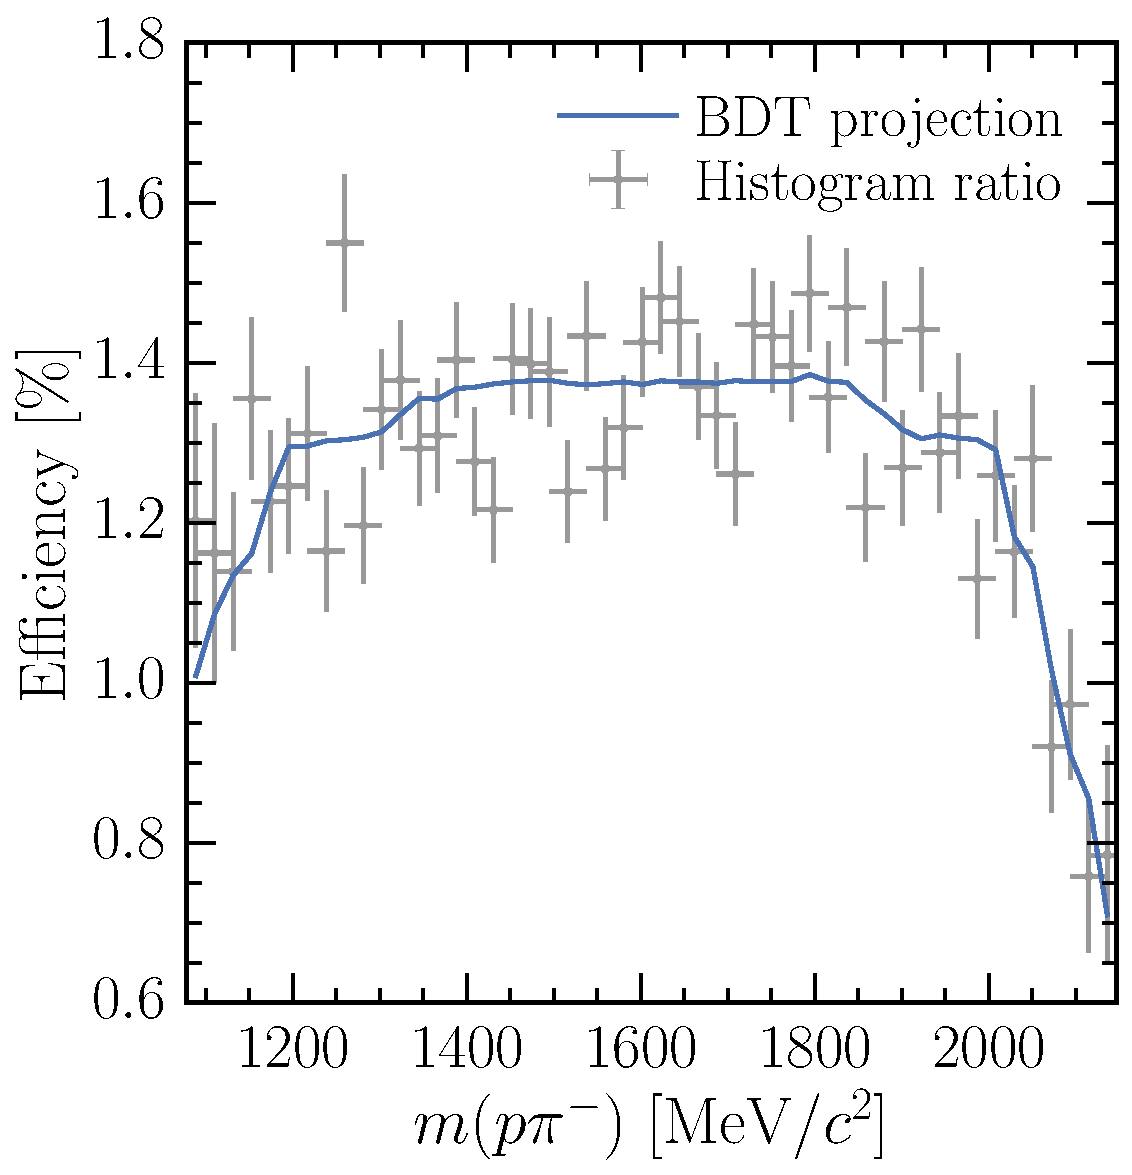
\includegraphics[width=\textwidth]{cpv/phase_space/LcToppipi_2012_MagDown_Lc_p_h1_M_efficiency}
    \label{fig:cpv:phsp:effs:ppipi:Lc_p_h1_M:eff}
  \end{subfigure}

  \begin{subfigure}{0.25\textwidth}
    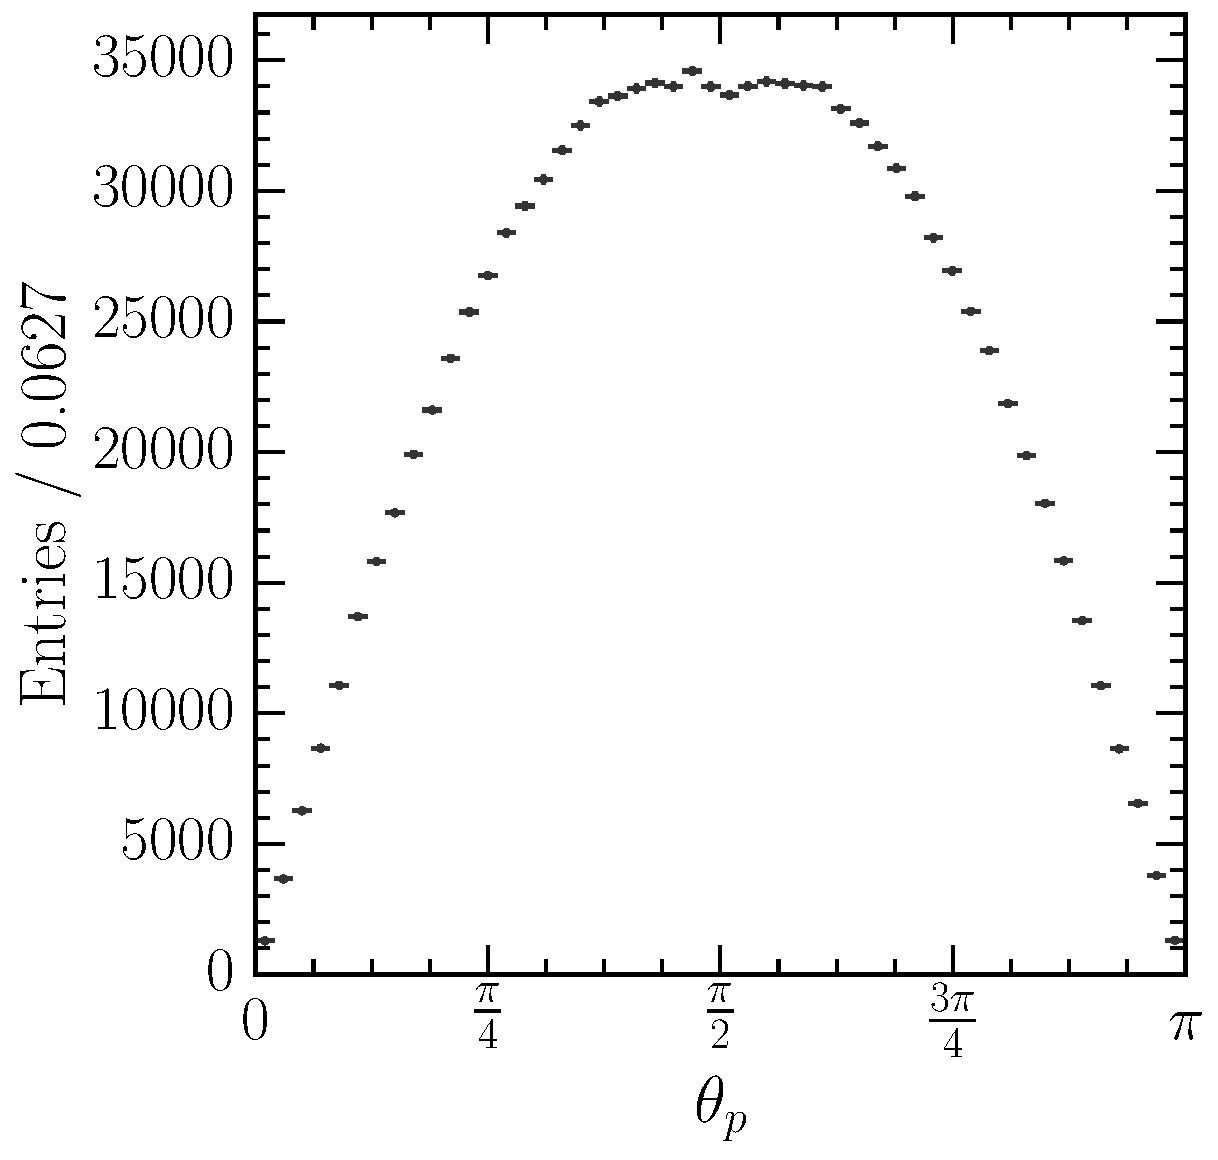
\includegraphics[width=\textwidth]{cpv/phase_space/LcToppipi_2012_MagDown_Lc_phsp_p_theta_before_selection}
    \label{fig:cpv:phsp:effs:ppipi:Lc_phsp_p_theta:before}
  \end{subfigure}
  \begin{subfigure}{0.25\textwidth}
    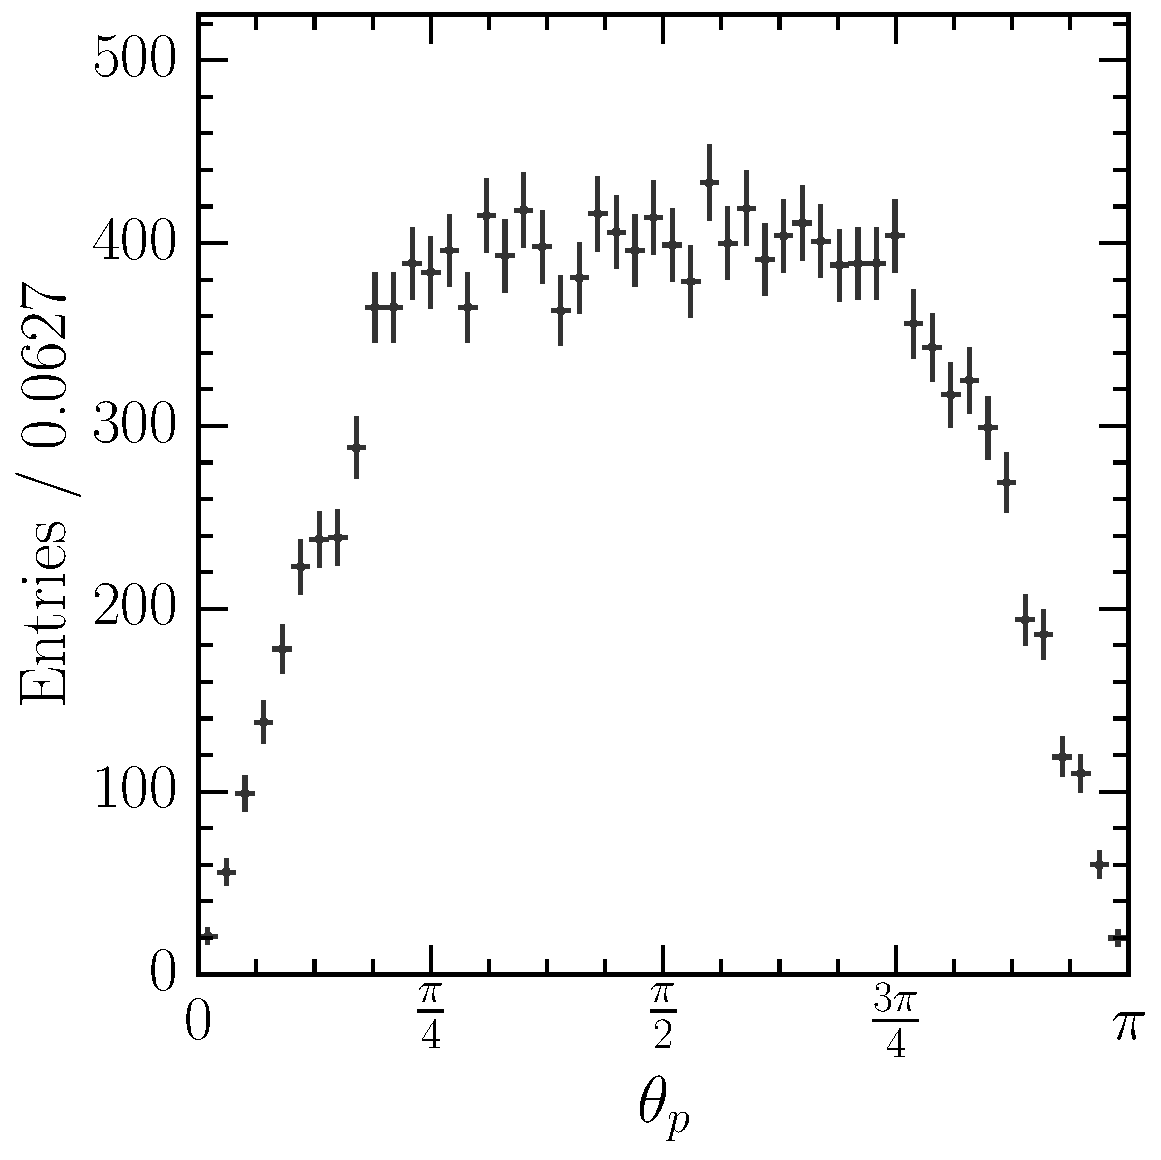
\includegraphics[width=\textwidth]{cpv/phase_space/LcToppipi_2012_MagDown_Lc_phsp_p_theta_after_selection}
    \label{fig:cpv:phsp:effs:ppipi:Lc_phsp_p_theta:after}
  \end{subfigure}
  \begin{subfigure}{0.25\textwidth}
    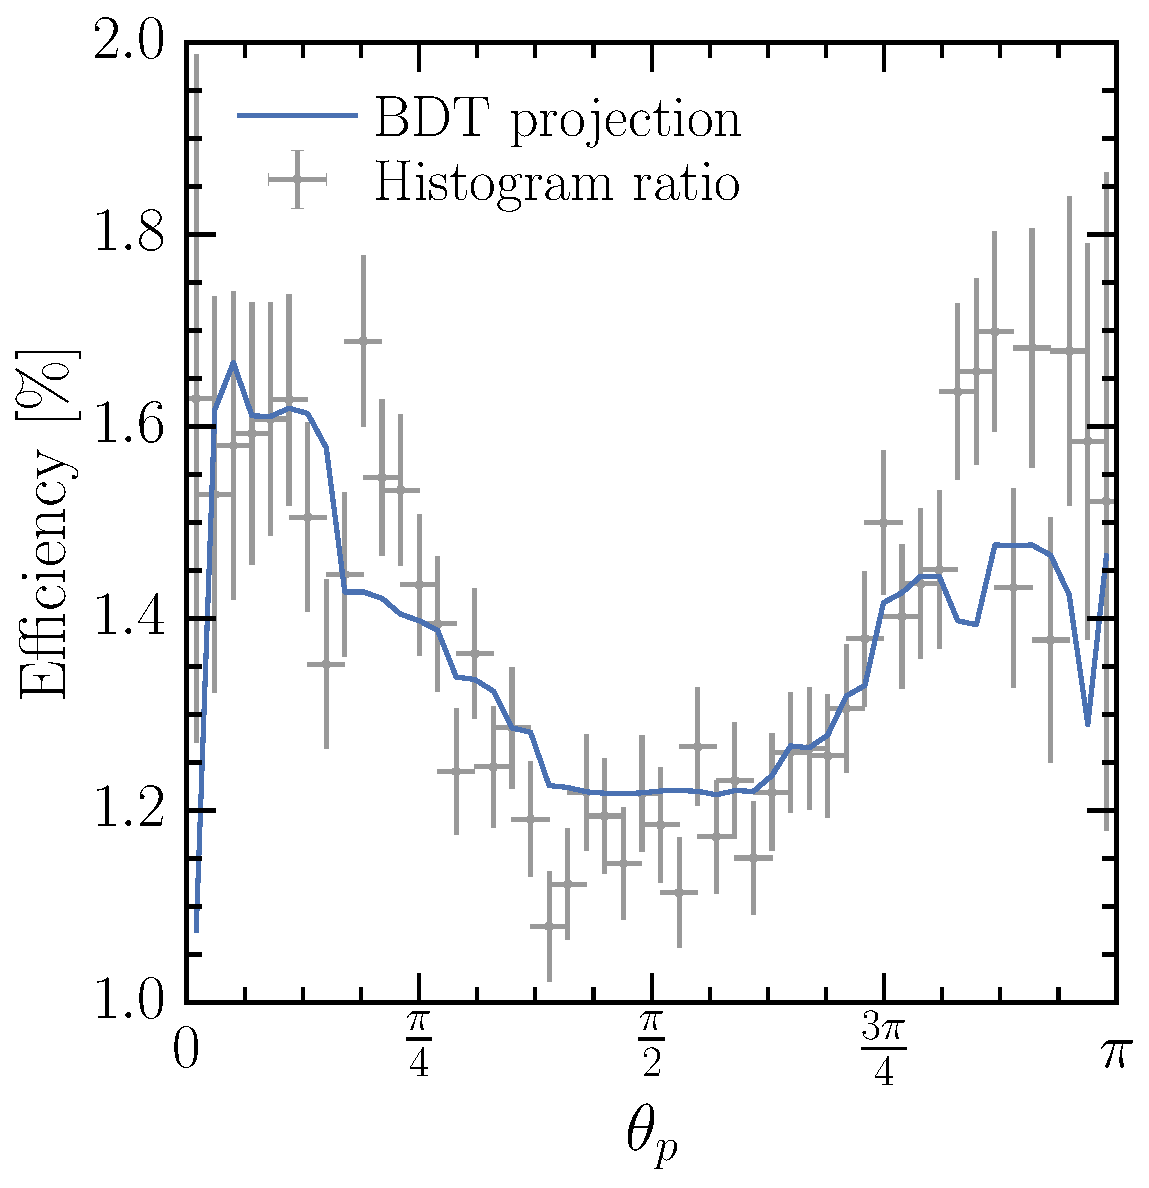
\includegraphics[width=\textwidth]{cpv/phase_space/LcToppipi_2012_MagDown_Lc_phsp_p_theta_efficiency}
    \label{fig:cpv:phsp:effs:ppipi:Lc_phsp_p_theta:eff}
  \end{subfigure}

  \begin{subfigure}{0.25\textwidth}
    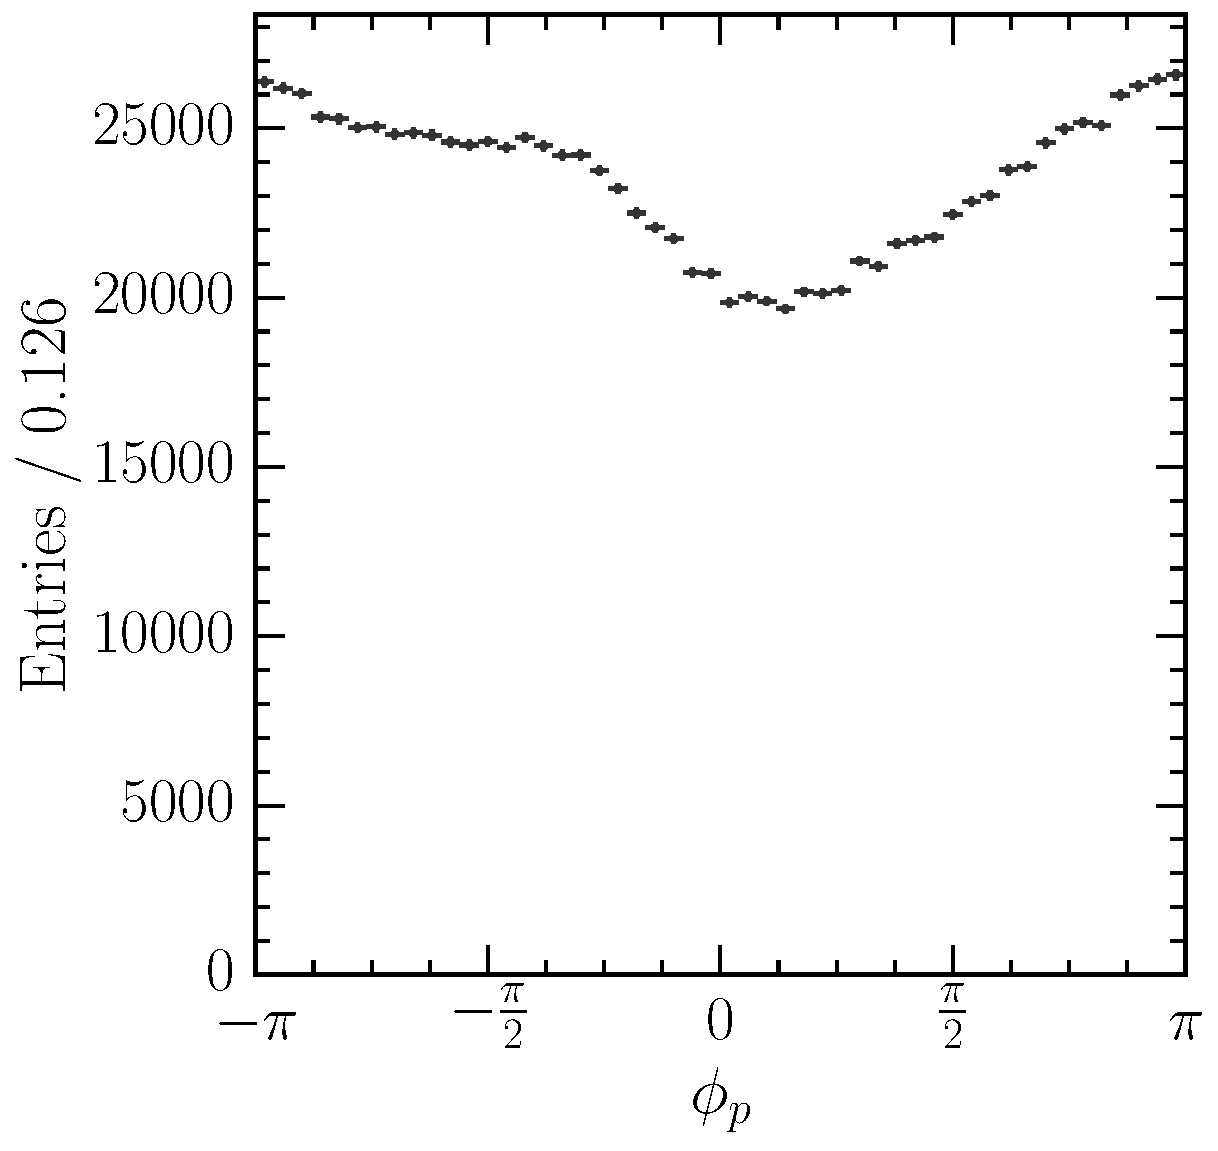
\includegraphics[width=\textwidth]{cpv/phase_space/LcToppipi_2012_MagDown_Lc_phsp_p_phi_before_selection}
    \label{fig:cpv:phsp:effs:ppipi:Lc_phsp_p_phi:before}
  \end{subfigure}
  \begin{subfigure}{0.25\textwidth}
    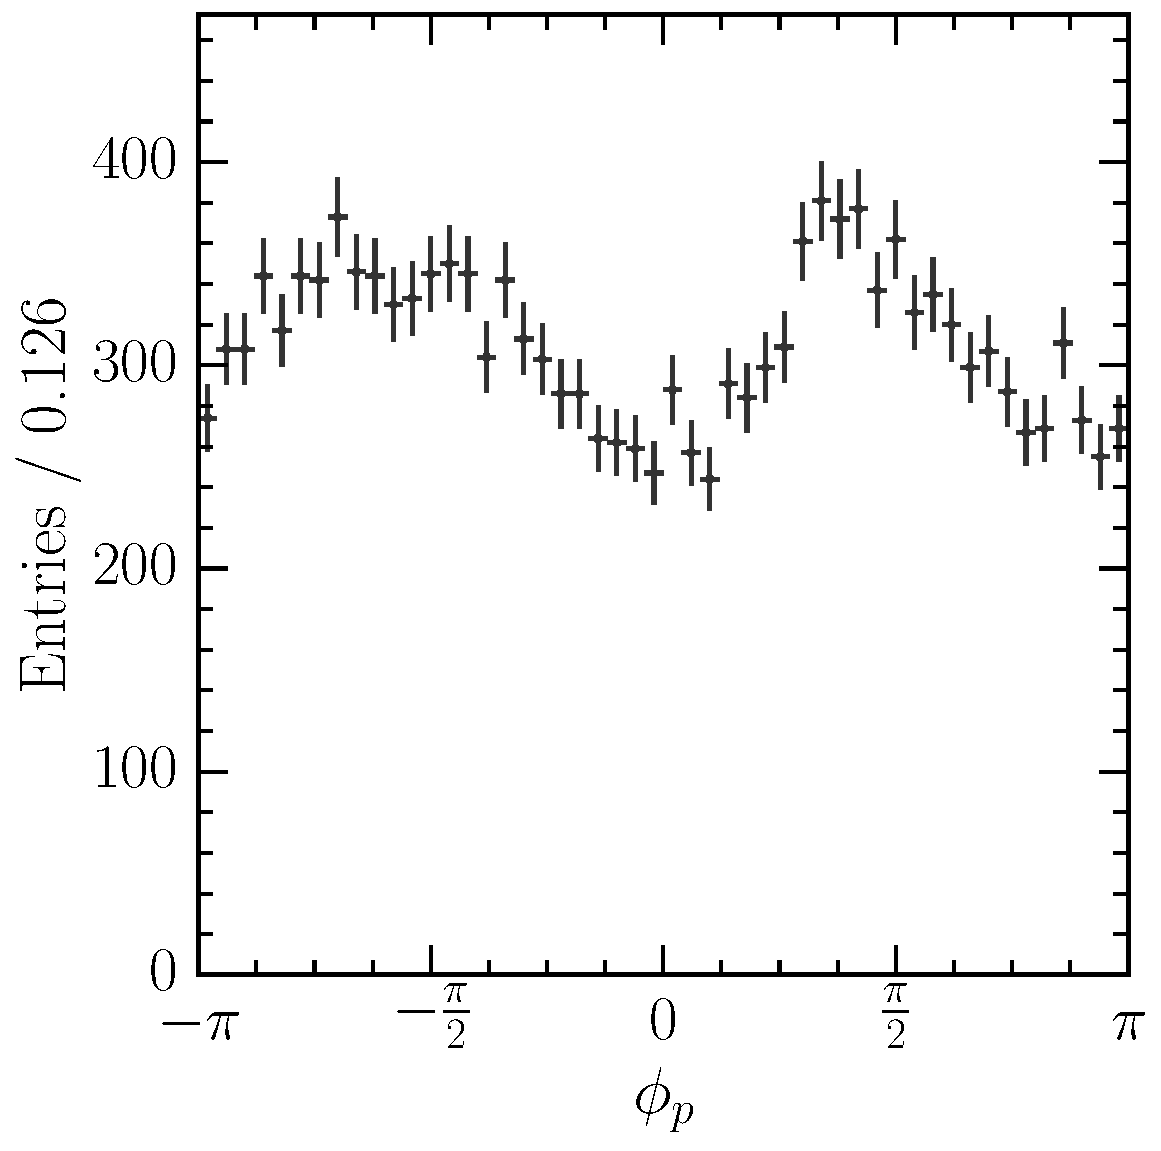
\includegraphics[width=\textwidth]{cpv/phase_space/LcToppipi_2012_MagDown_Lc_phsp_p_phi_after_selection}
    \label{fig:cpv:phsp:effs:ppipi:Lc_phsp_p_phi:after}
  \end{subfigure}
  \begin{subfigure}{0.25\textwidth}
    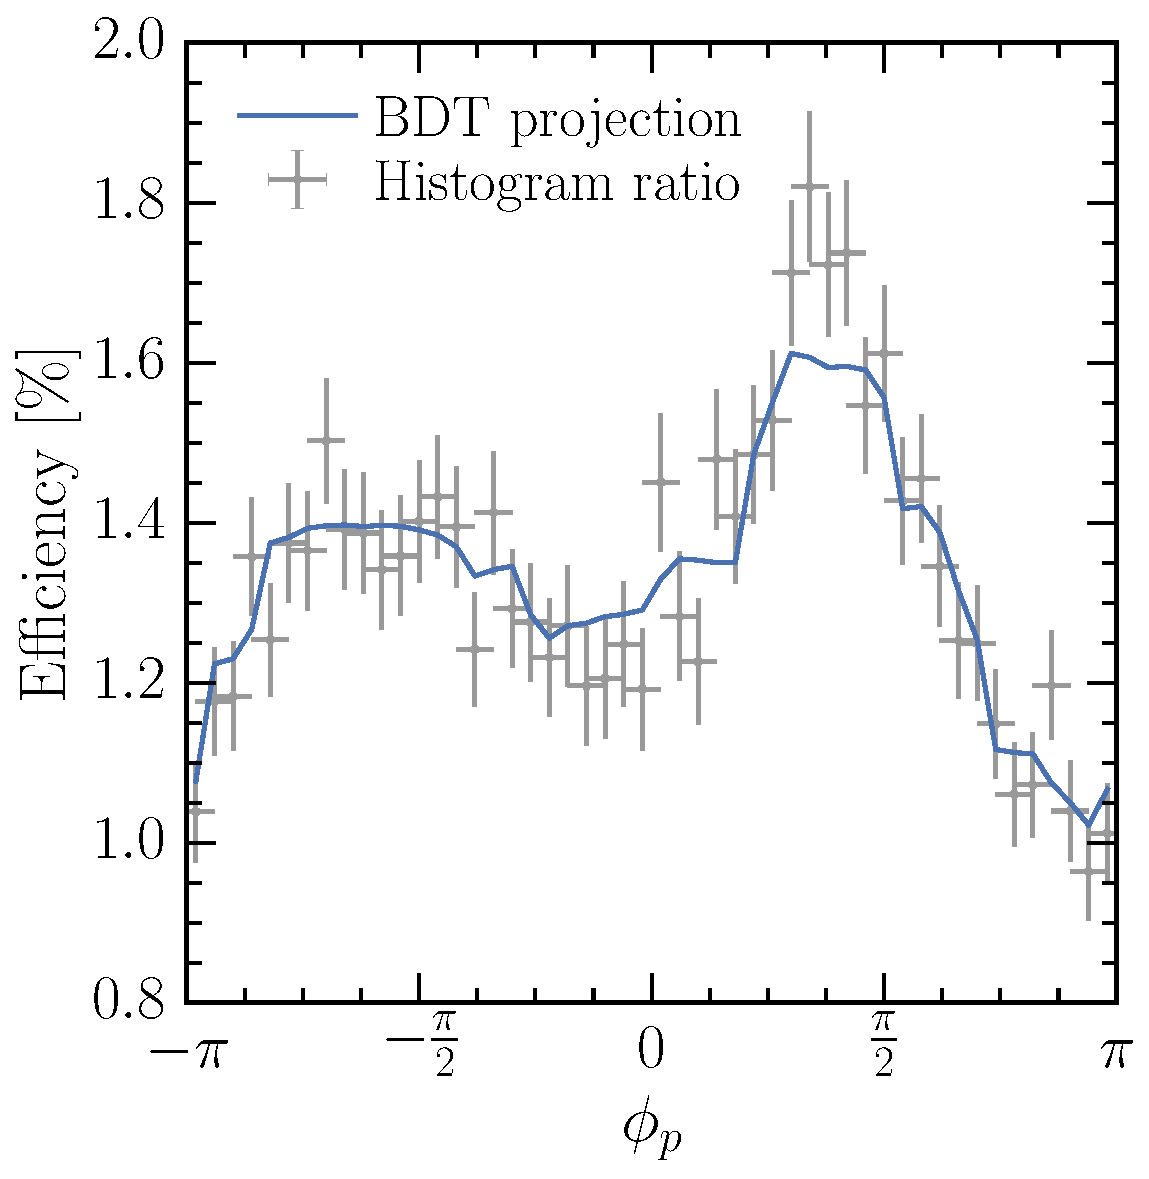
\includegraphics[width=\textwidth]{cpv/phase_space/LcToppipi_2012_MagDown_Lc_phsp_p_phi_efficiency}
    \label{fig:cpv:phsp:effs:ppipi:Lc_phsp_p_phi:eff}
  \end{subfigure}

  \begin{subfigure}{0.25\textwidth}
    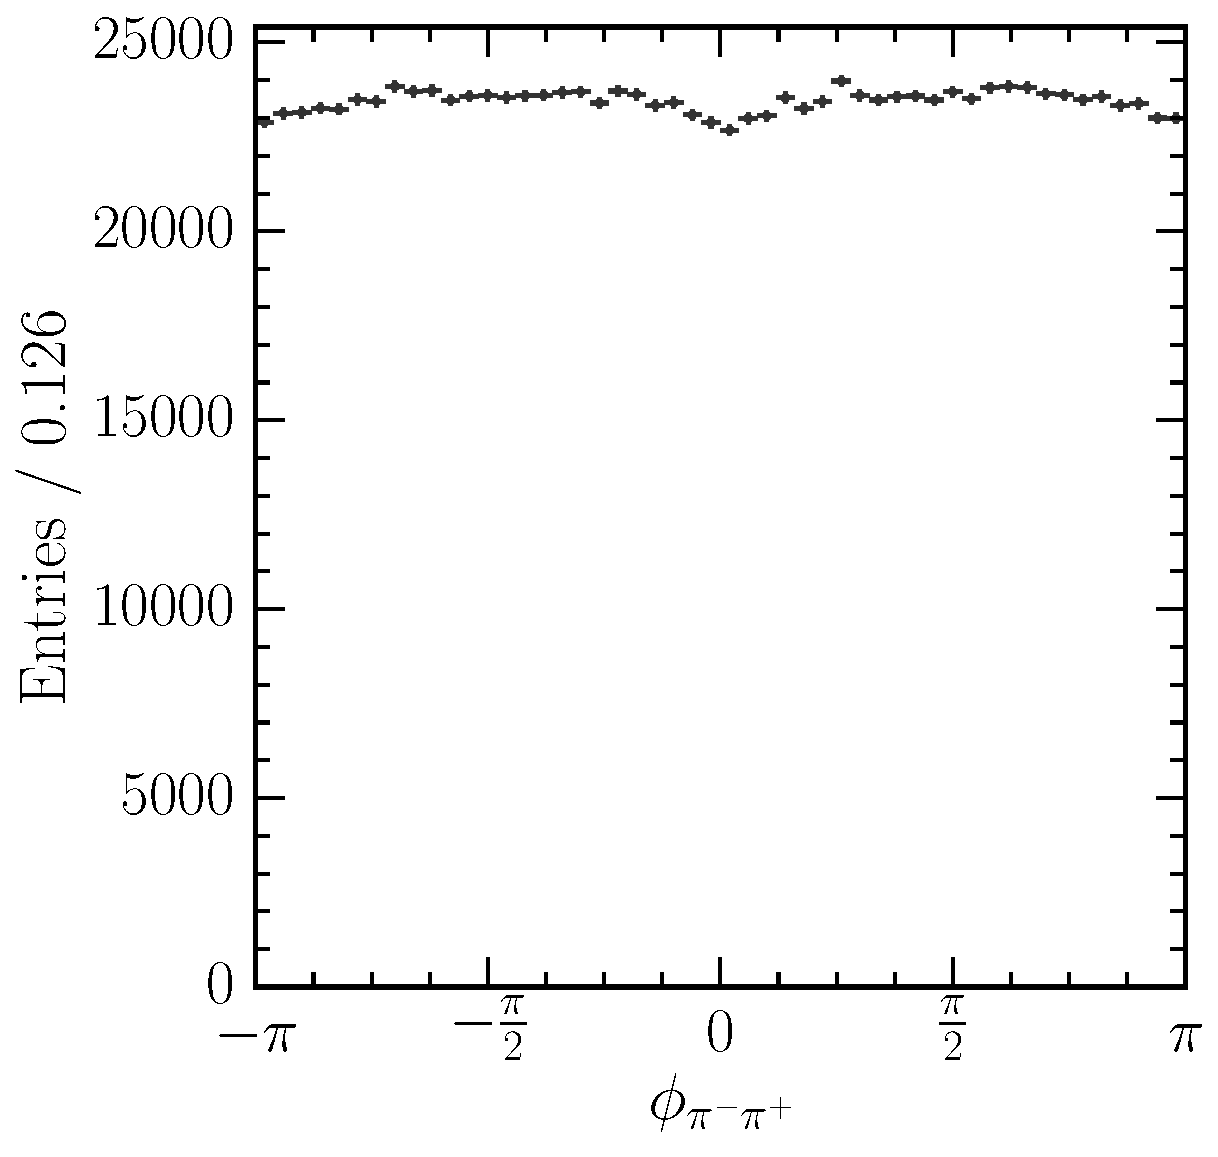
\includegraphics[width=\textwidth]{cpv/phase_space/LcToppipi_2012_MagDown_Lc_phsp_h1_h2_phi_before_selection}
    \label{fig:cpv:phsp:effs:ppipi:Lc_phsp_h1_h2_phi:before}
  \end{subfigure}
  \begin{subfigure}{0.25\textwidth}
    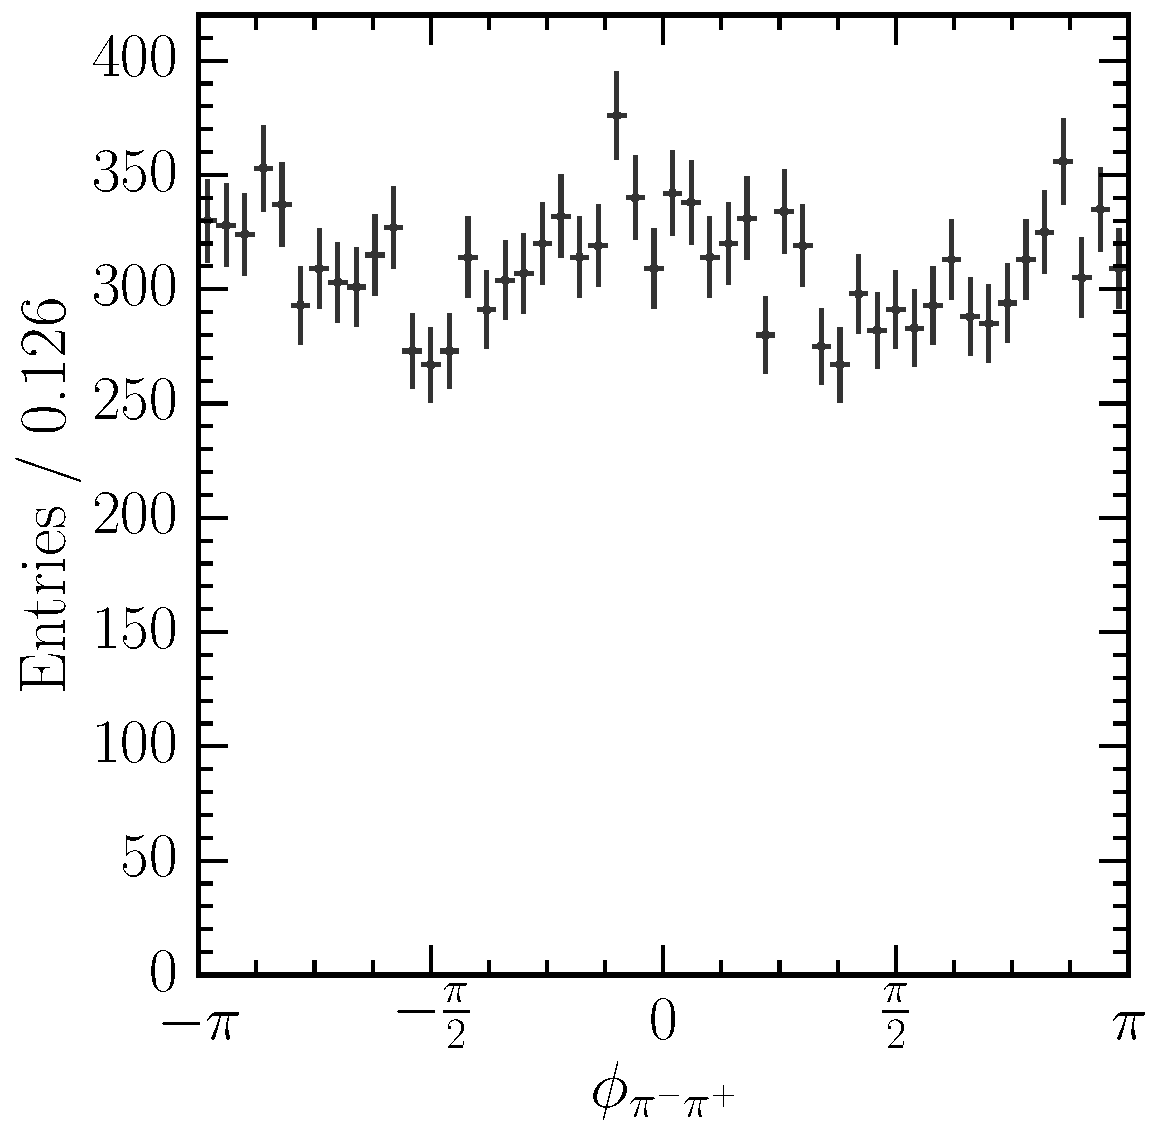
\includegraphics[width=\textwidth]{cpv/phase_space/LcToppipi_2012_MagDown_Lc_phsp_h1_h2_phi_after_selection}
    \label{fig:cpv:phsp:effs:ppipi:Lc_phsp_h1_h2_phi:after}
  \end{subfigure}
  \begin{subfigure}{0.25\textwidth}
    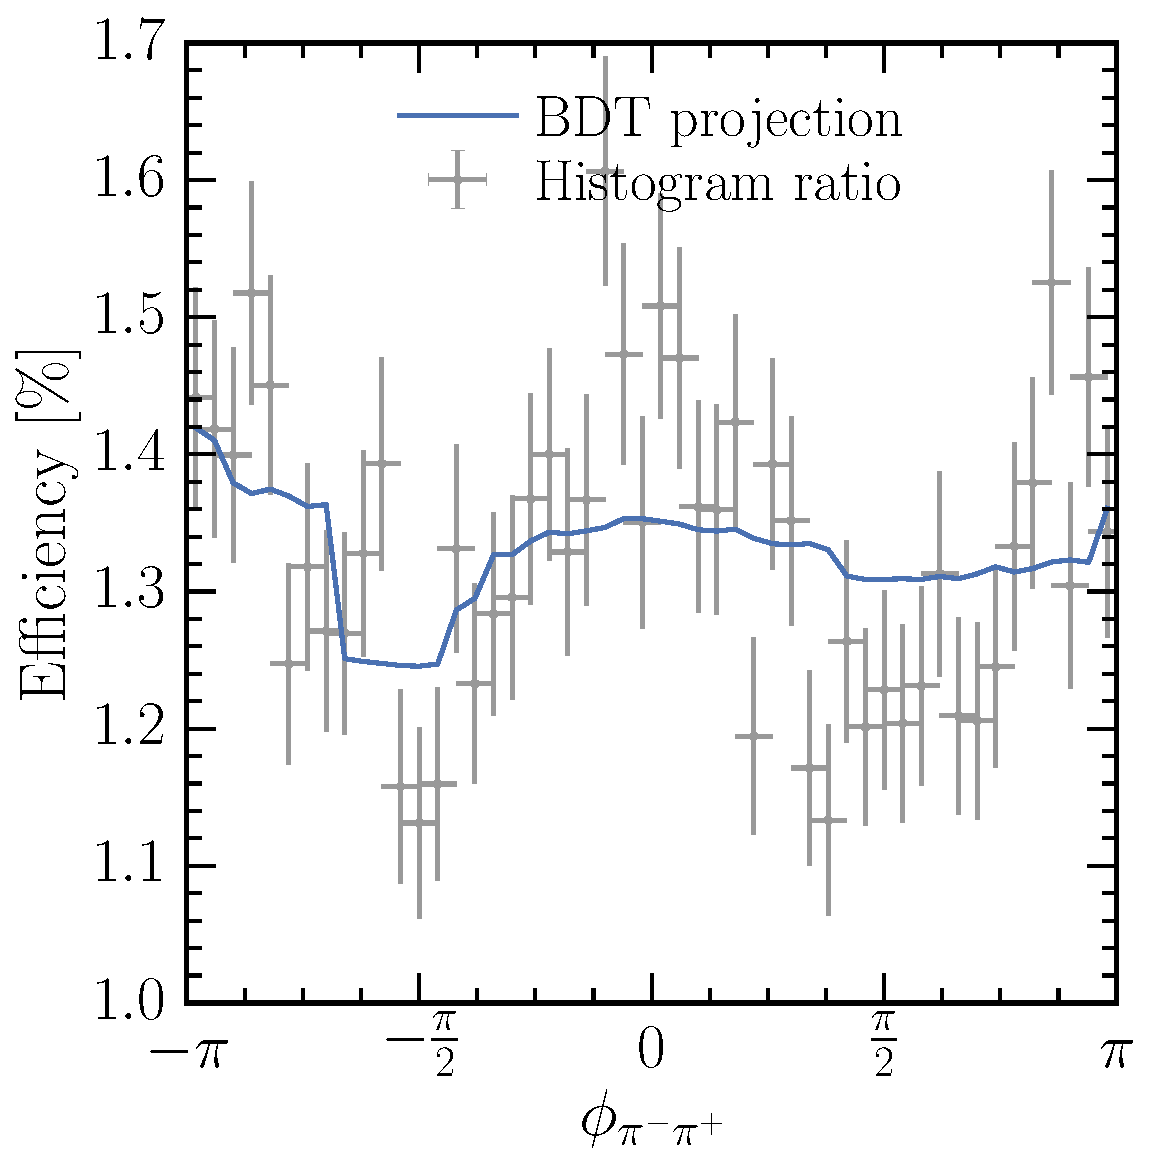
\includegraphics[width=\textwidth]{cpv/phase_space/LcToppipi_2012_MagDown_Lc_phsp_h1_h2_phi_efficiency}
    \label{fig:cpv:phsp:effs:ppipi:Lc_phsp_h1_h2_phi:eff}
  \end{subfigure}

  \caption{%
    One dimensional projections of the \LcToppipi\ phase space in the 
    generator-level \ac{MC} (left column) and in the reconstructed and selected 
    \ac{MC} (centre column), for the 2012 magnet down simulation.
    The right column shows a one-dimensional projection efficiency curve learnt 
    by a \ac{BDT} trained to weight the generator-level \ac{MC} to look like 
    the reconstructed and selected \ac{MC}.
    For comparison, a ratio of the histograms is also shown with the curve.
  }
  \label{fig:cpv:phsp:effs:ppipi}
\end{figure}
